% !TEX program = xelatex
\documentclass[UTF8,fontset=fandol,a4paper,11pt]{ctexart}
\usepackage[margin=21mm,top=23mm,bottom=22mm,headheight=16pt]{geometry}
\usepackage{amsmath,amssymb,mathtools,bm}
\usepackage{tikz}
\usetikzlibrary{arrows.meta,calc,angles,quotes,patterns}
\usepackage{xcolor,booktabs,array,longtable,enumitem,fancyhdr,needspace}
\usepackage[unicode,hidelinks]{hyperref}
\definecolor{ink}{HTML}{24343C}
\definecolor{accent}{HTML}{166A70}
\definecolor{muted}{HTML}{65747A}
\definecolor{rulegray}{HTML}{D4DDE0}
\definecolor{warm}{HTML}{966037}
\color{ink}
\setlength{\parindent}{2em}
\setlength{\parskip}{4pt}
\linespread{1.12}
\AtBeginDocument{\setlength{\abovedisplayskip}{6pt plus 2pt minus 1pt}
\setlength{\belowdisplayskip}{6pt plus 2pt minus 1pt}
\setlength{\abovedisplayshortskip}{0pt plus 1pt}
\setlength{\belowdisplayshortskip}{4pt plus 1pt}}
\setlist[enumerate]{label=(\arabic*),leftmargin=2.3em,itemsep=3pt,topsep=4pt}
\setlist[itemize]{leftmargin=2em,itemsep=2pt,topsep=4pt}
\allowdisplaybreaks[1]
\setlength{\emergencystretch}{2em}
\setcounter{secnumdepth}{0}
\providecommand{\tightlist}{\setlength{\itemsep}{0pt}\setlength{\parskip}{0pt}}
\ctexset{section={format=\Large\bfseries\color{accent},beforeskip=10pt,afterskip=9pt},
subsection={format=\normalsize\bfseries\color{accent},beforeskip=10pt,afterskip=4pt},
subsubsection={format=\normalsize\bfseries,beforeskip=8pt,afterskip=3pt}}
\pagestyle{fancy}
\fancyhf{}
\fancyhead[L]{\small\color{muted}物理学难题集萃}
% 页眉仅保留书名；版本名称只在封面显示。
\fancyfoot[L]{\small\color{muted}\chapterlabel}
\fancyfoot[R]{\small\thepage}
\renewcommand{\headrulewidth}{0.4pt}
\renewcommand{\footrulewidth}{0pt}
\newcommand{\dd}{\mathop{}\!\mathrm{d}}
\newcommand{\vect}[1]{\bm{#1}}
\newcommand{\tagline}[1]{\noindent{\small\color{muted}#1}\par}
\newcommand{\result}[1]{\begin{equation*}\boxed{#1}\end{equation*}}
\newcommand{\figcaption}[1]{\par\vspace{2pt}{\small\color{muted}#1}\par}
\newcommand{\teach}[2]{\Needspace{4\baselineskip}\subsection*{讲解要点与追问}#1\par\smallskip\noindent\textbf{追问：}#2\par}
\newcommand{\workarea}{\par\vspace{7mm}\noindent{\small\color{muted}作答区}\par\vspace{4mm}
\noindent\textcolor{rulegray}{\rule{\linewidth}{0.3pt}}\par\vspace{16mm}
\noindent\textcolor{rulegray}{\rule{\linewidth}{0.3pt}}\par\vspace{16mm}
\noindent\textcolor{rulegray}{\rule{\linewidth}{0.3pt}}\par\vspace{16mm}
\noindent\textcolor{rulegray}{\rule{\linewidth}{0.3pt}}}
\tikzset{axis/.style={-{Stealth[length=2mm]},thin,color=muted},
motion/.style={-{Stealth[length=2.3mm]},thick,color=accent},
force/.style={-{Stealth[length=2.3mm]},thick,color=warm},
traj/.style={thick,color=accent},guide/.style={dashed,thin,color=muted},
object/.style={thick,color=ink},every node/.style={font=\small}}\widowpenalty=10000\clubpenalty=10000\displaywidowpenalty=10000\newcommand{\chapterlabel}{电磁学试题（二）}







\hypersetup{pdftitle={电磁学试题（二）·教师版},pdfauthor={}}

\begin{document}\pdfbookmark[0]{电磁学试题（二）}{cover}

\thispagestyle{empty}\vspace*{22mm}

\noindent{\Huge\bfseries 物理学难题集萃}\par\vspace{12mm}

\noindent{\LARGE 电磁学试题（二）}\par\vspace{12mm}

\noindent{\Large\color{accent}教师版}\par\vspace{9mm}

\noindent\textcolor{accent}{\rule{\linewidth}{1pt}}\par\vspace{9mm}

\noindent 第1--5题\par\vfill\clearpage

\pdfbookmark[1]{题目目录}{contents}\section*{题目目录}

\begin{longtable}{@{}r p{113mm} r@{}}\toprule 题号 & 题目 & 页码\\\midrule

\hyperref[q:1]{1} & \hyperref[q:1]{带电圆环中心附近的受限小振动} & \pageref{q:1} \\

\hyperref[q:2]{2} & \hyperref[q:2]{圆锥曲线电流在焦点处的磁场} & \pageref{q:2} \\

\hyperref[q:3]{3} & \hyperref[q:3]{磁力辅助的圆环外侧持续绕行} & \pageref{q:3} \\

\hyperref[q:4]{4} & \hyperref[q:4]{匀强磁场中电阻网络的总安培力} & \pageref{q:4} \\

\hyperref[q:5]{5} & \hyperref[q:5]{时变磁场中带电弦杆的转动与端点作用力} & \pageref{q:5} \\

\bottomrule\end{longtable}

\clearpage

\pdfbookmark[2]{第 1 题 带电圆环中心附近的受限小振动}{q1}

\section*{第 1 题\quad 带电圆环中心附近的受限小振动}\label{q:1}


线电荷密度为$\lambda>0$、半径为$R$的均匀带电圆环，固定在光滑的水平绝缘桌面上。质量为$m$、电荷为$q>0$的小球静止释放于桌面内距环心$O$为$r_0\ll R$处。圆环电荷分布不受小球影响，忽略辐射。
判断小球是否振动，并用有物理依据的近似方法估算周期。说明近似适用条件，以及桌面对运动的限制为何必要。


\begin{center}\begin{minipage}{.98\linewidth}\centering
\begin{tikzpicture}[scale=.9,transform shape]

\draw[object] (0,0) circle (2);
\draw[axis] (-2.7,0)--(3.1,0) node[right] {$x$};
\fill (0,0) circle (1.6pt) node[below left] {$O$};
\fill[color=accent] (.7,0) circle (2.5pt) node[above right] {$P_0:m,q$};
\draw[guide] (0,0)--(-1.414,-1.414) node[midway,above left] {$R$};
\draw[axis,<->] (0,-.5)--(.7,-.5) node[midway,below] {$r_0$};
\node at (0,2.5) {均匀正电环 $\lambda>0$};
\node at (0,-2.7) {水平面俯视；静止释放};

\end{tikzpicture}
\figcaption{图电试2.1\quad 圆环与小球同在桌面内，初始偏离中心很小。}
\end{minipage}\end{center}

\Needspace{8\baselineskip}

\pdfbookmark[3]{题型定位}{q1-h0}

\subsection*{题型定位}

圆环中心是平面约束下的稳定平衡点，恢复力由电场的局部一阶项确定。先精确求轴线电场，再利用中心无电荷小圆柱的总通量为零，把轴向斥出与面内恢复联系起来。估算保留小参数的主项，能量曲率和较高阶项进一步说明数值系数与振幅误差。

\Needspace{8\baselineskip}

\pdfbookmark[3]{知识点}{q1-h1}

\subsection*{知识点}

环上各电荷元的轴向分量相加、横向分量相消，得到轴线精确场。局部场的圆柱对称性使面内一阶场为$b\rho$，轴向为$az$，无电荷区域满足$2b+a=0$。平面中心力使角动量守恒，静止释放对应直径运动。简谐坐标用带符号位移，势能二次项给频率，四次项给振幅平方阶的周期修正。

\Needspace{8\baselineskip}

\pdfbookmark[3]{物理图像}{q1-h2}

\subsection*{物理图像}

题图是桌面的俯视图，小球在环内沿过$O$的直径运动。解图电试2.1A另给轴向剖面，端面电场沿外法线、侧面电场朝圆柱内部，总电通量为零。图B的面内势能具有局部最低点，正负转折位置分别为$\pm r_0$；离面方向的势能曲率为负。图C把完整库仑积分的面内恢复场与线性项并列，近中心两曲线相切。

\Needspace{8\baselineskip}

\pdfbookmark[3]{解题入口}{q1-h3}

\subsection*{解题入口}

先从轴线对称性算出$E_z$，保留关于$z$的一阶系数$a$。在图A同时写两个端面和侧面的面积与通量，使$\rho,h$约去，得面内系数$-a/2$。随后沿初始直径取$x$，写$m\ddot x=qE_x$，用静止释放初值求余弦运动。最后由电势的四次项解释周期随振幅出现的主要偏差。

\Needspace{8\baselineskip}

\pdfbookmark[3]{标准解法}{q1-h4}

\subsection*{标准解法}


图电试2.1中小球从$P_0$静止释放。圆环电场在桌面内沿径向，初始角动量为零，此后小球始终沿$OP_0$这一直径运动。用有正负的$x$表示直径坐标，小球通过环心时$x$连续变号，径向距离则为$r=|x|$。

环心处由对径电荷元的电场相消而有$\boldsymbol E=0$，但稳定性由小位移后的场决定。小球偏离中心时，环上近、远两侧电荷既有不同距离，也有不同的电场投影，合场的方向由整环叠加决定。利用圆环的转动对称和中心附近没有环上电荷的性质，可以把面内场与较容易计算的轴线场联系起来。先算与圆环垂直的$z$轴上的电场。总电荷$Q_{\rm ring}=2\pi R\lambda$，对称性使横向分量相消，故
\[
E_z(0,z)=\frac{1}{4\pi\varepsilon_0}
\frac{Q_{\rm ring}z}{(R^2+z^2)^{3/2}}
=a z[1+O(z^2/R^2)],\qquad
a=\frac{\lambda}{2\varepsilon_0R^2}.
\]
轴线上每个电荷元到观察点的距离同为$\sqrt{R^2+z^2}$，电场在轴向的投影因子为$z/\sqrt{R^2+z^2}$，所以精确分母为$(R^2+z^2)^{3/2}$。中心附近展开$[1+(z/R)^2]^{-3/2}$，主项是正的一阶系数$a$，首个略去项为$-3az^3/(2R^2)$。轴向场在中心两侧都指向外，桌面内的径向场随后由同一局部区域的电通量求出。
\begin{center}\begin{minipage}{.98\linewidth}\centering
\begin{tikzpicture}[scale=.85,transform shape]

\draw[axis] (-3.2,0)--(3.2,0) node[right] {$z$};
\draw[object] (-1.3,-.7) rectangle (1.3,.7);
\draw[guide] (-1.3,-.7) arc[start angle=-90,end angle=90,x radius=.2,y radius=.7];
\draw[object] (1.3,-.7) arc[start angle=-90,end angle=90,x radius=.2,y radius=.7];
\node[below left] at (0,0) {$O$};
\draw[motion] (1.3,.35)--(2.5,.35) node[right] {$+ah$};
\draw[motion] (-1.3,.35)--(-2.5,.35) node[left] {$-ah$};
\draw[force] (0,1.5)--(0,.7) node[midway,right] {$E_\rho<0$};
\draw[force] (0,-1.5)--(0,-.7);
\draw[axis,<->] (-1.3,-1.9)--(1.3,-1.9) node[midway,below] {$2h$};
\draw[axis,<->] (.6,0)--(.6,.7) node[midway,right] {$\rho$};
\node at (0,2.15) {轴向剖面：端面出流，侧面入流};

\end{tikzpicture}
\figcaption{解图电试2.1A\quad 小柱无包围电荷，两端正通量与侧面负通量相抵。}
\end{minipage}\end{center}
解图电试2.1A以$O$为中心取半径$\rho$、高$2h$的小圆柱，$\rho,h\ll R$。柱内没有圆环上的电荷，高斯定理要求总电通量为零。两端面的外法线分别沿$\pm z$，两端通量同为正；保留一阶场，
\[
\Phi_{\rm end}\simeq2\pi\rho^2 ah,\qquad
\Phi_{\rm side}\simeq(2\pi\rho)(2h)E_\rho.
\]
上端面有$E_z\simeq+ah$和外法线$+\hat z$，下端面有$E_z\simeq-ah$和外法线$-\hat z$，两次点乘均为正。每端面积$\pi\rho^2$，两端合计$2\pi\rho^2$；侧面面积为周长$2\pi\rho$乘高度$2h$。轴对称使侧面的一阶径向场沿圆周相同，关于中平面的对称又使它在高度方向的一阶变化消失。由$\Phi_{\rm end}+\Phi_{\rm side}=0$，
\[
\boxed{E_\rho\simeq-\frac a2\rho
=-\frac{\lambda}{4\varepsilon_0R^2}\rho}.
\]
负号说明桌面内电场指向$O$，同号带电小球在环内中心附近受到恢复力。小柱通量保留局部场的一阶项，有限柱面上的场强变化进入更高阶项；令柱的各尺度相对环半径变小，得到上述确定的一阶系数。

具体地，局部轴对称场可写$E_\rho=b\rho+O[a\rho(\rho^2+z^2)/R^2]$、$E_z=az+O[az(\rho^2+z^2)/R^2]$。保留一阶后，总通量与$2b+a$成正比，故$b=-a/2$。这给出确定的局部恢复刚度，而柱面上的场在有限尺寸下仍随位置变化。取$\rho,h$同阶且都远小于$R$，这些变化相对主项均为小量。

中心电场的力矩为零，保持了静止释放时的零角动量。桌面内的径向轨迹沿初始直径延伸，速度指向或背离环心，过中心后继续走向另一侧。重力与桌面支持力在竖直方向平衡，面内动力学只包含圆环的静电力。在直径上写成
\[
m\ddot x=-\frac{\lambda q}{4\varepsilon_0R^2}x,\qquad
\omega^2=\frac{\lambda q}{4\varepsilon_0mR^2}.
\]
用$x(0)=r_0,\dot x(0)=0$，
\[
\boxed{x(t)\simeq r_0\cos\omega t,\qquad
T\simeq4\pi R\sqrt{\frac{\varepsilon_0m}{\lambda q}}}.
\]
\begin{center}\begin{minipage}{.98\linewidth}\centering
\begin{tikzpicture}[scale=.8,transform shape]

\draw[axis] (-2.6,0)--(2.7,0) node[right] {$x/r_0$};
\draw[axis] (0,-.25)--(0,2.6) node[above] {$\displaystyle\frac{U-U(0)}{m\omega^2 r_0^2/2}$};
\draw[traj,domain=-1.55:1.55,samples=60] plot (\x,{\x*\x});
\draw[guide] (-1,0)--(-1,1)--(1,1)--(1,0);
\draw[object] (-.055,1)--(.055,1) node[above right] {$1$};
\node[below] at (-1,0) {$-1$};\node[below] at (1,0) {$1$};
\node[below left] at (0,0) {$O$};
\draw[motion] (1,.35)--(.35,.35);
\draw[motion] (-1,.35)--(-.35,.35);
\begin{scope}[xshift=5.7cm]
\draw[axis] (-1.5,0)--(1.6,0) node[right] {$\delta z$};
\fill (0,0) circle (1.5pt);
\draw[force] (.35,0)--(1.15,0);
\draw[force] (-.35,0)--(-1.15,0);
\node at (0,1.1) {轴向轨迹间距增长};
\node at (0,-1) {$m\delta\ddot z=qa\delta z$};
\end{scope}

\end{tikzpicture}
\figcaption{解图电试2.1B\quad 左图的面内势能取二次项；右图箭头表示两条轴向轨迹的电场力差。}
\end{minipage}\end{center}
解图电试2.1B的势能曲线在$x=0$处有极小值，两侧转折点为$\pm r_0$。势能曲率与振幅修正可由圆环电势在桌面内的展开求出：
\[
V(x)=\frac{\lambda}{4\pi\varepsilon_0}
\int_0^{2\pi}\frac{d\varphi}
{\sqrt{1-2(x/R)\cos\varphi+(x/R)^2}}
=\frac{\lambda}{2\varepsilon_0}
\left[1+\frac{x^2}{4R^2}
+\frac{9x^4}{64R^4}+O(x^6/R^6)\right].
\]
展开积分时令$s=x/R$，被积函数的一次项含$\cos\varphi$，对整环积分为零；二次平均含$\langle\cos^2\varphi\rangle=1/2$，得到$s^2/4$。关于环心反演的对称性消去所有奇次势能项，所以恢复力的下一项是三次项。势能$\mathcal U=qV$的二次部分为$\lambda qx^2/(8\varepsilon_0R^2)=m\omega^2x^2/2$，在图B的中心向两侧升高，两转折点具有相同的总能量。二次项求导给出同一恢复力；首个非线性修正相对为$O(r_0^2/R^2)$，所以周期估算的误差也为这一阶。较大振幅的周期由完整电势的能量积分计算。

\begin{center}\begin{minipage}{.98\linewidth}\centering
\begin{tikzpicture}[scale=.8,transform shape]
\draw[axis] (0,0)--(10.7,0) node[right] {$x/R$};
\draw[axis] (0,0)--(0,3.2) node[above] {$qE_x/(m\omega^2R)$};
\node[above] at (5,3.5) {实线完整库仑积分，虚线近中心线性恢复场};
\draw[traj] plot coordinates {(0.000000000,2.567286766) (0.083333333,2.543641126) (0.166666667,2.520233916) (0.250000000,2.497058545) (0.333333333,2.474108585) (0.416666667,2.451377768) (0.500000000,2.428859975) (0.583333333,2.406549234) (0.666666667,2.384439714) (0.750000000,2.362525720) (0.833333333,2.340801684) (0.916666667,2.319262166) (1.000000000,2.297901846) (1.083333333,2.276715520) (1.166666667,2.255698095) (1.250000000,2.234844587) (1.333333333,2.214150114) (1.416666667,2.193609895) (1.500000000,2.173219243) (1.583333333,2.152973565) (1.666666667,2.132868356) (1.750000000,2.112899195) (1.833333333,2.093061746) (1.916666667,2.073351749) (2.000000000,2.053765021) (2.083333333,2.034297451) (2.166666667,2.014944999) (2.250000000,1.995703692) (2.333333333,1.976569618) (2.416666667,1.957538933) (2.500000000,1.938607846) (2.583333333,1.919772626) (2.666666667,1.901029595) (2.750000000,1.882375128) (2.833333333,1.863805649) (2.916666667,1.845317628) (3.000000000,1.826907582) (3.083333333,1.808572071) (3.166666667,1.790307695) (3.250000000,1.772111092) (3.333333333,1.753978939) (3.416666667,1.735907946) (3.500000000,1.717894859) (3.583333333,1.699936451) (3.666666667,1.682029528) (3.750000000,1.664170922) (3.833333333,1.646357491) (3.916666667,1.628586116) (4.000000000,1.610853701) (4.083333333,1.593157172) (4.166666667,1.575493473) (4.250000000,1.557859563) (4.333333333,1.540252421) (4.416666667,1.522669036) (4.500000000,1.505106412) (4.583333333,1.487561564) (4.666666667,1.470031513) (4.750000000,1.452513292) (4.833333333,1.435003938) (4.916666667,1.417500492) (5.000000000,1.400000000) (5.083333333,1.382499508) (5.166666667,1.364996062) (5.250000000,1.347486708) (5.333333333,1.329968487) (5.416666667,1.312438436) (5.500000000,1.294893588) (5.583333333,1.277330964) (5.666666667,1.259747579) (5.750000000,1.242140437) (5.833333333,1.224506527) (5.916666667,1.206842828) (6.000000000,1.189146299) (6.083333333,1.171413884) (6.166666667,1.153642509) (6.250000000,1.135829078) (6.333333333,1.117970472) (6.416666667,1.100063549) (6.500000000,1.082105141) (6.583333333,1.064092054) (6.666666667,1.046021061) (6.750000000,1.027888908) (6.833333333,1.009692305) (6.916666667,0.991427929) (7.000000000,0.973092418) (7.083333333,0.954682372) (7.166666667,0.936194351) (7.250000000,0.917624872) (7.333333333,0.898970405) (7.416666667,0.880227374) (7.500000000,0.861392154) (7.583333333,0.842461067) (7.666666667,0.823430382) (7.750000000,0.804296308) (7.833333333,0.785055001) (7.916666667,0.765702549) (8.000000000,0.746234979) (8.083333333,0.726648251) (8.166666667,0.706938254) (8.250000000,0.687100805) (8.333333333,0.667131644) (8.416666667,0.647026435) (8.500000000,0.626780757) (8.583333333,0.606390105) (8.666666667,0.585849886) (8.750000000,0.565155413) (8.833333333,0.544301905) (8.916666667,0.523284480) (9.000000000,0.502098154) (9.083333333,0.480737834) (9.166666667,0.459198316) (9.250000000,0.437474280) (9.333333333,0.415560286) (9.416666667,0.393450766) (9.500000000,0.371140025) (9.583333333,0.348622232) (9.666666667,0.325891415) (9.750000000,0.302941455) (9.833333333,0.279766084) (9.916666667,0.256358874) (10.000000000,0.232713234)};
\draw[dashed,thick,color=warm] plot coordinates {(0.000000000,2.450000000) (0.083333333,2.432500000) (0.166666667,2.415000000) (0.250000000,2.397500000) (0.333333333,2.380000000) (0.416666667,2.362500000) (0.500000000,2.345000000) (0.583333333,2.327500000) (0.666666667,2.310000000) (0.750000000,2.292500000) (0.833333333,2.275000000) (0.916666667,2.257500000) (1.000000000,2.240000000) (1.083333333,2.222500000) (1.166666667,2.205000000) (1.250000000,2.187500000) (1.333333333,2.170000000) (1.416666667,2.152500000) (1.500000000,2.135000000) (1.583333333,2.117500000) (1.666666667,2.100000000) (1.750000000,2.082500000) (1.833333333,2.065000000) (1.916666667,2.047500000) (2.000000000,2.030000000) (2.083333333,2.012500000) (2.166666667,1.995000000) (2.250000000,1.977500000) (2.333333333,1.960000000) (2.416666667,1.942500000) (2.500000000,1.925000000) (2.583333333,1.907500000) (2.666666667,1.890000000) (2.750000000,1.872500000) (2.833333333,1.855000000) (2.916666667,1.837500000) (3.000000000,1.820000000) (3.083333333,1.802500000) (3.166666667,1.785000000) (3.250000000,1.767500000) (3.333333333,1.750000000) (3.416666667,1.732500000) (3.500000000,1.715000000) (3.583333333,1.697500000) (3.666666667,1.680000000) (3.750000000,1.662500000) (3.833333333,1.645000000) (3.916666667,1.627500000) (4.000000000,1.610000000) (4.083333333,1.592500000) (4.166666667,1.575000000) (4.250000000,1.557500000) (4.333333333,1.540000000) (4.416666667,1.522500000) (4.500000000,1.505000000) (4.583333333,1.487500000) (4.666666667,1.470000000) (4.750000000,1.452500000) (4.833333333,1.435000000) (4.916666667,1.417500000) (5.000000000,1.400000000) (5.083333333,1.382500000) (5.166666667,1.365000000) (5.250000000,1.347500000) (5.333333333,1.330000000) (5.416666667,1.312500000) (5.500000000,1.295000000) (5.583333333,1.277500000) (5.666666667,1.260000000) (5.750000000,1.242500000) (5.833333333,1.225000000) (5.916666667,1.207500000) (6.000000000,1.190000000) (6.083333333,1.172500000) (6.166666667,1.155000000) (6.250000000,1.137500000) (6.333333333,1.120000000) (6.416666667,1.102500000) (6.500000000,1.085000000) (6.583333333,1.067500000) (6.666666667,1.050000000) (6.750000000,1.032500000) (6.833333333,1.015000000) (6.916666667,0.997500000) (7.000000000,0.980000000) (7.083333333,0.962500000) (7.166666667,0.945000000) (7.250000000,0.927500000) (7.333333333,0.910000000) (7.416666667,0.892500000) (7.500000000,0.875000000) (7.583333333,0.857500000) (7.666666667,0.840000000) (7.750000000,0.822500000) (7.833333333,0.805000000) (7.916666667,0.787500000) (8.000000000,0.770000000) (8.083333333,0.752500000) (8.166666667,0.735000000) (8.250000000,0.717500000) (8.333333333,0.700000000) (8.416666667,0.682500000) (8.500000000,0.665000000) (8.583333333,0.647500000) (8.666666667,0.630000000) (8.750000000,0.612500000) (8.833333333,0.595000000) (8.916666667,0.577500000) (9.000000000,0.560000000) (9.083333333,0.542500000) (9.166666667,0.525000000) (9.250000000,0.507500000) (9.333333333,0.490000000) (9.416666667,0.472500000) (9.500000000,0.455000000) (9.583333333,0.437500000) (9.666666667,0.420000000) (9.750000000,0.402500000) (9.833333333,0.385000000) (9.916666667,0.367500000) (10.000000000,0.350000000)};
\node[below] at (0,-.12) {$-0.3$};
\node[below] at (5,-.12) {$0$};
\node[below] at (10,-.12) {$0.3$};
\draw[guide] (0,1.4)--(10,1.4) node[right] {$0$};\end{tikzpicture}
\figcaption{解图电试2.1C\quad 实线完整库仑积分，虚线近中心线性恢复场}
\end{minipage}\end{center}
图C横坐标是有符号位移，纵坐标是力相对$m\omega^2R$的比值，水平虚线表示零力。近中心实线与线性项重合到一阶，离中心较远后恢复力的绝对值增加得更快。这里估算的目标是小振幅周期：主项的符号决定平面稳定性，系数决定频率，而有限振幅的偏差由较高阶势能控制。静止释放条件同时确定振幅与相位，过中心时速度最大、受力为零，在对侧转折点再次瞬时静止。

取 $z$ 轴竖直向上。撤去桌面后，近轴有 $m\ddot z=qa z-mg$；由 $z=0$ 静止释放时，初始加速度为 $-g$。比较两条初速度相同、初始高度差为 $\delta z_0$ 的轴向轨迹，重力项相消，得
\[
m\delta\ddot z=qa\delta z,\qquad
\delta z(t)=\delta z_0\cosh\!\left(\sqrt{qa/m}\,t\right).
\]
图B右侧箭头给电场力差 $\delta F_z=qa\delta z$ 的方向。环心是\emph{静电势}的鞍点；含重力时，轴向线性方程的平衡位置移到 $z=mg/(qa)$。若该高度仍远小于 $R$，这个新平衡处同样有不稳定的轴向位移。桌面对原始面内运动提供竖直约束，留下面内的两个恢复方向。
三维中心附近的电势二次项正比于$x^2+y^2-2z^2$，拉普拉斯算符作用后为零。两个面内正曲率与一个轴向负曲率同时存在，符合中心附近无环电荷的条件。桌面把轴向位移固定为零，因此本题沿稳定的二维截面运动；由这一限制得到的振动周期，与环在三维静电场中具有鞍点的性质相容。



\Needspace{8\baselineskip}

\pdfbookmark[3]{关键洞察}{q1-h5}

\subsection*{关键洞察}

轴向场把同号电荷推离中心，面内场却将它推向中心；三个局部场本征值为$(-a/2,-a/2,a)$，迹为零。桌面提供离面约束，留下两个稳定方向。量纲能确定$T\propto R\sqrt{\varepsilon_0m/(\lambda q)}$，数值因子$4\pi$来自两端正通量与侧面负通量的几何比例。

\Needspace{8\baselineskip}

\pdfbookmark[3]{易错点}{q1-h6}

\subsection*{易错点}

小圆柱的两个端面都有正的外向通量，面积系数2一并保留。柱半径和半高均远小于环半径，局部场的一阶项才足以代表端面和侧面通量。沿直径用$x$跨过环心，径向距离$|x|$只描述离中心多远。面内势能曲率为正，轴向曲率为负，桌面限定的是稳定运动的方向。振幅修正从偶次势能的四次项开始，相对周期误差为$r_0^2/R^2$阶。

\Needspace{8\baselineskip}

\pdfbookmark[3]{课堂讲解建议}{q1-h7}

\subsection*{课堂讲解建议}

先分别问沿轴线与沿桌面把同号电荷略微移开后受力怎样，再用图A的闭合通量把两种回答连起来。让学生写两个端面的外法线，将两个端面与侧面的面积分别乘相应的局部场，列出总通量，算出负的面内系数后再写振动方程。

求出周期后在图B标静止释放的两个转折点，让学生解释过环心时$x$与$|x|$的不同变化。再由四次势能项提出振幅加倍时修正怎样变化。最后去掉桌面的离面约束，先写$m\ddot z=qa z-mg$，再将两条相邻轨迹的方程相减得到轴向间距方程，以同一组局部场本征值说明平面稳定与三维鞍点的关系。

\Needspace{8\baselineskip}

\pdfbookmark[3]{变式训练}{q1-h8}

\subsection*{变式训练}

\begin{enumerate}
\Needspace{20\baselineskip}
\item 把小球电荷改为$q<0$，从桌面内$x=r_0$静止释放，求局部运动并说明轴向稳定性。
\textbf{解：}变图电试2.1V1中面内场仍朝向环心，但负电荷受力反向。令$\Omega^2=|\lambda q|/(4\varepsilon_0mR^2)$，方程为$\ddot x=\Omega^2x$，初值给$x=r_0\cosh(\Omega t)$，位移随时间增大。取$z$轴向上，沿轴向$E_z=az$，负电荷满足$\ddot z=-2\Omega^2z-g$，平衡位置为$z_{\rm eq}=-g/(2\Omega^2)$。当$|z_{\rm eq}|\ll R$且振幅远小于$R$时，令$\xi=z-z_{\rm eq}$，即得$\ddot\xi=-2\Omega^2\xi$，平衡位置附近的轴向小振动频率为$\sqrt2\Omega$。电荷符号同时改变两个方向的势能曲率，桌面内的静止释放在局部近似中向外离开中心。
\begin{center}\begin{minipage}{.98\linewidth}\centering
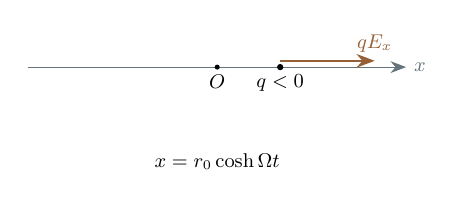
\begin{tikzpicture}[scale=.8,transform shape]
\draw[axis] (-3,0)--(3,0) node[right] {$x$};\fill (0,0) circle(.04) node[below] {$O$};\fill (1,0) circle(.05) node[below] {$q<0$};\draw[force] (1,.1)--(2.5,.1) node[above] {$qE_x$};\node at (0,-1.5) {$x=r_0\cosh\Omega t$};
\end{tikzpicture}
\figcaption{变图电试2.1V1\quad 负电荷在桌面内沿偏离中心的方向加速}
\end{minipage}\end{center}

\Needspace{20\baselineskip}
\item 正电小球从$(r_0,0)$释放时另给初速度$u_0\hat y$，求线性近似中的轨迹。
\textbf{解：}变图电试2.1V2中两个面内方向具有相同频率$\omega$，初值给$x=r_0\cos\omega t$、$y=(u_0/\omega)\sin\omega t$。因此轨迹是中心位于$O$、半轴为$r_0$和$|u_0|/\omega$的椭圆，角动量$L_z=mr_0u_0$保持不变。$u_0=0$时椭圆退化为直径；$|u_0|=\omega r_0$时为圆。一般初值则写成$x=A\cos\omega t+B\sin\omega t$、$y=C\cos\omega t+D\sin\omega t$，同样给中心椭圆。
\begin{center}\begin{minipage}{.98\linewidth}\centering
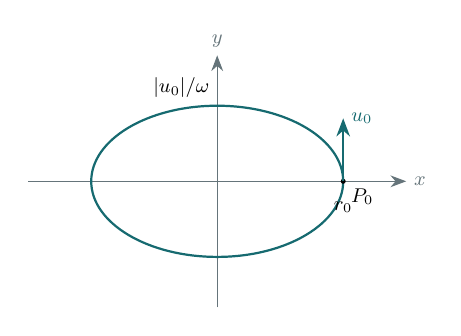
\begin{tikzpicture}[scale=.8,transform shape]
\draw[axis] (-3,0)--(3,0) node[right] {$x$};\draw[axis] (0,-2)--(0,2) node[above] {$y$};\draw[traj] (0,0) ellipse (2 and 1.2);\fill (2,0) circle(.04) node[below right] {$P_0$};\draw[motion] (2,0)--(2,1) node[right] {$u_0$};\node[below] at (2,-.2) {$r_0$};\node[above left] at (0,1.2) {$|u_0|/\omega$};
\end{tikzpicture}
\figcaption{变图电试2.1V2\quad 等频面内运动由静止释放的直径推广为中心椭圆}
\end{minipage}\end{center}

\Needspace{20\baselineskip}
\item 保留面内势能四次项，求静止释放振幅$r_0$的主要周期修正。
\textbf{解：}变图电试2.1V3从电势展开得到$\ddot x+\omega^2x+[9\omega^2/(8R^2)]x^3=0$。取$x\simeq r_0\cos\Omega t$，用$\cos^3\Omega t=(3\cos\Omega t+\cos3\Omega t)/4$，平衡基频项给$\Omega^2=\omega^2[1+27r_0^2/(32R^2)]$。开平方后$\Omega\simeq\omega[1+27r_0^2/(64R^2)]$，所以$T/T_0\simeq1-27r_0^2/(64R^2)$。四次势能项为正，恢复力随振幅变强，周期的主要修正为负。
\begin{center}\begin{minipage}{.98\linewidth}\centering
\begin{tikzpicture}[scale=.8,transform shape]
\draw[axis] (0,0)--(10.7,0) node[right] {$r_0/R$};
\draw[axis] (0,0)--(0,3.2) node[above] {$T/T_0$};\foreach \y/\lab in {0/.98,1.4/.99,2.8/1}{\draw[thin] (0,\y)--(-.08,\y) node[left] {$\lab$};}
\node[above] at (5,3.5) {四次势能给振幅平方阶的周期缩短};
\draw[traj] plot coordinates {(0.000000000,2.800000000) (0.100000000,2.799763750) (0.200000000,2.799055000) (0.300000000,2.797873750) (0.400000000,2.796220000) (0.500000000,2.794093750) (0.600000000,2.791495000) (0.700000000,2.788423750) (0.800000000,2.784880000) (0.900000000,2.780863750) (1.000000000,2.776375000) (1.100000000,2.771413750) (1.200000000,2.765980000) (1.300000000,2.760073750) (1.400000000,2.753695000) (1.500000000,2.746843750) (1.600000000,2.739520000) (1.700000000,2.731723750) (1.800000000,2.723455000) (1.900000000,2.714713750) (2.000000000,2.705500000) (2.100000000,2.695813750) (2.200000000,2.685655000) (2.300000000,2.675023750) (2.400000000,2.663920000) (2.500000000,2.652343750) (2.600000000,2.640295000) (2.700000000,2.627773750) (2.800000000,2.614780000) (2.900000000,2.601313750) (3.000000000,2.587375000) (3.100000000,2.572963750) (3.200000000,2.558080000) (3.300000000,2.542723750) (3.400000000,2.526895000) (3.500000000,2.510593750) (3.600000000,2.493820000) (3.700000000,2.476573750) (3.800000000,2.458855000) (3.900000000,2.440663750) (4.000000000,2.422000000) (4.100000000,2.402863750) (4.200000000,2.383255000) (4.300000000,2.363173750) (4.400000000,2.342620000) (4.500000000,2.321593750) (4.600000000,2.300095000) (4.700000000,2.278123750) (4.800000000,2.255680000) (4.900000000,2.232763750) (5.000000000,2.209375000) (5.100000000,2.185513750) (5.200000000,2.161180000) (5.300000000,2.136373750) (5.400000000,2.111095000) (5.500000000,2.085343750) (5.600000000,2.059120000) (5.700000000,2.032423750) (5.800000000,2.005255000) (5.900000000,1.977613750) (6.000000000,1.949500000) (6.100000000,1.920913750) (6.200000000,1.891855000) (6.300000000,1.862323750) (6.400000000,1.832320000) (6.500000000,1.801843750) (6.600000000,1.770895000) (6.700000000,1.739473750) (6.800000000,1.707580000) (6.900000000,1.675213750) (7.000000000,1.642375000) (7.100000000,1.609063750) (7.200000000,1.575280000) (7.300000000,1.541023750) (7.400000000,1.506295000) (7.500000000,1.471093750) (7.600000000,1.435420000) (7.700000000,1.399273750) (7.800000000,1.362655000) (7.900000000,1.325563750) (8.000000000,1.288000000) (8.100000000,1.249963750) (8.200000000,1.211455000) (8.300000000,1.172473750) (8.400000000,1.133020000) (8.500000000,1.093093750) (8.600000000,1.052695000) (8.700000000,1.011823750) (8.800000000,0.970480000) (8.900000000,0.928663750) (9.000000000,0.886375000) (9.100000000,0.843613750) (9.200000000,0.800380000) (9.300000000,0.756673750) (9.400000000,0.712495000) (9.500000000,0.667843750) (9.600000000,0.622720000) (9.700000000,0.577123750) (9.800000000,0.531055000) (9.900000000,0.484513750) (10.000000000,0.437500000)};
\node[below] at (0,-.12) {$0$};
\node[below] at (5,-.12) {$0.1$};
\node[below] at (10,-.12) {$0.2$};
\end{tikzpicture}
\figcaption{变图电试2.1V3\quad 四次势能给振幅平方阶的周期缩短}
\end{minipage}\end{center}

\Needspace{20\baselineskip}
\item 沿$x$方向另接弱弹簧，劲度为$k$、平衡位置在$O$，求该方向的有效频率与稳定条件。
\textbf{解：}变图电试2.1V4中弹簧力为$-kx$，电场力为$-\lambda qx/(4\varepsilon_0R^2)$，所以$\omega_x^2=k/m+\lambda q/(4\varepsilon_0mR^2)$。正电荷时两恢复作用相加；负电荷时$k>|\lambda q|/(4\varepsilon_0R^2)$给正的$\omega_x^2$，等号处线性项为零，保留三次项后有$\ddot x=[9\Omega^2/(8R^2)]x^3$，力沿位移方向，平衡仍不稳定，其中$\Omega^2=|\lambda q|/(4\varepsilon_0mR^2)$。弹簧只沿$x$作用，另一个面内方向仍由电场决定；负电荷若要仅作上述$x$方向振动，可用直线导向限定运动。
\begin{center}\begin{minipage}{.98\linewidth}\centering
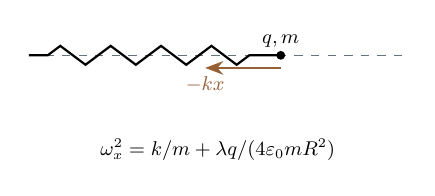
\begin{tikzpicture}[scale=.8,transform shape]
\draw[guide] (-3,0)--(3,0);\draw[thick] (-3,0)--(-2.7,0)--(-2.5,.15)--(-2.1,-.15)--(-1.7,.15)--(-1.3,-.15)--(-.9,.15)--(-.5,-.15)--(-.1,.15)--(.3,-.15)--(.5,0)--(1,0);\fill (1,0) circle(.07) node[above] {$q,m$};\draw[force] (1,-.2)--(-.2,-.2) node[below] {$-kx$};\node at (0,-1.5) {$\omega_x^2=k/m+\lambda q/(4\varepsilon_0mR^2)$};
\end{tikzpicture}
\figcaption{变图电试2.1V4\quad 机械弹簧和静电场在指定方向的刚度相加}
\end{minipage}\end{center}

\Needspace{20\baselineskip}
\item 改变环半径时，分别保持线电荷密度与总电荷不变，比较小振动周期的尺度。
\textbf{解：}变图电试2.1V5从$T=4\pi R\sqrt{\varepsilon_0m/(\lambda q)}$得到固定$\lambda$时$T\propto R$。若固定总电荷$Q=2\pi R\lambda$，代入$\lambda=Q/(2\pi R)$，得$T=4\pi\sqrt{2\pi\varepsilon_0mR^3/(Qq)}$，所以$T\propto R^{3/2}$。半径加倍时两种周期比分别为2和$2\sqrt2$。图中曲线按同一个参考半径归一化，体现改变半径时电荷条件也参与确定场梯度。
\begin{center}\begin{minipage}{.98\linewidth}\centering
\begin{tikzpicture}[scale=.8,transform shape]
\draw[axis] (0,0)--(10.7,0) node[right] {$R/R_*$ };
\draw[axis] (0,0)--(0,3.2) node[above] {$T/T_*$};
\node[above] at (5,3.5) {实线固定线密度，虚线固定总电荷};
\draw[traj] plot coordinates {(0.000000000,0.500000000) (0.083333333,0.512500000) (0.166666667,0.525000000) (0.250000000,0.537500000) (0.333333333,0.550000000) (0.416666667,0.562500000) (0.500000000,0.575000000) (0.583333333,0.587500000) (0.666666667,0.600000000) (0.750000000,0.612500000) (0.833333333,0.625000000) (0.916666667,0.637500000) (1.000000000,0.650000000) (1.083333333,0.662500000) (1.166666667,0.675000000) (1.250000000,0.687500000) (1.333333333,0.700000000) (1.416666667,0.712500000) (1.500000000,0.725000000) (1.583333333,0.737500000) (1.666666667,0.750000000) (1.750000000,0.762500000) (1.833333333,0.775000000) (1.916666667,0.787500000) (2.000000000,0.800000000) (2.083333333,0.812500000) (2.166666667,0.825000000) (2.250000000,0.837500000) (2.333333333,0.850000000) (2.416666667,0.862500000) (2.500000000,0.875000000) (2.583333333,0.887500000) (2.666666667,0.900000000) (2.750000000,0.912500000) (2.833333333,0.925000000) (2.916666667,0.937500000) (3.000000000,0.950000000) (3.083333333,0.962500000) (3.166666667,0.975000000) (3.250000000,0.987500000) (3.333333333,1.000000000) (3.416666667,1.012500000) (3.500000000,1.025000000) (3.583333333,1.037500000) (3.666666667,1.050000000) (3.750000000,1.062500000) (3.833333333,1.075000000) (3.916666667,1.087500000) (4.000000000,1.100000000) (4.083333333,1.112500000) (4.166666667,1.125000000) (4.250000000,1.137500000) (4.333333333,1.150000000) (4.416666667,1.162500000) (4.500000000,1.175000000) (4.583333333,1.187500000) (4.666666667,1.200000000) (4.750000000,1.212500000) (4.833333333,1.225000000) (4.916666667,1.237500000) (5.000000000,1.250000000) (5.083333333,1.262500000) (5.166666667,1.275000000) (5.250000000,1.287500000) (5.333333333,1.300000000) (5.416666667,1.312500000) (5.500000000,1.325000000) (5.583333333,1.337500000) (5.666666667,1.350000000) (5.750000000,1.362500000) (5.833333333,1.375000000) (5.916666667,1.387500000) (6.000000000,1.400000000) (6.083333333,1.412500000) (6.166666667,1.425000000) (6.250000000,1.437500000) (6.333333333,1.450000000) (6.416666667,1.462500000) (6.500000000,1.475000000) (6.583333333,1.487500000) (6.666666667,1.500000000) (6.750000000,1.512500000) (6.833333333,1.525000000) (6.916666667,1.537500000) (7.000000000,1.550000000) (7.083333333,1.562500000) (7.166666667,1.575000000) (7.250000000,1.587500000) (7.333333333,1.600000000) (7.416666667,1.612500000) (7.500000000,1.625000000) (7.583333333,1.637500000) (7.666666667,1.650000000) (7.750000000,1.662500000) (7.833333333,1.675000000) (7.916666667,1.687500000) (8.000000000,1.700000000) (8.083333333,1.712500000) (8.166666667,1.725000000) (8.250000000,1.737500000) (8.333333333,1.750000000) (8.416666667,1.762500000) (8.500000000,1.775000000) (8.583333333,1.787500000) (8.666666667,1.800000000) (8.750000000,1.812500000) (8.833333333,1.825000000) (8.916666667,1.837500000) (9.000000000,1.850000000) (9.083333333,1.862500000) (9.166666667,1.875000000) (9.250000000,1.887500000) (9.333333333,1.900000000) (9.416666667,1.912500000) (9.500000000,1.925000000) (9.583333333,1.937500000) (9.666666667,1.950000000) (9.750000000,1.962500000) (9.833333333,1.975000000) (9.916666667,1.987500000) (10.000000000,2.000000000)};
\draw[dashed,thick,color=warm] plot coordinates {(0.000000000,0.353553391) (0.083333333,0.366894165) (0.166666667,0.380398640) (0.250000000,0.394064854) (0.333333333,0.407890917) (0.416666667,0.421875000) (0.500000000,0.436015338) (0.583333333,0.450310223) (0.666666667,0.464758002) (0.750000000,0.479357073) (0.833333333,0.494105884) (0.916666667,0.509002932) (1.000000000,0.524046754) (1.083333333,0.539235932) (1.166666667,0.554569089) (1.250000000,0.570044886) (1.333333333,0.585662019) (1.416666667,0.601419220) (1.500000000,0.617315256) (1.583333333,0.633348924) (1.666666667,0.649519053) (1.750000000,0.665824501) (1.833333333,0.682264153) (1.916666667,0.698836924) (2.000000000,0.715541753) (2.083333333,0.732377603) (2.166666667,0.749343463) (2.250000000,0.766438343) (2.333333333,0.783661279) (2.416666667,0.801011324) (2.500000000,0.818487553) (2.583333333,0.836089063) (2.666666667,0.853814968) (2.750000000,0.871664401) (2.833333333,0.889636513) (2.916666667,0.907730472) (3.000000000,0.925945463) (3.083333333,0.944280687) (3.166666667,0.962735361) (3.250000000,0.981308716) (3.333333333,1.000000000) (3.416666667,1.018808472) (3.500000000,1.037733407) (3.583333333,1.056774093) (3.666666667,1.075929830) (3.750000000,1.095199932) (3.833333333,1.114583723) (3.916666667,1.134080540) (4.000000000,1.153689733) (4.083333333,1.173410660) (4.166666667,1.193242693) (4.250000000,1.213185212) (4.333333333,1.233237609) (4.416666667,1.253399284) (4.500000000,1.273669649) (4.583333333,1.294048124) (4.666666667,1.314534138) (4.750000000,1.335127130) (4.833333333,1.355826547) (4.916666667,1.376631844) (5.000000000,1.397542486) (5.083333333,1.418557944) (5.166666667,1.439677698) (5.250000000,1.460901236) (5.333333333,1.482228053) (5.416666667,1.503657650) (5.500000000,1.525189537) (5.583333333,1.546823231) (5.666666667,1.568558255) (5.750000000,1.590394138) (5.833333333,1.612330417) (5.916666667,1.634366635) (6.000000000,1.656502339) (6.083333333,1.678737086) (6.166666667,1.701070435) (6.250000000,1.723501954) (6.333333333,1.746031214) (6.416666667,1.768657794) (6.500000000,1.791381276) (6.583333333,1.814201249) (6.666666667,1.837117307) (6.750000000,1.860129049) (6.833333333,1.883236078) (6.916666667,1.906438003) (7.000000000,1.929734438) (7.083333333,1.953125000) (7.166666667,1.976609313) (7.250000000,2.000187003) (7.333333333,2.023857703) (7.416666667,2.047621047) (7.500000000,2.071476677) (7.583333333,2.095424237) (7.666666667,2.119463375) (7.750000000,2.143593744) (7.833333333,2.167815000) (7.916666667,2.192126803) (8.000000000,2.216528818) (8.083333333,2.241020711) (8.166666667,2.265602155) (8.250000000,2.290272824) (8.333333333,2.315032397) (8.416666667,2.339880556) (8.500000000,2.364816986) (8.583333333,2.389841375) (8.666666667,2.414953416) (8.750000000,2.440152803) (8.833333333,2.465439236) (8.916666667,2.490812415) (9.000000000,2.516272044) (9.083333333,2.541817832) (9.166666667,2.567449488) (9.250000000,2.593166727) (9.333333333,2.618969263) (9.416666667,2.644856816) (9.500000000,2.670829108) (9.583333333,2.696885863) (9.666666667,2.723026809) (9.750000000,2.749251674) (9.833333333,2.775560191) (9.916666667,2.801952096) (10.000000000,2.828427125)};
\node[below] at (0,-.12) {$0.5$};
\node[below] at (3.3333333333333335,-.12) {$1$};
\node[below] at (10,-.12) {$2$};
\end{tikzpicture}
\figcaption{变图电试2.1V5\quad 实线固定线密度，虚线固定总电荷}
\end{minipage}\end{center}

\Needspace{20\baselineskip}
\item 撤去桌面的离面限制，取竖直向上为$z$轴。比较从$z=0$及$z=\delta z_0$静止释放的两条相邻轴向轨迹，求局部运动和轨迹间距。
\textbf{解：}变图电试2.1V6中，令$\omega_z^2=qa/m=2\omega^2$，由$E_z=az$和重力得$\ddot z=\omega_z^2z-g$。从$z=0$静止释放的参考轨迹为$z_{\rm ref}=g(1-\cosh\omega_zt)/\omega_z^2$；从$z=\delta z_0$静止释放的轨迹为$z=z_{\rm ref}+\delta z_0\cosh\omega_zt$。两式代回方程均满足初值，轨迹间距因此为$\delta z=z-z_{\rm ref}=\delta z_0\cosh(\sqrt2\omega t)$。图中画的是$\delta z/\delta z_0$；计算采用$|z_{\rm ref}|,|z|\ll R$的局部运动时间段。面内两个分量在同一局部近似中仍满足频率$\omega$的振动方程。三维局部电势为$V-V(0)=\lambda(x^2+y^2-2z^2)/(8\varepsilon_0R^2)$，两个正曲率与一个负曲率共同构成鞍点。桌面通过支持力保持$z=0$，本题的周期属于这个受限平面运动。
\begin{center}\begin{minipage}{.98\linewidth}\centering
\begin{tikzpicture}[scale=.8,transform shape]
\draw[axis] (0,0)--(10.7,0) node[right] {$\omega t$};
\draw[axis] (0,0)--(0,3.2) node[above] {$\delta z/\delta z_0$};\foreach \y/\lab in {0/1,1.4/5,2.8/9}{\draw[thin] (0,\y)--(-.08,\y) node[left] {$\lab$};}
\node[above] at (5,3.5) {失去离面约束时的轴向扰动增长};
\draw[traj] plot coordinates {(0.000000000,0.000000000) (0.083333333,0.000097227) (0.166666667,0.000388961) (0.250000000,0.000875365) (0.333333333,0.001556708) (0.416666667,0.002433370) (0.500000000,0.003505837) (0.583333333,0.004774706) (0.666666667,0.006240680) (0.750000000,0.007904576) (0.833333333,0.009767316) (0.916666667,0.011829936) (1.000000000,0.014093583) (1.083333333,0.016559512) (1.166666667,0.019229096) (1.250000000,0.022103816) (1.333333333,0.025185270) (1.416666667,0.028475170) (1.500000000,0.031975344) (1.583333333,0.035687736) (1.666666667,0.039614409) (1.750000000,0.043757545) (1.833333333,0.048119445) (1.916666667,0.052702532) (2.000000000,0.057509354) (2.083333333,0.062542580) (2.166666667,0.067805007) (2.250000000,0.073299558) (2.333333333,0.079029287) (2.416666667,0.084997377) (2.500000000,0.091207143) (2.583333333,0.097662035) (2.666666667,0.104365640) (2.750000000,0.111321682) (2.833333333,0.118534026) (2.916666667,0.126006679) (3.000000000,0.133743792) (3.083333333,0.141749663) (3.166666667,0.150028742) (3.250000000,0.158585628) (3.333333333,0.167425074) (3.416666667,0.176551992) (3.500000000,0.185971452) (3.583333333,0.195688688) (3.666666667,0.205709098) (3.750000000,0.216038250) (3.833333333,0.226681882) (3.916666667,0.237645908) (4.000000000,0.248936419) (4.083333333,0.260559687) (4.166666667,0.272522171) (4.250000000,0.284830517) (4.333333333,0.297491563) (4.416666667,0.310512343) (4.500000000,0.323900092) (4.583333333,0.337662246) (4.666666667,0.351806453) (4.750000000,0.366340570) (4.833333333,0.381272673) (4.916666667,0.396611057) (5.000000000,0.412364245) (5.083333333,0.428540987) (5.166666667,0.445150273) (5.250000000,0.462201329) (5.333333333,0.479703629) (5.416666667,0.497666896) (5.500000000,0.516101112) (5.583333333,0.535016517) (5.666666667,0.554423621) (5.750000000,0.574333205) (5.833333333,0.594756332) (5.916666667,0.615704348) (6.000000000,0.637188891) (6.083333333,0.659221897) (6.166666667,0.681815609) (6.250000000,0.704982578) (6.333333333,0.728735675) (6.416666667,0.753088098) (6.500000000,0.778053376) (6.583333333,0.803645379) (6.666666667,0.829878326) (6.750000000,0.856766791) (6.833333333,0.884325713) (6.916666667,0.912570404) (7.000000000,0.941516555) (7.083333333,0.971180248) (7.166666667,1.001577965) (7.250000000,1.032726592) (7.333333333,1.064643437) (7.416666667,1.097346231) (7.500000000,1.130853144) (7.583333333,1.165182791) (7.666666667,1.200354245) (7.750000000,1.236387047) (7.833333333,1.273301216) (7.916666667,1.311117261) (8.000000000,1.349856191) (8.083333333,1.389539530) (8.166666667,1.430189324) (8.250000000,1.471828158) (8.333333333,1.514479166) (8.416666667,1.558166043) (8.500000000,1.602913062) (8.583333333,1.648745082) (8.666666667,1.695687568) (8.750000000,1.743766600) (8.833333333,1.793008889) (8.916666667,1.843441794) (9.000000000,1.895093334) (9.083333333,1.947992206) (9.166666667,2.002167799) (9.250000000,2.057650213) (9.333333333,2.114470272) (9.416666667,2.172659544) (9.500000000,2.232250359) (9.583333333,2.293275824) (9.666666667,2.355769844) (9.750000000,2.419767138) (9.833333333,2.485303264) (9.916666667,2.552414630) (10.000000000,2.621138524)};
\node[below] at (0,-.12) {$0$};
\node[below] at (5,-.12) {$1$};
\node[below] at (10,-.12) {$2$};
\end{tikzpicture}
\figcaption{变图电试2.1V6\quad 失去离面约束时的轴向扰动增长}
\end{minipage}\end{center}

\Needspace{20\baselineskip}
\item 从完整环电势写出振幅$A<R$的直径振动周期积分，并说明转折点。
\textbf{解：}变图电试2.1V7设势能$\mathcal U(x)=qV(x)$，静止释放使总能量为$\mathcal U(A)$。能量给$\dot x^2=2[\mathcal U(A)-\mathcal U(x)]/m$，势能为偶函数，所以两转折点是$\pm A$。四分之一周期从0走到$A$，故$T(A)=4\sqrt{m/2}\int_0^A[\mathcal U(A)-\mathcal U(x)]^{-1/2}\mathrm dx$，其中$V(x)$用主解的完整角积分。令$\varphi(s)=(2\pi)^{-1}\int_0^{2\pi}(1-2s\cos\phi+s^2)^{-1/2}\mathrm d\phi$，则$T/T_0=\pi^{-1}\int_0^{A/R}[\varphi(A/R)-\varphi(s)]^{-1/2}\mathrm ds$。小振幅极限恢复$T_0$。
\begin{center}\begin{minipage}{.98\linewidth}\centering
\begin{tikzpicture}[scale=.8,transform shape]
\draw[axis] (0,0)--(10.7,0) node[right] {$x/R$};
\draw[axis] (0,0)--(0,3.2) node[above] {$[\mathcal U(x)-\mathcal U(0)]/(m\omega^2R^2)$};
\node[above] at (5,3.5) {能量水平线与偶势能曲线交于两个转折点};
\draw[traj] plot coordinates {(0.000000000,2.634677746) (0.071428571,2.554380932) (0.142857143,2.475585559) (0.214285714,2.398273883) (0.285714286,2.322428642) (0.357142857,2.248033048) (0.428571429,2.175070774) (0.500000000,2.103525938) (0.571428571,2.033383095) (0.642857143,1.964627222) (0.714285714,1.897243710) (0.785714286,1.831218350) (0.857142857,1.766537326) (0.928571429,1.703187201) (1.000000000,1.641154913) (1.071428571,1.580427760) (1.142857143,1.520993396) (1.214285714,1.462839819) (1.285714286,1.405955365) (1.357142857,1.350328699) (1.428571429,1.295948808) (1.500000000,1.242804992) (1.571428571,1.190886861) (1.642857143,1.140184324) (1.714285714,1.090687585) (1.785714286,1.042387134) (1.857142857,0.995273746) (1.928571429,0.949338469) (2.000000000,0.904572623) (2.071428571,0.860967794) (2.142857143,0.818515826) (2.214285714,0.777208819) (2.285714286,0.737039123) (2.357142857,0.697999335) (2.428571429,0.660082290) (2.500000000,0.623281063) (2.571428571,0.587588960) (2.642857143,0.552999517) (2.714285714,0.519506495) (2.785714286,0.487103877) (2.857142857,0.455785863) (2.928571429,0.425546869) (3.000000000,0.396381521) (3.071428571,0.368284657) (3.142857143,0.341251317) (3.214285714,0.315276745) (3.285714286,0.290356388) (3.357142857,0.266485888) (3.428571429,0.243661082) (3.500000000,0.221878003) (3.571428571,0.201132873) (3.642857143,0.181422102) (3.714285714,0.162742290) (3.785714286,0.145090220) (3.857142857,0.128462858) (3.928571429,0.112857354) (4.000000000,0.098271035) (4.071428571,0.084701411) (4.142857143,0.072146166) (4.214285714,0.060603161) (4.285714286,0.050070435) (4.357142857,0.040546197) (4.428571429,0.032028832) (4.500000000,0.024516896) (4.571428571,0.018009118) (4.642857143,0.012504396) (4.714285714,0.008001801) (4.785714286,0.004500570) (4.857142857,0.002000113) (4.928571429,0.000500007) (5.000000000,0.000000000) (5.071428571,0.000500007) (5.142857143,0.002000113) (5.214285714,0.004500570) (5.285714286,0.008001801) (5.357142857,0.012504396) (5.428571429,0.018009118) (5.500000000,0.024516896) (5.571428571,0.032028832) (5.642857143,0.040546197) (5.714285714,0.050070435) (5.785714286,0.060603161) (5.857142857,0.072146166) (5.928571429,0.084701411) (6.000000000,0.098271035) (6.071428571,0.112857354) (6.142857143,0.128462858) (6.214285714,0.145090220) (6.285714286,0.162742290) (6.357142857,0.181422102) (6.428571429,0.201132873) (6.500000000,0.221878003) (6.571428571,0.243661082) (6.642857143,0.266485888) (6.714285714,0.290356388) (6.785714286,0.315276745) (6.857142857,0.341251317) (6.928571429,0.368284657) (7.000000000,0.396381521) (7.071428571,0.425546869) (7.142857143,0.455785863) (7.214285714,0.487103877) (7.285714286,0.519506495) (7.357142857,0.552999517) (7.428571429,0.587588960) (7.500000000,0.623281063) (7.571428571,0.660082290) (7.642857143,0.697999335) (7.714285714,0.737039123) (7.785714286,0.777208819) (7.857142857,0.818515826) (7.928571429,0.860967794) (8.000000000,0.904572623) (8.071428571,0.949338469) (8.142857143,0.995273746) (8.214285714,1.042387134) (8.285714286,1.090687585) (8.357142857,1.140184324) (8.428571429,1.190886861) (8.500000000,1.242804992) (8.571428571,1.295948808) (8.642857143,1.350328699) (8.714285714,1.405955365) (8.785714286,1.462839819) (8.857142857,1.520993396) (8.928571429,1.580427760) (9.000000000,1.641154913) (9.071428571,1.703187201) (9.142857143,1.766537326) (9.214285714,1.831218350) (9.285714286,1.897243710) (9.357142857,1.964627222) (9.428571429,2.033383095) (9.500000000,2.103525938) (9.571428571,2.175070774) (9.642857143,2.248033048) (9.714285714,2.322428642) (9.785714286,2.398273883) (9.857142857,2.475585559) (9.928571429,2.554380932) (10.000000000,2.634677746)};
\draw[dashed,thick,color=warm] plot coordinates {(0.000000000,1.897243710) (0.071428571,1.897243710) (0.142857143,1.897243710) (0.214285714,1.897243710) (0.285714286,1.897243710) (0.357142857,1.897243710) (0.428571429,1.897243710) (0.500000000,1.897243710) (0.571428571,1.897243710) (0.642857143,1.897243710) (0.714285714,1.897243710) (0.785714286,1.897243710) (0.857142857,1.897243710) (0.928571429,1.897243710) (1.000000000,1.897243710) (1.071428571,1.897243710) (1.142857143,1.897243710) (1.214285714,1.897243710) (1.285714286,1.897243710) (1.357142857,1.897243710) (1.428571429,1.897243710) (1.500000000,1.897243710) (1.571428571,1.897243710) (1.642857143,1.897243710) (1.714285714,1.897243710) (1.785714286,1.897243710) (1.857142857,1.897243710) (1.928571429,1.897243710) (2.000000000,1.897243710) (2.071428571,1.897243710) (2.142857143,1.897243710) (2.214285714,1.897243710) (2.285714286,1.897243710) (2.357142857,1.897243710) (2.428571429,1.897243710) (2.500000000,1.897243710) (2.571428571,1.897243710) (2.642857143,1.897243710) (2.714285714,1.897243710) (2.785714286,1.897243710) (2.857142857,1.897243710) (2.928571429,1.897243710) (3.000000000,1.897243710) (3.071428571,1.897243710) (3.142857143,1.897243710) (3.214285714,1.897243710) (3.285714286,1.897243710) (3.357142857,1.897243710) (3.428571429,1.897243710) (3.500000000,1.897243710) (3.571428571,1.897243710) (3.642857143,1.897243710) (3.714285714,1.897243710) (3.785714286,1.897243710) (3.857142857,1.897243710) (3.928571429,1.897243710) (4.000000000,1.897243710) (4.071428571,1.897243710) (4.142857143,1.897243710) (4.214285714,1.897243710) (4.285714286,1.897243710) (4.357142857,1.897243710) (4.428571429,1.897243710) (4.500000000,1.897243710) (4.571428571,1.897243710) (4.642857143,1.897243710) (4.714285714,1.897243710) (4.785714286,1.897243710) (4.857142857,1.897243710) (4.928571429,1.897243710) (5.000000000,1.897243710) (5.071428571,1.897243710) (5.142857143,1.897243710) (5.214285714,1.897243710) (5.285714286,1.897243710) (5.357142857,1.897243710) (5.428571429,1.897243710) (5.500000000,1.897243710) (5.571428571,1.897243710) (5.642857143,1.897243710) (5.714285714,1.897243710) (5.785714286,1.897243710) (5.857142857,1.897243710) (5.928571429,1.897243710) (6.000000000,1.897243710) (6.071428571,1.897243710) (6.142857143,1.897243710) (6.214285714,1.897243710) (6.285714286,1.897243710) (6.357142857,1.897243710) (6.428571429,1.897243710) (6.500000000,1.897243710) (6.571428571,1.897243710) (6.642857143,1.897243710) (6.714285714,1.897243710) (6.785714286,1.897243710) (6.857142857,1.897243710) (6.928571429,1.897243710) (7.000000000,1.897243710) (7.071428571,1.897243710) (7.142857143,1.897243710) (7.214285714,1.897243710) (7.285714286,1.897243710) (7.357142857,1.897243710) (7.428571429,1.897243710) (7.500000000,1.897243710) (7.571428571,1.897243710) (7.642857143,1.897243710) (7.714285714,1.897243710) (7.785714286,1.897243710) (7.857142857,1.897243710) (7.928571429,1.897243710) (8.000000000,1.897243710) (8.071428571,1.897243710) (8.142857143,1.897243710) (8.214285714,1.897243710) (8.285714286,1.897243710) (8.357142857,1.897243710) (8.428571429,1.897243710) (8.500000000,1.897243710) (8.571428571,1.897243710) (8.642857143,1.897243710) (8.714285714,1.897243710) (8.785714286,1.897243710) (8.857142857,1.897243710) (8.928571429,1.897243710) (9.000000000,1.897243710) (9.071428571,1.897243710) (9.142857143,1.897243710) (9.214285714,1.897243710) (9.285714286,1.897243710) (9.357142857,1.897243710) (9.428571429,1.897243710) (9.500000000,1.897243710) (9.571428571,1.897243710) (9.642857143,1.897243710) (9.714285714,1.897243710) (9.785714286,1.897243710) (9.857142857,1.897243710) (9.928571429,1.897243710) (10.000000000,1.897243710)};
\node[below] at (0.7142857142857143,-.12) {$-A/R$};
\node[below] at (5,-.12) {$0$};
\node[below] at (9.285714285714286,-.12) {$A/R$};
\end{tikzpicture}
\figcaption{变图电试2.1V7\quad 能量水平线与偶势能曲线交于两个转折点}
\end{minipage}\end{center}

\Needspace{20\baselineskip}
\item 环上电荷改为$\lambda(\phi)=\lambda_0[1+\epsilon\cos2\phi]$，$0<\epsilon<2/3$，求中心附近两个面内振动频率。
\textbf{解：}变图电试2.1V8的密度在$x$轴两端较大，中心电场仍由对径电荷相消。把库仑场对位置取一阶展开，$E_x=[\lambda_0/(4\pi\varepsilon_0R^2)]x\int_0^{2\pi}(1-3\cos^2\phi)(1+\epsilon\cos2\phi)\mathrm d\phi$，积分为$-\pi(1+3\epsilon/2)$；$y$方向相应为$-\pi(1-3\epsilon/2)$。所以$\omega_x^2=\omega_0^2(1+3\epsilon/2)$、$\omega_y^2=\omega_0^2(1-3\epsilon/2)$，$\omega_0^2=\lambda_0q/(4\varepsilon_0mR^2)$。所给范围内两个频率平方均为正，环的二次对称密度使平面两个方向的恢复刚度不同。
\begin{center}\begin{minipage}{.98\linewidth}\centering
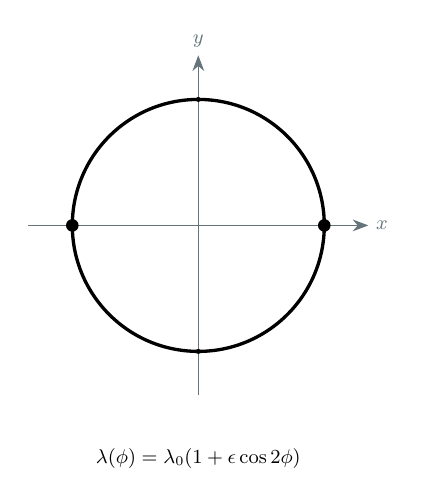
\begin{tikzpicture}[scale=.8,transform shape]
\draw[very thick] (0,0) circle (2);\draw[axis] (-2.7,0)--(2.7,0) node[right] {$x$};\draw[axis] (0,-2.7)--(0,2.7) node[above] {$y$};\fill (2,0) circle(.1);\fill (-2,0) circle(.1);\fill (0,2) circle(.04);\fill (0,-2) circle(.04);\node at (0,-3.7) {$\lambda(\phi)=\lambda_0(1+\epsilon\cos2\phi)$};
\end{tikzpicture}
\figcaption{变图电试2.1V8\quad $x$轴两侧较大的线密度改变两个方向的场梯度}
\end{minipage}\end{center}
\end{enumerate}

\Needspace{13\baselineskip}

\pdfbookmark[2]{第 2 题 圆锥曲线电流在焦点处的磁场}{q2}

\section*{第 2 题\quad 圆锥曲线电流在焦点处的磁场}\label{q:2}


用毕奥—萨伐尔定律求下列磁感应强度，电流均为稳恒电流$I$。
\begin{enumerate}
\item 椭圆闭合导线满足$x^2/A^2+y^2/B^2=1$，$A>B>0$。求焦点$F=(\sqrt{A^2-B^2},0)$处磁场大小$B_1$。
\item 在$x>0$的右支双曲线导线上，$x^2/A^2-y^2/B^2=1$，$A,B>0$，电流从上方无穷远沿右支流向下方无穷远。求内侧焦点$F=(\sqrt{A^2+B^2},0)$处磁场大小$B_2$。
\end{enumerate}
两导线均在纸面内；椭圆电流取逆时针。忽略连接到无穷远处的回路对有限位置的附加场。


\begin{center}\begin{minipage}{.98\linewidth}\centering
\begin{tikzpicture}[scale=.65,transform shape]

\draw[axis] (-3.1,0)--(3.1,0) node[right] {$x$};
\draw[axis] (0,-1.9)--(0,1.9) node[above] {$y$};
\draw[object] (0,0) ellipse (2.5 and 1.5);
\fill (2,0) circle (1.7pt) node[below right] {$F$};
\node[below left] at (0,0) {$O$};
\draw[motion] ({2.5*cos(30)},{1.5*sin(30)}) arc[start angle=30,end angle=65,x radius=2.5,y radius=1.5];
\node[above] at (1.5,1.5) {$I$};
\node at (0,-2.3) {椭圆：逆时针};
\begin{scope}[xshift=8cm]
\draw[axis] (-.5,0)--(3.7,0) node[right] {$x$};
\draw[axis] (0,-2.8)--(0,2.8) node[above] {$y$};
\draw[guide] (0,0)--(3.1,2.62307692);
\draw[guide] (0,0)--(3.1,-2.62307692);
\draw[object,domain=-1.6:1.6,samples=65] plot ({1.3*cosh(\x)},{1.1*sinh(\x)});
\fill (1.703,0) circle (1.7pt) node[below right] {$F$};
\node[below left] at (0,0) {$O$};
\draw[motion,domain=1.15:.8,samples=12] plot ({1.3*cosh(\x)},{1.1*sinh(\x)});
\node[left] at (1.65,1.4) {$I$};
\node at (1.6,-3.2) {右支：从上向下};
\end{scope}
\end{tikzpicture}
\figcaption{图电试2.2\quad 两条导线都在纸面内，分别求标记焦点处的场。}
\end{minipage}\end{center}

\Needspace{8\baselineskip}

\pdfbookmark[3]{题型定位}{q2-h0}

\subsection*{题型定位}

以焦点作极点，把平面曲线电流的毕奥—萨伐尔积分化为极角积分。先用矢量积去掉径向线元，再以圆锥曲线的倒半径表达式代入，使弧长积分转成常数与余弦的积分。两种曲线使用各自的正半径区间，电流方向同时决定极角增减与磁场正负。

\Needspace{8\baselineskip}

\pdfbookmark[3]{知识点}{q2-h1}

\subsection*{知识点}

电流元到焦点的位移是$-\boldsymbol r$，极坐标线元为$\mathrm dr\hat e_r+r\mathrm d\theta\hat e_\theta$。横向线元在矢量积中给$r^2\mathrm d\theta\hat z$，故场元正比于$\mathrm d\theta/r$。椭圆和双曲线的半通径都为$\ell=B^2/A$，偏心率分别小于1与大于1。无限支的角端点由渐近方向确定，倒半径在端点趋零。

\Needspace{8\baselineskip}

\pdfbookmark[3]{物理图像}{q2-h2}

\subsection*{物理图像}

题图的两个焦点均在电流曲线弯入的一侧，按所给电流方向，各场元均向纸外。解图电试2.2A将线元分解为径向与横向，图B标出双曲线从上端无穷远经顶点到下端无穷远的连续极角。图C用$1/r$的无量纲权重显示积分区间，两渐近端点处权重为零，顶点处最大。

\Needspace{8\baselineskip}

\pdfbookmark[3]{解题入口}{q2-h3}

\subsection*{解题入口}

暂时保留任意平面曲线，先推出$\mathrm dB_z=\mu_0I\mathrm d\theta/(4\pi r)$。再由焦点到顶点的距离决定极方程符号：椭圆右顶点在$\theta=0$，距离$A-c$；双曲线顶点在$\theta=\pi$，距离$c-A$。沿电流方向跟踪极角，确定连续变化的区间，把对应倒半径代入积分。

\Needspace{8\baselineskip}

\pdfbookmark[3]{标准解法}{q2-h4}

\subsection*{标准解法}


图电试2.2分别标出两条曲线及所求焦点。所有电流元都在纸面内，场点也在纸面内，因而每个磁场元均沿纸面法线。椭圆逆时针电流、双曲线上端至下端的电流，对所给焦点都产生向纸外的磁场。

以焦点$F$为极点、全局$+x$为极轴。令$\boldsymbol r=r\hat e_r$从$F$指向电流元，电流元到场点的矢量为$-\boldsymbol r$，则
\[
d\boldsymbol B=\frac{\mu_0I}{4\pi}
\frac{d\boldsymbol l\times(-\boldsymbol r)}{r^3}.
\]
\begin{center}\begin{minipage}{.98\linewidth}\centering
\begin{tikzpicture}[scale=.85,transform shape]

\fill (0,0) circle (1.7pt) node[below left] {$F$};
\draw[axis] (0,0)--(4.7,0) node[right] {极轴};
\draw[guide] (0,0)--(3,1.5) node[midway,above left] {$r$};
\draw[guide] (0,0)--(3.3,2.3);
\draw[object] (2.9,1.25) .. controls (3.05,1.6) and (3.18,2) .. (3.4,2.55);
\draw[motion] (3,1.5)--(3.3,2.3);
\draw[guide] (3.15,1.9)--(2.35,2.8) node[above] {$d\boldsymbol l$};
\draw[guide] (3,1.5)--(3.56,1.78)--(3.3,2.3);
\draw[force] (3,1.5)--(3.56,1.78);
\draw[motion] (3.56,1.78)--(3.3,2.3);
\node[right] at (3.6,1.3) {$dr\,\hat e_r$};
\node[above right] at (3.5,2.3) {$r\,d\theta\,\hat e_\theta$};
\draw[axis] (.9,.45) arc[start angle=26.565,end angle=34.875,radius=1.006];
\node at (1.3,.98) {$d\theta$};
\node at (1,-1) {$d\boldsymbol B\parallel+\hat z\quad\odot$};

\end{tikzpicture}
\figcaption{解图电试2.2A\quad 径向线元与位置矢量平行，横向投影决定磁场。}
\end{minipage}\end{center}
解图电试2.2A把$d\boldsymbol l$分成径向的$dr\,\hat e_r$与横向的$r\,d\theta\,\hat e_\theta$。径向部分无贡献，且
\[
d\boldsymbol l\times(-\boldsymbol r)
=r^2d\theta\,\hat z,\qquad
\boxed{dB_z=\frac{\mu_0I}{4\pi r}\,d\theta}.
\]
完整线元同时包含径向变化与横向变化，进入叉积的横向投影为$r\,d\theta$。

若线元的径向变化很大，完整弧长仍可很长，但径向分量与$-\boldsymbol r$平行，叉积恰为零。横向位移对应焦点所见的转角，因此场元由该转角与距离共同决定。沿所给电流方向$\mathrm d\theta>0$，$r>0$，所以这里可以将每个正的$B_z$贡献相加。

第（1）问记$c=\sqrt{A^2-B^2}$、$e=c/A$、$\ell=B^2/A$。相对于右焦点的极方程为
\[
r=\frac{\ell}{1+e\cos\theta}.
\]
极方程的符号可由右顶点直接说明：$\theta=0$时$r=\ell/(1+e)=B^2/(A+c)=A-c$；$\theta=\pi$时$r=\ell/(1-e)=A+c$，分别是右焦点到近、远顶点的距离。$e<1$保证每个方向都有正的有限半径。沿整个椭圆$\theta$增加$2\pi$，故
\[
B_1=\frac{\mu_0I}{4\pi\ell}
\int_0^{2\pi}(1+e\cos\theta)\,d\theta
=\frac{\mu_0I}{2\ell}.
\]
因此
\[
\boxed{B_1=\frac{\mu_0IA}{2B^2}},
\]
方向向纸外。整周积分中常数项给$2\pi$，余弦的原函数为正弦，两端取值相同而相消。因而最终只保留半通径$\ell$，再用$\ell=B^2/A$还原给定几何长度。若把极轴取向左，极方程相应为$r=\ell/(1-e\cos\theta)$，整周余弦积分仍为零，结果相同。

第（2）问记$c=\sqrt{A^2+B^2}$、$e=c/A>1$，仍有$\ell=B^2/A$。右支相对于右焦点的极方程为
\[
r=\frac{\ell}{1-e\cos\theta}.
\]
\begin{center}\begin{minipage}{.98\linewidth}\centering
\begin{tikzpicture}[scale=.8,transform shape]

\draw[axis] (-.5,0)--(3.7,0) node[right] {$x$};
\draw[axis] (0,-2.8)--(0,2.8) node[above] {$y$};
\draw[guide] (0,0)--(3.1,2.62307692);
\draw[guide] (0,0)--(3.1,-2.62307692);
\draw[object,domain=-1.6:1.6,samples=65] plot ({1.3*cosh(\x)},{1.1*sinh(\x)});
\fill (1.703,0) circle (1.7pt) node[below right] {$F$};
\node[below left] at (0,0) {$O$};
\draw[motion,domain=1.15:.8,samples=12] plot ({1.3*cosh(\x)},{1.1*sinh(\x)});
\node[left] at (1.65,1.4) {$I$};
\node at (1.6,-3.2) {右支：从上向下};

\draw[force] (1.703,0)--(3.503,1.523);
\draw[force] (1.703,0)--(3.503,-1.523);
\draw[guide] (1.703,0)--(3.6,0);
\node at (2.8,.5) {$\theta_0$};
\node at (.7,-.6) {$\theta=\pi$};
\node[align=center] at (-2.1,0) {$\theta_0<\theta$\\$\theta<2\pi-\theta_0$};
\node at (1.6,3.5) {焦点向右的一段角域不经过曲线};

\end{tikzpicture}
\figcaption{解图电试2.2B\quad 远端视线趋于渐近方向，积分跨过顶点而不跨向右的空扇区。}
\end{minipage}\end{center}
对右支，$\theta=\pi$给$r=\ell/(1+e)=B^2/(A+c)=c-A$，对应焦点向左到顶点的距离。沿双曲线向任一无穷远端延伸时，$r\to\infty$，所以分母$1-e\cos\theta$趋零。由$\cos\theta_0=1/e=A/c$可得$\sin\theta_0=B/c$、$\tan\theta_0=B/A$。解图电试2.2B中两条渐近方向给
\[
\theta_0=\arctan\frac BA,\qquad
\theta_0<\theta<2\pi-\theta_0.
\]
顶点处$\theta=\pi$；右焦点向右的射线不交该支的有限部分，因此有限曲线对应的角区间由两条渐近方向夹定。\begin{center}\begin{minipage}{.98\linewidth}\centering
\begin{tikzpicture}[scale=.8,transform shape]
\draw[axis] (0,0)--(10.7,0) node[right] {$\theta$};
\draw[axis] (0,0)--(0,3.2) node[above] {$\ell/r$};
\node[above] at (5,3.5) {$A=B$：两渐近方向间的倒半径权重};
\draw[traj] plot coordinates {(0.000000000,-0.000000000) (0.083333333,0.048036935) (0.166666667,0.097850114) (0.250000000,0.149362729) (0.333333333,0.202495349) (0.416666667,0.257166050) (0.500000000,0.313290532) (0.583333333,0.370782256) (0.666666667,0.429552574) (0.750000000,0.489510865) (0.833333333,0.550564680) (0.916666667,0.612619876) (1.000000000,0.675580771) (1.083333333,0.739350281) (1.166666667,0.803830080) (1.250000000,0.868920745) (1.333333333,0.934521910) (1.416666667,1.000532422) (1.500000000,1.066850499) (1.583333333,1.133373883) (1.666666667,1.200000000) (1.750000000,1.266626117) (1.833333333,1.333149501) (1.916666667,1.399467578) (2.000000000,1.465478090) (2.083333333,1.531079255) (2.166666667,1.596169920) (2.250000000,1.660649719) (2.333333333,1.724419229) (2.416666667,1.787380124) (2.500000000,1.849435320) (2.583333333,1.910489135) (2.666666667,1.970447426) (2.750000000,2.029217744) (2.833333333,2.086709468) (2.916666667,2.142833950) (3.000000000,2.197504651) (3.083333333,2.250637271) (3.166666667,2.302149886) (3.250000000,2.351963065) (3.333333333,2.400000000) (3.416666667,2.446186622) (3.500000000,2.490451715) (3.583333333,2.532727025) (3.666666667,2.572947367) (3.750000000,2.611050723) (3.833333333,2.646978341) (3.916666667,2.680674824) (4.000000000,2.712088213) (4.083333333,2.741170072) (4.166666667,2.767875558) (4.250000000,2.792163494) (4.333333333,2.813996429) (4.416666667,2.833340698) (4.500000000,2.850166475) (4.583333333,2.864447814) (4.666666667,2.876162696) (4.750000000,2.885293056) (4.833333333,2.891824817) (4.916666667,2.895747906) (5.000000000,2.897056275) (5.083333333,2.895747906) (5.166666667,2.891824817) (5.250000000,2.885293056) (5.333333333,2.876162696) (5.416666667,2.864447814) (5.500000000,2.850166475) (5.583333333,2.833340698) (5.666666667,2.813996429) (5.750000000,2.792163494) (5.833333333,2.767875558) (5.916666667,2.741170072) (6.000000000,2.712088213) (6.083333333,2.680674824) (6.166666667,2.646978341) (6.250000000,2.611050723) (6.333333333,2.572947367) (6.416666667,2.532727025) (6.500000000,2.490451715) (6.583333333,2.446186622) (6.666666667,2.400000000) (6.750000000,2.351963065) (6.833333333,2.302149886) (6.916666667,2.250637271) (7.000000000,2.197504651) (7.083333333,2.142833950) (7.166666667,2.086709468) (7.250000000,2.029217744) (7.333333333,1.970447426) (7.416666667,1.910489135) (7.500000000,1.849435320) (7.583333333,1.787380124) (7.666666667,1.724419229) (7.750000000,1.660649719) (7.833333333,1.596169920) (7.916666667,1.531079255) (8.000000000,1.465478090) (8.083333333,1.399467578) (8.166666667,1.333149501) (8.250000000,1.266626117) (8.333333333,1.200000000) (8.416666667,1.133373883) (8.500000000,1.066850499) (8.583333333,1.000532422) (8.666666667,0.934521910) (8.750000000,0.868920745) (8.833333333,0.803830080) (8.916666667,0.739350281) (9.000000000,0.675580771) (9.083333333,0.612619876) (9.166666667,0.550564680) (9.250000000,0.489510865) (9.333333333,0.429552574) (9.416666667,0.370782256) (9.500000000,0.313290532) (9.583333333,0.257166050) (9.666666667,0.202495349) (9.750000000,0.149362729) (9.833333333,0.097850114) (9.916666667,0.048036935) (10.000000000,0.000000000)};
\node[below] at (0,-.12) {$\pi/4$};
\node[below] at (5,-.12) {$\pi$};
\node[below] at (10,-.12) {$7\pi/4$};
\end{tikzpicture}
\figcaption{解图电试2.2C\quad $A=B$：两渐近方向间的倒半径权重}
\end{minipage}\end{center}
图C以$A=B$示例：顶点在横轴中点$\theta=\pi$，那里$1/r$最大；两个角端点处权重为零。电流从上方无穷远向顶点流动时，极角从$\theta_0$增加到$\pi$，再到下方无穷远的$2\pi-\theta_0$。下端角用连续增加的整周角表示，使一条导线支对应单一连续区间。两端趋向无穷远时，$1/r$趋零，积分收敛。于是
\[
\begin{aligned}
B_2&=\frac{\mu_0I}{4\pi\ell}
\int_{\theta_0}^{2\pi-\theta_0}(1-e\cos\theta)\,d\theta\\
&=\frac{\mu_0I}{2\pi\ell}
\bigl(\pi-\theta_0+e\sin\theta_0\bigr).
\end{aligned}
\]
积分的常数项给$2(\pi-\theta_0)$，余弦项的两端正弦分别为$-\sin\theta_0$与$+\sin\theta_0$，所以余弦部分额外给$2e\sin\theta_0$。由$\sin\theta_0=B/c$，$e\sin\theta_0=B/A$，得到
\[
\boxed{B_2=\frac{\mu_0IA}{2\pi B^2}
\left(\pi-\arctan\frac BA+\frac BA\right)}.
\]
方向也向纸外。两问用$A,B$表示几何半轴长度，用$B_1,B_2$表示焦点处的磁感应强度。
从量纲看，括号中的角度与$B/A$均为无量纲量，前因子$\mu_0IA/B^2$具有磁感应强度量纲。将椭圆逐渐变圆，焦点回到圆心，$A=B=R$给$\mu_0I/(2R)$；双曲线的角区间则由自己的渐近线连续决定。两问通过同一个局部叉积关系归结到不同的曲线倒半径与角区间，几何对象、极轴和电流方向在每一步保持一致。



\Needspace{8\baselineskip}

\pdfbookmark[3]{关键洞察}{q2-h5}

\subsection*{关键洞察}

曲线弧长的径向变化在叉积中消失，真正留下的是横向投影$r\mathrm d\theta$。焦点坐标使$1/r$对余弦呈一次关系，所以两问都只需初等积分。椭圆覆盖整周，余弦项抵消；双曲线只覆盖由渐近线围出的角区间，余弦项留下非零端点贡献。

\Needspace{8\baselineskip}

\pdfbookmark[3]{易错点}{q2-h6}

\subsection*{易错点}

线元分解时将$r\mathrm d\theta$理解为横向投影，完整弧长还含径向变化。给定极点与极轴后，用顶点距离确定分母符号。双曲线由上端流向下端时，极角跨过$\pi$连续增加，下端写成$2\pi-\theta_0$。几何半轴$B$、焦距$c$、偏心率$e$、半通径$\ell$与磁场$B_1,B_2$各按定义代入。

\Needspace{8\baselineskip}

\pdfbookmark[3]{课堂讲解建议}{q2-h7}

\subsection*{课堂讲解建议}

先画焦点、顶点和一个电流元，让学生用右手法则判断场方向，再把线元的两个极坐标分量分别放入叉积。得到通式后，先代顶点角度算距离，再决定极方程的正负号，据此代入倒半径做积分。

双曲线沿电流方向逐点增加$\theta$，标出上渐近角、顶点角和下渐近角，使上下限能从图上读出。比较图C与椭圆的整周权重，说明余弦项为何在一问抵消、另一问保留。再取圆形极限和抛物线极限，联系熟悉的圆环中心场与无限曲线的有限角积分。

\Needspace{8\baselineskip}

\pdfbookmark[3]{变式训练}{q2-h8}

\subsection*{变式训练}

\begin{enumerate}
\Needspace{20\baselineskip}
\item 令椭圆趋于半径$R$的圆，求焦点场的极限。
\textbf{解：}变图电试2.2V1中两个焦点随$A\to B=R$合并到圆心，偏心率$e\to0$，半通径$\ell\to R$。场元通式变成$\mathrm dB_z=\mu_0I\mathrm d\theta/(4\pi R)$，整周积分给$B_1=\mu_0I/(2R)$。这与将$A=B=R$直接代入$\mu_0IA/(2B^2)$一致。径向距离此时为常量，线元本身就是横向线元，恢复熟悉的圆电流中心磁场。
\begin{center}\begin{minipage}{.98\linewidth}\centering
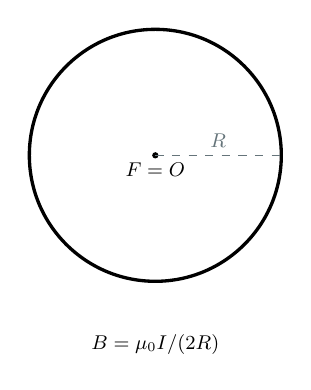
\begin{tikzpicture}[scale=.8,transform shape]
\draw[very thick] (0,0) circle (2);\fill (0,0) circle(.05) node[below] {$F=O$};\draw[guide] (0,0)--(2,0) node[midway,above] {$R$};\node at (0,-3) {$B=\mu_0I/(2R)$};
\end{tikzpicture}
\figcaption{变图电试2.2V1\quad 圆形极限中焦点合并为圆心}
\end{minipage}\end{center}

\Needspace{20\baselineskip}
\item 取右支双曲线$A=B$，求焦点磁场并写一个直角参数积分。
\textbf{解：}变图电试2.2V2中$c=\sqrt2A$、$e=\sqrt2$、$\ell=A$，渐近角为$\pi/4$，故$B_2=\mu_0I(3\pi/4+1)/(2\pi A)$。也可设$x=A\cosh u,y=A\sinh u$，电流由$u=+\infty$流向$-\infty$。叉积的正向大小为$A(c\cosh u-A)$，于是$B_2=[\mu_0I/(4\pi)]\int_{-\infty}^{\infty}A(c\cosh u-A)[(A\cosh u-c)^2+A^2\sinh^2u]^{-3/2}\mathrm du$，与极角结果描述同一条电流支。
\begin{center}\begin{minipage}{.98\linewidth}\centering
\begin{tikzpicture}[scale=.8,transform shape]
\draw[axis] (0,0)--(3,0) node[right] {$x/A$};\draw[axis] (0,-2.2)--(0,2.2) node[above] {$y/A$};\draw[guide] (0,0)--(2,2);\draw[guide] (0,0)--(2,-2);\draw[traj,domain=-1.3:1.3,samples=81] plot ({cosh(\x)},{sinh(\x)});\fill (1.414213562,0) circle(.04) node[below] {$F$};\node[above left] at (1,0) {顶点};\node at (1.5,-3) {$\theta_0=\pi/4$};
\end{tikzpicture}
\figcaption{变图电试2.2V2\quad 等半轴双曲线的顶点、焦点与渐近方向}
\end{minipage}\end{center}

\Needspace{20\baselineskip}
\item 只保留双曲线上$\theta_a$到$\theta_b$的一段，求它对焦点的磁场。
\textbf{解：}变图电试2.2V3取$\theta_0<\theta_a<\theta_b<2\pi-\theta_0$，电流沿极角增加方向。按同一通式积分，$B_z=\mu_0I[(\theta_b-\theta_a)-e(\sin\theta_b-\sin\theta_a)]/(4\pi\ell)$，为向纸外的正值。反向电流把符号反转。保留同一几何支的某段只改变积分限，极方程和横向投影保持原来的定义；连接段的附加场可按实际回路另行相加。
\begin{center}\begin{minipage}{.98\linewidth}\centering
\begin{tikzpicture}[scale=.8,transform shape]
\draw[axis] (0,0)--(10.7,0) node[right] {$\theta_b$};
\draw[axis] (0,0)--(0,3.2) node[above] {$4\pi\ell B_z/(\mu_0I)$};
\node[above] at (5,3.5) {$A=B,\theta_a=\pi/2$时逐段增加导线的磁场};
\draw[traj] plot coordinates {(0.000000000,0.000000000) (0.083333333,0.011999050) (0.166666667,0.024434104) (0.250000000,0.037304714) (0.333333333,0.050610134) (0.416666667,0.064349319) (0.500000000,0.078520927) (0.583333333,0.093123319) (0.666666667,0.108154561) (0.750000000,0.123612427) (0.833333333,0.139494396) (0.916666667,0.155797657) (1.000000000,0.172519112) (1.083333333,0.189655373) (1.166666667,0.207202772) (1.250000000,0.225157356) (1.333333333,0.243514893) (1.416666667,0.262270877) (1.500000000,0.281420527) (1.583333333,0.300958794) (1.666666667,0.320880360) (1.750000000,0.341179647) (1.833333333,0.361850816) (1.916666667,0.382887775) (2.000000000,0.404284179) (2.083333333,0.426033440) (2.166666667,0.448128725) (2.250000000,0.470562966) (2.333333333,0.493328861) (2.416666667,0.516418881) (2.500000000,0.539825277) (2.583333333,0.563540080) (2.666666667,0.587555111) (2.750000000,0.611861987) (2.833333333,0.636452122) (2.916666667,0.661316738) (3.000000000,0.686446867) (3.083333333,0.711833362) (3.166666667,0.737466897) (3.250000000,0.763337978) (3.333333333,0.789436950) (3.416666667,0.815753998) (3.500000000,0.842279161) (3.583333333,0.869002334) (3.666666667,0.895913276) (3.750000000,0.923001618) (3.833333333,0.950256869) (3.916666667,0.977668424) (4.000000000,1.005225570) (4.083333333,1.032917495) (4.166666667,1.060733294) (4.250000000,1.088661978) (4.333333333,1.116692481) (4.416666667,1.144813665) (4.500000000,1.173014331) (4.583333333,1.201283228) (4.666666667,1.229609054) (4.750000000,1.257980470) (4.833333333,1.286386107) (4.916666667,1.314814570) (5.000000000,1.343254450) (5.083333333,1.371694330) (5.166666667,1.400122794) (5.250000000,1.428528430) (5.333333333,1.456899847) (5.416666667,1.485225672) (5.500000000,1.513494569) (5.583333333,1.541695236) (5.666666667,1.569816420) (5.750000000,1.597846922) (5.833333333,1.625775606) (5.916666667,1.653591406) (6.000000000,1.681283331) (6.083333333,1.708840476) (6.166666667,1.736252031) (6.250000000,1.763507282) (6.333333333,1.790595624) (6.416666667,1.817506566) (6.500000000,1.844229739) (6.583333333,1.870754902) (6.666666667,1.897071951) (6.750000000,1.923170922) (6.833333333,1.949042004) (6.916666667,1.974675538) (7.000000000,2.000062033) (7.083333333,2.025192163) (7.166666667,2.050056778) (7.250000000,2.074646913) (7.333333333,2.098953789) (7.416666667,2.122968821) (7.500000000,2.146683624) (7.583333333,2.170090019) (7.666666667,2.193180040) (7.750000000,2.215945934) (7.833333333,2.238380175) (7.916666667,2.260475460) (8.000000000,2.282224721) (8.083333333,2.303621126) (8.166666667,2.324658084) (8.250000000,2.345329254) (8.333333333,2.365628540) (8.416666667,2.385550106) (8.500000000,2.405088373) (8.583333333,2.424238023) (8.666666667,2.442994007) (8.750000000,2.461351545) (8.833333333,2.479306128) (8.916666667,2.496853527) (9.000000000,2.513989789) (9.083333333,2.530711243) (9.166666667,2.547014504) (9.250000000,2.562896473) (9.333333333,2.578354339) (9.416666667,2.593385582) (9.500000000,2.607987973) (9.583333333,2.622159581) (9.666666667,2.635898766) (9.750000000,2.649204186) (9.833333333,2.662074797) (9.916666667,2.674509851) (10.000000000,2.686508900)};
\node[below] at (0,-.12) {$\pi/2$};
\node[below] at (5,-.12) {$\pi$};
\node[below] at (10,-.12) {$3\pi/2$};
\end{tikzpicture}
\figcaption{变图电试2.2V3\quad $A=B,\theta_a=\pi/2$时逐段增加导线的磁场}
\end{minipage}\end{center}

\Needspace{20\baselineskip}
\item 对完整抛物线支$r=\ell/(1+\cos\theta)$，求焦点处磁场，并用顶点焦距$f$表示。
\textbf{解：}变图电试2.2V4的焦点在原点，顶点在$\theta=0,r=\ell/2=f$，两端无穷远对应$\theta\to\pm\pi$。电流沿极角增加方向，$B_z=\mu_0I\int_{-\pi}^{\pi}(1+\cos\theta)\mathrm d\theta/(4\pi\ell)=\mu_0I/(2\ell)=\mu_0I/(4f)$，方向向纸外。两端虽然延伸无穷远，倒半径在角端点趋零，积分仍收敛。此式也由圆锥曲线焦点通式取偏心率$e=1$得到。
\begin{center}\begin{minipage}{.98\linewidth}\centering
\begin{tikzpicture}[scale=.8,transform shape]
\draw[axis] (-2,0)--(2,0) node[right] {$x$};\draw[axis] (0,-3)--(0,3) node[above] {$y$};\draw[traj,domain=-3:3,samples=81] plot ({1-\x*\x/4},\x);\fill (0,0) circle(.05) node[below left] {$F$};\fill (1,0) circle(.04) node[right] {顶点};\draw[<->] (0,-.5)--(1,-.5) node[midway,below] {$f=\ell/2$};
\end{tikzpicture}
\figcaption{变图电试2.2V4\quad 开口向左的完整抛物线，焦点在顶点左侧}
\end{minipage}\end{center}

\Needspace{20\baselineskip}
\item 一组椭圆保持半通径$\ell$和电流$I$相同，偏心率改变，问各自右焦点处磁场怎样变化。
\textbf{解：}变图电试2.2V5把每个椭圆的右焦点平移到共同极点，极方程为$r=\ell/(1+e\cos\theta)$。整周磁场$B_z=\mu_0I[\int_0^{2\pi}1\mathrm d\theta+e\int_0^{2\pi}\cos\theta\mathrm d\theta]/(4\pi\ell)=\mu_0I/(2\ell)$，与偏心率无关。曲线上不同方向的场贡献随形状重新分配，但余弦项的整周积分仍为零；比较的是每条椭圆各自焦点处的场。
\begin{center}\begin{minipage}{.98\linewidth}\centering
\begin{tikzpicture}[scale=.8,transform shape]
\draw[axis] (-2.5,0)--(1.7,0) node[right] {$x/\ell$};\draw[axis] (0,-1.8)--(0,1.8) node[above] {$y/\ell$};\draw[traj,domain=0:360,samples=121] plot ({cos(\x)},{sin(\x)});\draw[guide,domain=0:360,samples=121] plot ({cos(\x)/(1+.5*cos(\x))},{sin(\x)/(1+.5*cos(\x))});\fill (0,0) circle(.05) node[below right] {$F$};\node at (-.5,-2.7) {相同半通径$\ell$，不同偏心率};
\end{tikzpicture}
\figcaption{变图电试2.2V5\quad 焦点重合画出的椭圆族具有相同焦点场}
\end{minipage}\end{center}

\Needspace{20\baselineskip}
\item 将无限双曲线的两端同时在极角距渐近方向$\delta$处截断，其中$0<\delta<\pi-\theta_0$，求$\delta\ll1$时所漏磁场的主要阶次。
\textbf{解：}变图电试2.2V6中保留区间为$[\theta_0+\delta,2\pi-\theta_0-\delta]$。两端漏场相同，合计$\Delta B=\mu_0I\{\delta-e[\sin(\theta_0+\delta)-\sin\theta_0]\}/(2\pi\ell)$。由$e\cos\theta_0=1$，展开后一次项消失，得$\Delta B=\mu_0Ie\sin\theta_0\,\delta^2/(4\pi\ell)+O(\delta^3)$。倒半径在端点从零线性增长，故短角区间的面积为二阶小量，图中完整漏场与二次项在小$\delta$处接近。
\begin{center}\begin{minipage}{.98\linewidth}\centering
\begin{tikzpicture}[scale=.8,transform shape]
\draw[axis] (0,0)--(10.7,0) node[right] {$\delta$};
\draw[axis] (0,0)--(0,3.2) node[above] {$4\pi\ell\Delta B/(\mu_0I)$};
\node[above] at (5,3.5) {$A=B$：实线漏场，虚线二次主项};
\draw[traj] plot coordinates {(0.000000000,0.000000000) (0.083333333,0.000156380) (0.166666667,0.000626040) (0.250000000,0.001409759) (0.333333333,0.002508312) (0.416666667,0.003922475) (0.500000000,0.005653019) (0.583333333,0.007700715) (0.666666667,0.010066332) (0.750000000,0.012750636) (0.833333333,0.015754390) (0.916666667,0.019078359) (1.000000000,0.022723302) (1.083333333,0.026689978) (1.166666667,0.030979144) (1.250000000,0.035591553) (1.333333333,0.040527958) (1.416666667,0.045789109) (1.500000000,0.051375756) (1.583333333,0.057288643) (1.666666667,0.063528517) (1.750000000,0.070096118) (1.833333333,0.076992187) (1.916666667,0.084217462) (2.000000000,0.091772679) (2.083333333,0.099658573) (2.166666667,0.107875875) (2.250000000,0.116425315) (2.333333333,0.125307620) (2.416666667,0.134523518) (2.500000000,0.144073731) (2.583333333,0.153958980) (2.666666667,0.164179986) (2.750000000,0.174737466) (2.833333333,0.185632135) (2.916666667,0.196864706) (3.000000000,0.208435889) (3.083333333,0.220346396) (3.166666667,0.232596931) (3.250000000,0.245188199) (3.333333333,0.258120904) (3.416666667,0.271395745) (3.500000000,0.285013421) (3.583333333,0.298974628) (3.666666667,0.313280060) (3.750000000,0.327930409) (3.833333333,0.342926365) (3.916666667,0.358268614) (4.000000000,0.373957843) (4.083333333,0.389994734) (4.166666667,0.406379969) (4.250000000,0.423114227) (4.333333333,0.440198183) (4.416666667,0.457632513) (4.500000000,0.475417889) (4.583333333,0.493554981) (4.666666667,0.512044457) (4.750000000,0.530886982) (4.833333333,0.550083221) (4.916666667,0.569633834) (5.000000000,0.589539480) (5.083333333,0.609800816) (5.166666667,0.630418497) (5.250000000,0.651393175) (5.333333333,0.672725501) (5.416666667,0.694416121) (5.500000000,0.716465683) (5.583333333,0.738874829) (5.666666667,0.761644201) (5.750000000,0.784774438) (5.833333333,0.808266175) (5.916666667,0.832120048) (6.000000000,0.856336689) (6.083333333,0.880916728) (6.166666667,0.905860792) (6.250000000,0.931169507) (6.333333333,0.956843495) (6.416666667,0.982883378) (6.500000000,1.009289774) (6.583333333,1.036063300) (6.666666667,1.063204568) (6.750000000,1.090714191) (6.833333333,1.118592779) (6.916666667,1.146840937) (7.000000000,1.175459271) (7.083333333,1.204448384) (7.166666667,1.233808875) (7.250000000,1.263541341) (7.333333333,1.293646379) (7.416666667,1.324124582) (7.500000000,1.354976540) (7.583333333,1.386202842) (7.666666667,1.417804073) (7.750000000,1.449780818) (7.833333333,1.482133658) (7.916666667,1.514863172) (8.000000000,1.547969936) (8.083333333,1.581454526) (8.166666667,1.615317512) (8.250000000,1.649559465) (8.333333333,1.684180952) (8.416666667,1.719182537) (8.500000000,1.754564784) (8.583333333,1.790328252) (8.666666667,1.826473499) (8.750000000,1.863001080) (8.833333333,1.899911548) (8.916666667,1.937205455) (9.000000000,1.974883347) (9.083333333,2.012945771) (9.166666667,2.051393271) (9.250000000,2.090226386) (9.333333333,2.129445656) (9.416666667,2.169051617) (9.500000000,2.209044802) (9.583333333,2.249425743) (9.666666667,2.290194969) (9.750000000,2.331353006) (9.833333333,2.372900378) (9.916666667,2.414837606) (10.000000000,2.457165211)};
\draw[dashed,thick,color=warm] plot coordinates {(0.000000000,0.000000000) (0.083333333,0.000156250) (0.166666667,0.000625000) (0.250000000,0.001406250) (0.333333333,0.002500000) (0.416666667,0.003906250) (0.500000000,0.005625000) (0.583333333,0.007656250) (0.666666667,0.010000000) (0.750000000,0.012656250) (0.833333333,0.015625000) (0.916666667,0.018906250) (1.000000000,0.022500000) (1.083333333,0.026406250) (1.166666667,0.030625000) (1.250000000,0.035156250) (1.333333333,0.040000000) (1.416666667,0.045156250) (1.500000000,0.050625000) (1.583333333,0.056406250) (1.666666667,0.062500000) (1.750000000,0.068906250) (1.833333333,0.075625000) (1.916666667,0.082656250) (2.000000000,0.090000000) (2.083333333,0.097656250) (2.166666667,0.105625000) (2.250000000,0.113906250) (2.333333333,0.122500000) (2.416666667,0.131406250) (2.500000000,0.140625000) (2.583333333,0.150156250) (2.666666667,0.160000000) (2.750000000,0.170156250) (2.833333333,0.180625000) (2.916666667,0.191406250) (3.000000000,0.202500000) (3.083333333,0.213906250) (3.166666667,0.225625000) (3.250000000,0.237656250) (3.333333333,0.250000000) (3.416666667,0.262656250) (3.500000000,0.275625000) (3.583333333,0.288906250) (3.666666667,0.302500000) (3.750000000,0.316406250) (3.833333333,0.330625000) (3.916666667,0.345156250) (4.000000000,0.360000000) (4.083333333,0.375156250) (4.166666667,0.390625000) (4.250000000,0.406406250) (4.333333333,0.422500000) (4.416666667,0.438906250) (4.500000000,0.455625000) (4.583333333,0.472656250) (4.666666667,0.490000000) (4.750000000,0.507656250) (4.833333333,0.525625000) (4.916666667,0.543906250) (5.000000000,0.562500000) (5.083333333,0.581406250) (5.166666667,0.600625000) (5.250000000,0.620156250) (5.333333333,0.640000000) (5.416666667,0.660156250) (5.500000000,0.680625000) (5.583333333,0.701406250) (5.666666667,0.722500000) (5.750000000,0.743906250) (5.833333333,0.765625000) (5.916666667,0.787656250) (6.000000000,0.810000000) (6.083333333,0.832656250) (6.166666667,0.855625000) (6.250000000,0.878906250) (6.333333333,0.902500000) (6.416666667,0.926406250) (6.500000000,0.950625000) (6.583333333,0.975156250) (6.666666667,1.000000000) (6.750000000,1.025156250) (6.833333333,1.050625000) (6.916666667,1.076406250) (7.000000000,1.102500000) (7.083333333,1.128906250) (7.166666667,1.155625000) (7.250000000,1.182656250) (7.333333333,1.210000000) (7.416666667,1.237656250) (7.500000000,1.265625000) (7.583333333,1.293906250) (7.666666667,1.322500000) (7.750000000,1.351406250) (7.833333333,1.380625000) (7.916666667,1.410156250) (8.000000000,1.440000000) (8.083333333,1.470156250) (8.166666667,1.500625000) (8.250000000,1.531406250) (8.333333333,1.562500000) (8.416666667,1.593906250) (8.500000000,1.625625000) (8.583333333,1.657656250) (8.666666667,1.690000000) (8.750000000,1.722656250) (8.833333333,1.755625000) (8.916666667,1.788906250) (9.000000000,1.822500000) (9.083333333,1.856406250) (9.166666667,1.890625000) (9.250000000,1.925156250) (9.333333333,1.960000000) (9.416666667,1.995156250) (9.500000000,2.030625000) (9.583333333,2.066406250) (9.666666667,2.102500000) (9.750000000,2.138906250) (9.833333333,2.175625000) (9.916666667,2.212656250) (10.000000000,2.250000000)};
\node[below] at (0,-.12) {$0$};
\node[below] at (5,-.12) {$0.15$};
\node[below] at (10,-.12) {$0.3$};
\end{tikzpicture}
\figcaption{变图电试2.2V6\quad $A=B$：实线漏场，虚线二次主项}
\end{minipage}\end{center}

\Needspace{20\baselineskip}
\item 求椭圆上半环对右焦点的磁场，以及上半环两个极角象限各自的贡献。
\textbf{解：}变图电试2.2V7中上半环覆盖$0\le\theta\le\pi$，所以$B_{\rm upper}=\mu_0I\pi/(4\pi\ell)=\mu_0I/(4\ell)$，恰为整环的一半。靠近右顶点的角区间$0$到$\pi/2$贡献$\mu_0I(\pi/2+e)/(4\pi\ell)$，较远的$\pi/2$到$\pi$贡献$\mu_0I(\pi/2-e)/(4\pi\ell)$。两者之和保持不变，差别由倒半径中的余弦项控制，体现距离权重而非单纯弧长比例。
\begin{center}\begin{minipage}{.98\linewidth}\centering
\begin{tikzpicture}[scale=.8,transform shape]
\draw[axis] (0,0)--(10.7,0) node[right] {$\theta$};
\draw[axis] (0,0)--(0,3.2) node[above] {$\ell/r$};
\node[above] at (5,3.5) {$e=0.6$的上半环近侧、远侧权重};
\draw[traj] plot coordinates {(0.000000000,2.720000000) (0.083333333,2.719650471) (0.166666667,2.718602125) (0.250000000,2.716855680) (0.333333333,2.714412333) (0.416666667,2.711273759) (0.500000000,2.707442107) (0.583333333,2.702920006) (0.666666667,2.697710553) (0.750000000,2.691817319) (0.833333333,2.685244343) (0.916666667,2.677996130) (1.000000000,2.670077647) (1.083333333,2.661494321) (1.166666667,2.652252035) (1.250000000,2.642357123) (1.333333333,2.631816367) (1.416666667,2.620636990) (1.500000000,2.608826655) (1.583333333,2.596393455) (1.666666667,2.583345912) (1.750000000,2.569692968) (1.833333333,2.555443979) (1.916666667,2.540608712) (2.000000000,2.525197334) (2.083333333,2.509220407) (2.166666667,2.492688881) (2.250000000,2.475614085) (2.333333333,2.458007722) (2.416666667,2.439881858) (2.500000000,2.421248917) (2.583333333,2.402121667) (2.666666667,2.382513218) (2.750000000,2.362437009) (2.833333333,2.341906799) (2.916666667,2.320936658) (3.000000000,2.299540957) (3.083333333,2.277734362) (3.166666667,2.255531816) (3.250000000,2.232948536) (3.333333333,2.210000000) (3.416666667,2.186701935) (3.500000000,2.163070310) (3.583333333,2.139121319) (3.666666667,2.114871376) (3.750000000,2.090337101) (3.833333333,2.065535309) (3.916666667,2.040482996) (4.000000000,2.015197334) (4.083333333,1.989695652) (4.166666667,1.963995426) (4.250000000,1.938114271) (4.333333333,1.912069925) (4.416666667,1.885880236) (4.500000000,1.859563154) (4.583333333,1.833136716) (4.666666667,1.806619033) (4.750000000,1.780028278) (4.833333333,1.753382675) (4.916666667,1.726700487) (5.000000000,1.700000000) (5.083333333,1.673299513) (5.166666667,1.646617325) (5.250000000,1.619971722) (5.333333333,1.593380967) (5.416666667,1.566863284) (5.500000000,1.540436846) (5.583333333,1.514119764) (5.666666667,1.487930075) (5.750000000,1.461885729) (5.833333333,1.436004574) (5.916666667,1.410304348) (6.000000000,1.384802666) (6.083333333,1.359517004) (6.166666667,1.334464691) (6.250000000,1.309662899) (6.333333333,1.285128624) (6.416666667,1.260878681) (6.500000000,1.236929690) (6.583333333,1.213298065) (6.666666667,1.190000000) (6.750000000,1.167051464) (6.833333333,1.144468184) (6.916666667,1.122265638) (7.000000000,1.100459043) (7.083333333,1.079063342) (7.166666667,1.058093201) (7.250000000,1.037562991) (7.333333333,1.017486782) (7.416666667,0.997878333) (7.500000000,0.978751083) (7.583333333,0.960118142) (7.666666667,0.941992278) (7.750000000,0.924385915) (7.833333333,0.907311119) (7.916666667,0.890779593) (8.000000000,0.874802666) (8.083333333,0.859391288) (8.166666667,0.844556021) (8.250000000,0.830307032) (8.333333333,0.816654088) (8.416666667,0.803606545) (8.500000000,0.791173345) (8.583333333,0.779363010) (8.666666667,0.768183633) (8.750000000,0.757642877) (8.833333333,0.747747965) (8.916666667,0.738505679) (9.000000000,0.729922353) (9.083333333,0.722003870) (9.166666667,0.714755657) (9.250000000,0.708182681) (9.333333333,0.702289447) (9.416666667,0.697079994) (9.500000000,0.692557893) (9.583333333,0.688726241) (9.666666667,0.685587667) (9.750000000,0.683144320) (9.833333333,0.681397875) (9.916666667,0.680349529) (10.000000000,0.680000000)};
\node[below] at (0,-.12) {$0$};
\node[below] at (5,-.12) {$\pi/2$};
\node[below] at (10,-.12) {$\pi$};
\end{tikzpicture}
\figcaption{变图电试2.2V7\quad $e=0.6$的上半环近侧、远侧权重}
\end{minipage}\end{center}

\Needspace{20\baselineskip}
\item 同一逆时针椭圆电流，在左右两个焦点的磁场是否相同？分别用焦点极坐标说明。
\textbf{解：}变图电试2.2V8中左右焦点到相应近顶点的距离均为$A-c$。右焦点配$+x$极轴时$r_R=\ell/(1+e\cos\theta)$，左焦点配同一全局极轴时$r_L=\ell/(1-e\cos\theta)$。两处各自的极角沿逆时针电流均增加整周，余弦项都积分为零，故两焦点均有$B_z=\mu_0I/(2\ell)$，方向向纸外。几何反射对称把近、远弧段对调，完整电流的场大小与方向保持相同。
\begin{center}\begin{minipage}{.98\linewidth}\centering
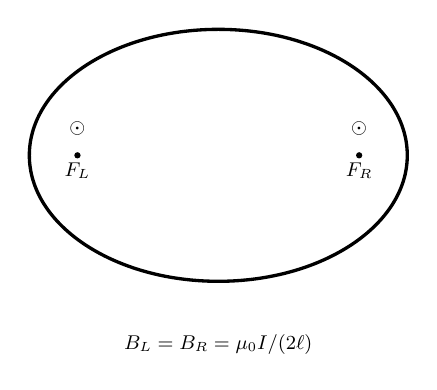
\begin{tikzpicture}[scale=.8,transform shape]
\draw[very thick] (0,0) ellipse (3 and 2);\fill (-2.236067978,0) circle(.05) node[below] {$F_L$};\fill (2.236067978,0) circle(.05) node[below] {$F_R$};\node[above] at (-2.236067978,.2) {$\odot$};\node[above] at (2.236067978,.2) {$\odot$};\node at (0,-3) {$B_L=B_R=\mu_0I/(2\ell)$};
\end{tikzpicture}
\figcaption{变图电试2.2V8\quad 左右焦点的整周余弦项都相消}
\end{minipage}\end{center}
\end{enumerate}

\Needspace{13\baselineskip}

\pdfbookmark[2]{第 3 题 磁力辅助的圆环外侧持续绕行}{q3}

\section*{第 3 题\quad 磁力辅助的圆环外侧持续绕行}\label{q:3}


半径$R$的固定光滑绝缘圆环位于竖直平面内。质量$m$、正电荷$Q$的质点从最高点$A$的外侧，以水平向左的速度$v_0>0$出发，空间中有垂直纸面向内的匀强磁场$B$，重力加速度为$g$。只有在圆环向外的支持力$N\ge0$时，质点才可沿外侧保持接触。
定义
\[
\lambda=\frac{v_0^2}{Rg}>0,\qquad
\mu=\frac{Q^2B^2R}{m^2g}>0.
\]
\begin{enumerate}
\item 假定质点能由$A$沿左半环到达最低点$B_{\rm p}$，并在该点恰好保持接触，求$\mu$与$\lambda$的关系。
\item 在这一关系下，证明最高点支持力为正。
\item 在这一关系下，求使左半环所有中间位置支持力均为正的全部$\lambda$。
\item 判断能否沿整个圆环持续绕行，并给出一般磁场强度下的保持接触条件。
\end{enumerate}
为区别最低点与磁感应强度，将最低点记为$B_{\rm p}$；忽略辐射和所有阻力。


\begin{center}\begin{minipage}{.98\linewidth}\centering
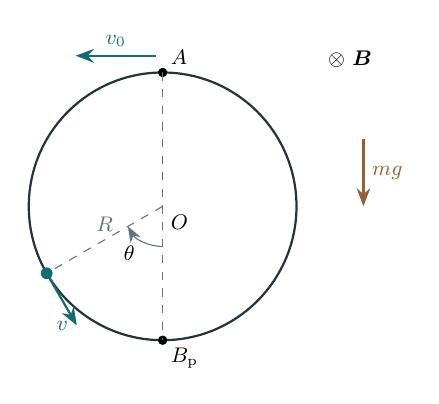
\begin{tikzpicture}[scale=.85,transform shape]

\draw[object] (0,0) circle (2);
\fill (0,2) circle (2pt) node[above right] {$A$};
\fill (0,-2) circle (2pt) node[below right] {$B_{\rm p}$};
\node[below right] at (0,0) {$O$};
\draw[guide] (0,2)--(0,-2);
\draw[motion] (-.1,2.25)--(-1.3,2.25) node[midway,above] {$v_0$};
\draw[guide] (0,0)--(-1.732,-1) node[midway,above] {$R$};
\fill[color=accent] (-1.732,-1) circle (2.5pt);
\draw[motion] (-1.732,-1)--(-1.282,-1.78) node[left] {$v$};
\draw[axis] (0,-.6) arc[start angle=-90,end angle=-150,radius=.6];
\node at (-.5,-.7) {$\theta$};
\draw[force] (3,1)--(3,0) node[midway,right] {$mg$};
\node at (2.8,2.2) {$\otimes\ \boldsymbol B$};

\end{tikzpicture}
\figcaption{图电试2.3\quad 质点沿左半环下降，磁力向心，圆环支持力向外。}
\end{minipage}\end{center}

\Needspace{8\baselineskip}

\pdfbookmark[3]{题型定位}{q3-h0}

\subsection*{题型定位}

带电质点受重力和洛伦兹力，圆环外侧接触由向外支持力$N\ge0$维持。先由能量求速度，再由径向方程求所需支持力，最后对整条路径判断这个支持力能否由圆环提供。最低点的临界等式确定参数关系，中间位置则由支持力函数的凹性和平方方法的符号区间证明。

\Needspace{8\baselineskip}

\pdfbookmark[3]{知识点}{q3-h1}

\subsection*{知识点}

洛伦兹力与速度垂直，光滑支持力与环切线垂直，两者都不作功。外侧圆环的支持力沿径向向外，给定磁场与绕行方向使磁力始终向内。无量纲化后支持力$n(c)$的二阶导数为负，最小值在最高、最低两端之一。处理含平方根的不等式先说明另一侧正负，最低点的孤立零支持力则结合邻域和速度连续性讨论。

\Needspace{8\baselineskip}

\pdfbookmark[3]{物理图像}{q3-h2}

\subsection*{物理图像}

解图电试2.3A的三个局部图分别标出最高点、一般点和最低点的力方向。重力径向投影随位置变号，磁力始终向心，支持力始终向外。图B以$c=\cos\theta$作横轴，用支持力曲线与端点弦线表示中间位置的正支持。图C在最低点两侧用带符号的小角表示同一个连续通过过程，支持力在一点为零，在两侧连续增为正。

\Needspace{8\baselineskip}

\pdfbookmark[3]{解题入口}{q3-h3}

\subsection*{解题入口}

由最高点到最低点的高度差$2R$先算$v_b$，再在最低点取$N_b=0$得到$\mu$与$\lambda$。随后在一般点统一取径向向外，把重力、磁力、支持力及径向加速度都写在同一方向约定中。将结果表示为$c$的函数，求二阶导数并连接两端点，便能控制全环各点的支持力。

\Needspace{8\baselineskip}

\pdfbookmark[3]{标准解法}{q3-h4}

\subsection*{标准解法}


图电试2.3中质点先沿左半环下降，磁力始终指向圆心，圆环支持力沿径向向外。设$\theta$为质点半径与竖直向下方向的夹角：$A$处$\theta=\pi$，$B_{\rm p}$处$\theta=0$，左半环上$\theta$随时间减小。

沿左半环可取位置$\boldsymbol r=(-R\sin\theta,-R\cos\theta)$，速度为$\boldsymbol v=(v\cos\theta,-v\sin\theta)$，其中$\dot\theta=-v/R$。磁场是$-B\hat z$，叉积$Q\boldsymbol v\times(-B\hat z)=QBv(\sin\theta,\cos\theta)$恰与位置矢量反向。最高点速度向左、最低点向右，磁力方向随切向速度连续转动，始终指向圆心。磁力和支持力都不做功，机械能守恒给
\[
\frac12mv^2=\frac12mv_0^2+mgR(1+\cos\theta),
\qquad
\boxed{\frac{v^2}{Rg}=\lambda+2+2\cos\theta}.
\]
最低点速度为$v_b=\sqrt{(\lambda+4)Rg}$。在最低点，磁力向上、重力和支持力向下，由向心方程
\[
\frac{mv_b^2}{R}=QBv_b-mg-N_b.
\]
最低点处向心方向向上。磁力提供向上的$QBv_b$，重力和外侧支持力都向下，故它们从可用向心合力中减去。$N_b$逐渐减到零时是本问指定的临界情况。第（1）问要求$N_b=0$，所以
\[
\lambda+4=\sqrt{\mu(\lambda+4)}-1,\qquad
\boxed{\mu=\frac{(\lambda+5)^2}{\lambda+4}}.
\]
质点下降时增加的动能全部来自重力势能的减少，磁力改变向心力的分配。
\begin{center}\begin{minipage}{.98\linewidth}\centering
\begin{tikzpicture}[scale=.68,transform shape]

\node at (0,2) {最高点 $A$};
\fill (0,0) circle (2.5pt);
\draw[force] (0,0)--(0,-1.2) node[right] {$QBv_0$};
\draw[force] (-.4,0)--(-.4,-.8) node[left] {$mg$};
\draw[force] (0,.2)--(0,1.2) node[right] {$N_A$};
\begin{scope}[xshift=4.5cm]
\node at (0,2) {一般位置};
\fill (0,0) circle (2.5pt);
\draw[guide] (-1.4,-.81)--(1.4,.81);
\draw[force] (0,0)--(1.04,.6) node[above right] {$QBv$};
\draw[force] (0,0)--(-1.04,-.6) node[below left] {$N$};
\draw[force] (0,-.1)--(0,-1.5) node[right] {$mg$};
\node at (0,-2.2) {向外：$mg\cos\theta-QBv+N$};
\end{scope}
\begin{scope}[xshift=9cm]
\node at (0,2) {最低点 $B_{\rm p}$};
\fill (0,0) circle (2.5pt);
\draw[force] (0,.1)--(0,1.25) node[right] {$QBv_b$};
\draw[force] (0,0)--(0,-1) node[right] {$mg$};
\node at (0,-1.7) {临界 $N_b=0$};
\end{scope}

\end{tikzpicture}
\figcaption{解图电试2.3A\quad 最高和最低位置的重力径向分量换号，磁力均向心。}
\end{minipage}\end{center}
解图电试2.3A分别画出最高、一般、最低位置的径向分量。取一般位置的径向向外为正，重力的向外分量为$mg\cos\theta$，磁力为$-QBv$，故
\[
-\frac{mv^2}{R}=mg\cos\theta-QBv+N.
\]
在一般点，$mg\cos\theta$在下半环向外、上半环向内；切向重力分量决定速率随位置怎样变化，径向重力分量则进入支持力方程。把能量得到的$v^2/(Rg)$和磁参数$QB/m=\sqrt{\mu g/R}$代入，磁力项化为$QBv/(mg)=\sqrt{\mu(\lambda+2+2\cos\theta)}$。于是令$c=\cos\theta$，
\[
\boxed{\frac N{mg}=n(c)
=\sqrt{\mu(\lambda+2+2c)}-(\lambda+2+3c)},
\qquad -1\le c\le1.
\]
最高点
\[
\frac{N_A}{mg}=\sqrt{\mu\lambda}-\lambda+1.
\]
若$0<\lambda\le1$，此式直接为正。若$\lambda>1$，需比较$\mu\lambda$与$(\lambda-1)^2$；代入临界关系，
\[
\mu\lambda-(\lambda-1)^2
=\frac{4(2\lambda^2+8\lambda-1)}{\lambda+4}>0.
\]
前一种情形中$1-\lambda\ge0$，再加正的磁项即为正。后一种情形只有在右侧$\lambda-1>0$时比较平方，代数差的分母$\lambda+4$为正，分子在$\lambda>1$也为正。因此第（2）问对所有$\lambda>0$均有$N_A>0$。

第（3）问还要把端点的正支持力条件延伸到全部中间位置。由
\[
n''(c)=-\frac{\sqrt\mu}{(\lambda+2+2c)^{3/2}}<0
\]
求导时$\lambda+2+2c\ge\lambda>0$，根号在整个闭区间内光滑，故二阶导数对每个位置都定义。可知$n$是凹函数，其图像位于连接两端点的弦线上方。临界关系下$n(1)=0$、$n(-1)>0$，故对$-1<c<1$，
\[
n(c)\ge\frac{1-c}{2}n(-1)>0.
\]
\begin{center}\begin{minipage}{.98\linewidth}\centering
\begin{tikzpicture}[scale=.8,transform shape]
\draw[axis] (0,0)--(10.7,0) node[right] {$c=\cos\theta$};
\draw[axis] (0,0)--(0,3.2) node[above] {$N/(mg)$};
\node[above] at (5,3.5) {$\lambda=1$：实线支持力，虚线端点弦线};
\draw[traj] plot coordinates {(0.000000000,2.683281573) (0.062500000,2.679115541) (0.125000000,2.674545417) (0.187500000,2.669585549) (0.250000000,2.664249456) (0.312500000,2.658549894) (0.375000000,2.652498914) (0.437500000,2.646107914) (0.500000000,2.639387691) (0.562500000,2.632348481) (0.625000000,2.625000000) (0.687500000,2.617351482) (0.750000000,2.609411708) (0.812500000,2.601189042) (0.875000000,2.592691454) (0.937500000,2.583926545) (1.000000000,2.574901573) (1.062500000,2.565623476) (1.125000000,2.556098884) (1.187500000,2.546334147) (1.250000000,2.536335345) (1.312500000,2.526108305) (1.375000000,2.515658618) (1.437500000,2.504991648) (1.500000000,2.494112550) (1.562500000,2.483026275) (1.625000000,2.471737588) (1.687500000,2.460251071) (1.750000000,2.448571137) (1.812500000,2.436702037) (1.875000000,2.424647870) (1.937500000,2.412412586) (2.000000000,2.400000000) (2.062500000,2.387413792) (2.125000000,2.374657518) (2.187500000,2.361734614) (2.250000000,2.348648402) (2.312500000,2.335402094) (2.375000000,2.321998799) (2.437500000,2.308441527) (2.500000000,2.294733192) (2.562500000,2.280876618) (2.625000000,2.266874542) (2.687500000,2.252729618) (2.750000000,2.238444419) (2.812500000,2.224021443) (2.875000000,2.209463115) (2.937500000,2.194771787) (3.000000000,2.179949748) (3.062500000,2.164999219) (3.125000000,2.149922359) (3.187500000,2.134721269) (3.250000000,2.119397990) (3.312500000,2.103954509) (3.375000000,2.088392760) (3.437500000,2.072714626) (3.500000000,2.056921938) (3.562500000,2.041016483) (3.625000000,2.025000000) (3.687500000,2.008874184) (3.750000000,1.992640687) (3.812500000,1.976301121) (3.875000000,1.959857057) (3.937500000,1.943310028) (4.000000000,1.926661531) (4.062500000,1.909913024) (4.125000000,1.893065934) (4.187500000,1.876121651) (4.250000000,1.859081537) (4.312500000,1.841946918) (4.375000000,1.824719092) (4.437500000,1.807399328) (4.500000000,1.789988864) (4.562500000,1.772488914) (4.625000000,1.754900661) (4.687500000,1.737225266) (4.750000000,1.719463864) (4.812500000,1.701617562) (4.875000000,1.683687449) (4.937500000,1.665674586) (5.000000000,1.647580015) (5.062500000,1.629404756) (5.125000000,1.611149806) (5.187500000,1.592816142) (5.250000000,1.574404724) (5.312500000,1.555916490) (5.375000000,1.537352360) (5.437500000,1.518713235) (5.500000000,1.500000000) (5.562500000,1.481213521) (5.625000000,1.462354649) (5.687500000,1.443424217) (5.750000000,1.424423043) (5.812500000,1.405351929) (5.875000000,1.386211663) (5.937500000,1.367003018) (6.000000000,1.347726751) (6.062500000,1.328383607) (6.125000000,1.308974318) (6.187500000,1.289499600) (6.250000000,1.269960159) (6.312500000,1.250356687) (6.375000000,1.230689864) (6.437500000,1.210960358) (6.500000000,1.191168825) (6.562500000,1.171315910) (6.625000000,1.151402247) (6.687500000,1.131428460) (6.750000000,1.111395160) (6.812500000,1.091302950) (6.875000000,1.071152423) (6.937500000,1.050944159) (7.000000000,1.030678732) (7.062500000,1.010356705) (7.125000000,0.989978632) (7.187500000,0.969545058) (7.250000000,0.949056520) (7.312500000,0.928513544) (7.375000000,0.907916650) (7.437500000,0.887266350) (7.500000000,0.866563146) (7.562500000,0.845807533) (7.625000000,0.825000000) (7.687500000,0.804141026) (7.750000000,0.783231083) (7.812500000,0.762270637) (7.875000000,0.741260147) (7.937500000,0.720200065) (8.000000000,0.699090834) (8.062500000,0.677932893) (8.125000000,0.656726674) (8.187500000,0.635472603) (8.250000000,0.614171097) (8.312500000,0.592822571) (8.375000000,0.571427432) (8.437500000,0.549986080) (8.500000000,0.528498912) (8.562500000,0.506966317) (8.625000000,0.485388679) (8.687500000,0.463766379) (8.750000000,0.442099788) (8.812500000,0.420389277) (8.875000000,0.398635209) (8.937500000,0.376837941) (9.000000000,0.354997828) (9.062500000,0.333115219) (9.125000000,0.311190457) (9.187500000,0.289223882) (9.250000000,0.267215829) (9.312500000,0.245166629) (9.375000000,0.223076607) (9.437500000,0.200946086) (9.500000000,0.178775383) (9.562500000,0.156564811) (9.625000000,0.134314681) (9.687500000,0.112025297) (9.750000000,0.089696962) (9.812500000,0.067329972) (9.875000000,0.044924623) (9.937500000,0.022481203) (10.000000000,0.000000000)};
\draw[dashed,thick,color=warm] plot coordinates {(0.000000000,2.683281573) (0.062500000,2.666511063) (0.125000000,2.649740553) (0.187500000,2.632970044) (0.250000000,2.616199534) (0.312500000,2.599429024) (0.375000000,2.582658514) (0.437500000,2.565888004) (0.500000000,2.549117494) (0.562500000,2.532346985) (0.625000000,2.515576475) (0.687500000,2.498805965) (0.750000000,2.482035455) (0.812500000,2.465264945) (0.875000000,2.448494435) (0.937500000,2.431723926) (1.000000000,2.414953416) (1.062500000,2.398182906) (1.125000000,2.381412396) (1.187500000,2.364641886) (1.250000000,2.347871376) (1.312500000,2.331100867) (1.375000000,2.314330357) (1.437500000,2.297559847) (1.500000000,2.280789337) (1.562500000,2.264018827) (1.625000000,2.247248317) (1.687500000,2.230477808) (1.750000000,2.213707298) (1.812500000,2.196936788) (1.875000000,2.180166278) (1.937500000,2.163395768) (2.000000000,2.146625258) (2.062500000,2.129854749) (2.125000000,2.113084239) (2.187500000,2.096313729) (2.250000000,2.079543219) (2.312500000,2.062772709) (2.375000000,2.046002199) (2.437500000,2.029231690) (2.500000000,2.012461180) (2.562500000,1.995690670) (2.625000000,1.978920160) (2.687500000,1.962149650) (2.750000000,1.945379140) (2.812500000,1.928608631) (2.875000000,1.911838121) (2.937500000,1.895067611) (3.000000000,1.878297101) (3.062500000,1.861526591) (3.125000000,1.844756081) (3.187500000,1.827985572) (3.250000000,1.811215062) (3.312500000,1.794444552) (3.375000000,1.777674042) (3.437500000,1.760903532) (3.500000000,1.744133022) (3.562500000,1.727362513) (3.625000000,1.710592003) (3.687500000,1.693821493) (3.750000000,1.677050983) (3.812500000,1.660280473) (3.875000000,1.643509963) (3.937500000,1.626739454) (4.000000000,1.609968944) (4.062500000,1.593198434) (4.125000000,1.576427924) (4.187500000,1.559657414) (4.250000000,1.542886904) (4.312500000,1.526116395) (4.375000000,1.509345885) (4.437500000,1.492575375) (4.500000000,1.475804865) (4.562500000,1.459034355) (4.625000000,1.442263845) (4.687500000,1.425493336) (4.750000000,1.408722826) (4.812500000,1.391952316) (4.875000000,1.375181806) (4.937500000,1.358411296) (5.000000000,1.341640786) (5.062500000,1.324870277) (5.125000000,1.308099767) (5.187500000,1.291329257) (5.250000000,1.274558747) (5.312500000,1.257788237) (5.375000000,1.241017728) (5.437500000,1.224247218) (5.500000000,1.207476708) (5.562500000,1.190706198) (5.625000000,1.173935688) (5.687500000,1.157165178) (5.750000000,1.140394669) (5.812500000,1.123624159) (5.875000000,1.106853649) (5.937500000,1.090083139) (6.000000000,1.073312629) (6.062500000,1.056542119) (6.125000000,1.039771610) (6.187500000,1.023001100) (6.250000000,1.006230590) (6.312500000,0.989460080) (6.375000000,0.972689570) (6.437500000,0.955919060) (6.500000000,0.939148551) (6.562500000,0.922378041) (6.625000000,0.905607531) (6.687500000,0.888837021) (6.750000000,0.872066511) (6.812500000,0.855296001) (6.875000000,0.838525492) (6.937500000,0.821754982) (7.000000000,0.804984472) (7.062500000,0.788213962) (7.125000000,0.771443452) (7.187500000,0.754672942) (7.250000000,0.737902433) (7.312500000,0.721131923) (7.375000000,0.704361413) (7.437500000,0.687590903) (7.500000000,0.670820393) (7.562500000,0.654049883) (7.625000000,0.637279374) (7.687500000,0.620508864) (7.750000000,0.603738354) (7.812500000,0.586967844) (7.875000000,0.570197334) (7.937500000,0.553426824) (8.000000000,0.536656315) (8.062500000,0.519885805) (8.125000000,0.503115295) (8.187500000,0.486344785) (8.250000000,0.469574275) (8.312500000,0.452803765) (8.375000000,0.436033256) (8.437500000,0.419262746) (8.500000000,0.402492236) (8.562500000,0.385721726) (8.625000000,0.368951216) (8.687500000,0.352180706) (8.750000000,0.335410197) (8.812500000,0.318639687) (8.875000000,0.301869177) (8.937500000,0.285098667) (9.000000000,0.268328157) (9.062500000,0.251557647) (9.125000000,0.234787138) (9.187500000,0.218016628) (9.250000000,0.201246118) (9.312500000,0.184475608) (9.375000000,0.167705098) (9.437500000,0.150934588) (9.500000000,0.134164079) (9.562500000,0.117393569) (9.625000000,0.100623059) (9.687500000,0.083852549) (9.750000000,0.067082039) (9.812500000,0.050311529) (9.875000000,0.033541020) (9.937500000,0.016770510) (10.000000000,0.000000000)};
\node[below] at (0,-.12) {$-1$};
\node[below] at (5,-.12) {$0$};
\node[below] at (10,-.12) {$1$};
\end{tikzpicture}
\figcaption{解图电试2.3B\quad $\lambda=1$：实线支持力，虚线端点弦线}
\end{minipage}\end{center}
弦线在$c=-1$取$n(-1)$，在$c=1$取0，其内点值为$(1-c)n(-1)/2$。因为内点$c<1$且$n(-1)>0$，整条弦线在内部为正；凹函数又在弦线上方，正支持力因而覆盖每个中间角度。这一步把端点条件与连续轨迹之间的关系明确写出。

解图电试2.3B中的曲线只在最低点$c=1$与零轴相接；最高点及全部中间位置均为正。故所求全部范围为
\[
\boxed{\lambda>0}.
\]
平方方法进一步说明含平方根不等式的符号条件。若$\lambda+2+3c\le0$，正的平方根已使$n(c)>0$。若$\lambda+2+3c>0$，比较两边平方，差的分子为
\[
\begin{aligned}
D(c)&=(\lambda+5)^2(\lambda+2+2c)
-(\lambda+4)(\lambda+2+3c)^2\\
&=(1-c)\bigl[9(\lambda+4)c+(\lambda+2)(4\lambda+17)\bigr].
\end{aligned}
\]
因式$1-c$在中间位置为正，判断平方差便归结到方括号的符号。它是$c$的一次函数，系数$9(\lambda+4)>0$，因此取允许区间的最小$c$即可得到下界。当$\lambda\ge1$时，方括号在$c>-1$范围的下界为
$2(2\lambda^2+8\lambda-1)>0$。当$0<\lambda<1$时，可平方的前提要求$c>-(\lambda+2)/3$，方括号因而大于
$(\lambda+2)(\lambda+5)>0$。在上述两个符号区间内，全部中间位置都得到$N>0$。

第（4）问右半环速度沿环向上，但磁力仍向圆心，同一$N(c)$公式继续适用。回到$A$时恢复初速，之后重复运动。最低点只有孤立的$N=0$，两侧支持力均为正，质点可以保持接触并通过该点：
\[
n(\cos\theta)
=\frac{2\lambda+7}{2(\lambda+4)}\theta^2+O(\theta^4)
\quad(\theta\to0).
\]
\begin{center}\begin{minipage}{.98\linewidth}\centering
\begin{tikzpicture}[scale=.8,transform shape]
\draw[axis] (0,0)--(10.7,0) node[right] {$\theta$};
\draw[axis] (0,0)--(0,3.2) node[above] {$N/(mg)$};\foreach \y/\lab in {0/0,1/0.05,2/0.1}{\draw[thin] (0,\y)--(-.08,\y) node[left] {$\lab$};}
\node[above] at (5,3.5) {最低点附近的正支持力与二次主项};
\draw[traj] plot coordinates {(0.000000000,2.826608060) (0.083333333,2.734868162) (0.166666667,2.644557845) (0.250000000,2.555682743) (0.333333333,2.468248401) (0.416666667,2.382260273) (0.500000000,2.297723724) (0.583333333,2.214644026) (0.666666667,2.133026361) (0.750000000,2.052875818) (0.833333333,1.974197396) (0.916666667,1.896996000) (1.000000000,1.821276443) (1.083333333,1.747043447) (1.166666667,1.674301638) (1.250000000,1.603055552) (1.333333333,1.533309628) (1.416666667,1.465068213) (1.500000000,1.398335561) (1.583333333,1.333115829) (1.666666667,1.269413081) (1.750000000,1.207231288) (1.833333333,1.146574322) (1.916666667,1.087445963) (2.000000000,1.029849893) (2.083333333,0.973789702) (2.166666667,0.919268880) (2.250000000,0.866290823) (2.333333333,0.814858831) (2.416666667,0.764976107) (2.500000000,0.716645758) (2.583333333,0.669870792) (2.666666667,0.624654122) (2.750000000,0.580998564) (2.833333333,0.538906836) (2.916666667,0.498381558) (3.000000000,0.459425254) (3.083333333,0.422040347) (3.166666667,0.386229167) (3.250000000,0.351993942) (3.333333333,0.319336802) (3.416666667,0.288259781) (3.500000000,0.258764813) (3.583333333,0.230853733) (3.666666667,0.204528280) (3.750000000,0.179790090) (3.833333333,0.156640704) (3.916666667,0.135081563) (4.000000000,0.115114008) (4.083333333,0.096739281) (4.166666667,0.079958526) (4.250000000,0.064772788) (4.333333333,0.051183011) (4.416666667,0.039190041) (4.500000000,0.028794624) (4.583333333,0.019997408) (4.666666667,0.012798938) (4.750000000,0.007199664) (4.833333333,0.003199934) (4.916666667,0.000799996) (5.000000000,0.000000000) (5.083333333,0.000799996) (5.166666667,0.003199934) (5.250000000,0.007199664) (5.333333333,0.012798938) (5.416666667,0.019997408) (5.500000000,0.028794624) (5.583333333,0.039190041) (5.666666667,0.051183011) (5.750000000,0.064772788) (5.833333333,0.079958526) (5.916666667,0.096739281) (6.000000000,0.115114008) (6.083333333,0.135081563) (6.166666667,0.156640704) (6.250000000,0.179790090) (6.333333333,0.204528280) (6.416666667,0.230853733) (6.500000000,0.258764813) (6.583333333,0.288259781) (6.666666667,0.319336802) (6.750000000,0.351993942) (6.833333333,0.386229167) (6.916666667,0.422040347) (7.000000000,0.459425254) (7.083333333,0.498381558) (7.166666667,0.538906836) (7.250000000,0.580998564) (7.333333333,0.624654122) (7.416666667,0.669870792) (7.500000000,0.716645758) (7.583333333,0.764976107) (7.666666667,0.814858831) (7.750000000,0.866290823) (7.833333333,0.919268880) (7.916666667,0.973789702) (8.000000000,1.029849893) (8.083333333,1.087445963) (8.166666667,1.146574322) (8.250000000,1.207231288) (8.333333333,1.269413081) (8.416666667,1.333115829) (8.500000000,1.398335561) (8.583333333,1.465068213) (8.666666667,1.533309628) (8.750000000,1.603055552) (8.833333333,1.674301638) (8.916666667,1.747043447) (9.000000000,1.821276443) (9.083333333,1.896996000) (9.166666667,1.974197396) (9.250000000,2.052875818) (9.333333333,2.133026361) (9.416666667,2.214644026) (9.500000000,2.297723724) (9.583333333,2.382260273) (9.666666667,2.468248401) (9.750000000,2.555682743) (9.833333333,2.644557845) (9.916666667,2.734868162) (10.000000000,2.826608060)};
\draw[dashed,thick,color=warm] plot coordinates {(0.000000000,2.880000000) (0.083333333,2.784800000) (0.166666667,2.691200000) (0.250000000,2.599200000) (0.333333333,2.508800000) (0.416666667,2.420000000) (0.500000000,2.332800000) (0.583333333,2.247200000) (0.666666667,2.163200000) (0.750000000,2.080800000) (0.833333333,2.000000000) (0.916666667,1.920800000) (1.000000000,1.843200000) (1.083333333,1.767200000) (1.166666667,1.692800000) (1.250000000,1.620000000) (1.333333333,1.548800000) (1.416666667,1.479200000) (1.500000000,1.411200000) (1.583333333,1.344800000) (1.666666667,1.280000000) (1.750000000,1.216800000) (1.833333333,1.155200000) (1.916666667,1.095200000) (2.000000000,1.036800000) (2.083333333,0.980000000) (2.166666667,0.924800000) (2.250000000,0.871200000) (2.333333333,0.819200000) (2.416666667,0.768800000) (2.500000000,0.720000000) (2.583333333,0.672800000) (2.666666667,0.627200000) (2.750000000,0.583200000) (2.833333333,0.540800000) (2.916666667,0.500000000) (3.000000000,0.460800000) (3.083333333,0.423200000) (3.166666667,0.387200000) (3.250000000,0.352800000) (3.333333333,0.320000000) (3.416666667,0.288800000) (3.500000000,0.259200000) (3.583333333,0.231200000) (3.666666667,0.204800000) (3.750000000,0.180000000) (3.833333333,0.156800000) (3.916666667,0.135200000) (4.000000000,0.115200000) (4.083333333,0.096800000) (4.166666667,0.080000000) (4.250000000,0.064800000) (4.333333333,0.051200000) (4.416666667,0.039200000) (4.500000000,0.028800000) (4.583333333,0.020000000) (4.666666667,0.012800000) (4.750000000,0.007200000) (4.833333333,0.003200000) (4.916666667,0.000800000) (5.000000000,0.000000000) (5.083333333,0.000800000) (5.166666667,0.003200000) (5.250000000,0.007200000) (5.333333333,0.012800000) (5.416666667,0.020000000) (5.500000000,0.028800000) (5.583333333,0.039200000) (5.666666667,0.051200000) (5.750000000,0.064800000) (5.833333333,0.080000000) (5.916666667,0.096800000) (6.000000000,0.115200000) (6.083333333,0.135200000) (6.166666667,0.156800000) (6.250000000,0.180000000) (6.333333333,0.204800000) (6.416666667,0.231200000) (6.500000000,0.259200000) (6.583333333,0.288800000) (6.666666667,0.320000000) (6.750000000,0.352800000) (6.833333333,0.387200000) (6.916666667,0.423200000) (7.000000000,0.460800000) (7.083333333,0.500000000) (7.166666667,0.540800000) (7.250000000,0.583200000) (7.333333333,0.627200000) (7.416666667,0.672800000) (7.500000000,0.720000000) (7.583333333,0.768800000) (7.666666667,0.819200000) (7.750000000,0.871200000) (7.833333333,0.924800000) (7.916666667,0.980000000) (8.000000000,1.036800000) (8.083333333,1.095200000) (8.166666667,1.155200000) (8.250000000,1.216800000) (8.333333333,1.280000000) (8.416666667,1.344800000) (8.500000000,1.411200000) (8.583333333,1.479200000) (8.666666667,1.548800000) (8.750000000,1.620000000) (8.833333333,1.692800000) (8.916666667,1.767200000) (9.000000000,1.843200000) (9.083333333,1.920800000) (9.166666667,2.000000000) (9.250000000,2.080800000) (9.333333333,2.163200000) (9.416666667,2.247200000) (9.500000000,2.332800000) (9.583333333,2.420000000) (9.666666667,2.508800000) (9.750000000,2.599200000) (9.833333333,2.691200000) (9.916666667,2.784800000) (10.000000000,2.880000000)};
\node[below] at (0,-.12) {$-0.4$};
\node[below] at (5,-.12) {$0$};
\node[below] at (10,-.12) {$0.4$};
\end{tikzpicture}
\figcaption{解图电试2.3C\quad 最低点附近的正支持力与二次主项}
\end{minipage}\end{center}
图C把最低点左右两侧的小角画在同一坐标中，实线为完整支持力，虚线为二次主项。质点通过时$v_b>0$，位置和速度连续；支持力连续降到零再升起，其所需方向始终沿外法线，因此圆环可维持这一约束运动。取连续角从$\pi$经0减到$-\pi$，同一个位置公式覆盖右半环，叉积的向心磁力关系也继续成立。

一般$\mu$下，凹性说明全环的最小支持力出现在两个端点之一。最低点条件为
$\mu\ge(\lambda+5)^2/(\lambda+4)$；最高点在$\lambda\le1$时自动满足，$\lambda>1$时要求$\mu\ge(\lambda-1)^2/\lambda$，后者弱于最低点条件。当$\lambda>1$，两端场强阈值之差为$4(2\lambda^2+8\lambda-1)/[\lambda(\lambda+4)]>0$，所以最低点给出的要求较强；当$\lambda\le1$时最高点本已满足非负支持力。又因$n(c)$为凹函数，满足这两个端点条件就覆盖整个圆环。因此
\[
\boxed{\lambda>0,\qquad
\mu\ge\frac{(\lambda+5)^2}{\lambda+4}}
\]
是这一方向持续绕行的条件；若要求全环处处严格$N>0$，将第二个不等号改成$>$。$\lambda=0$对应最高点严格静止的初态，切向力恰为零，质点停留在这个平衡位置；$\lambda\to0^+$则始终保留非零初速，绕行所需时间随初速减小而增加。
磁场提供向内偏转，沿环速率由能量式确定。临界磁场下，重力在下降半环增加动能，在上升半环取回相同动能，质点回到最高点时速度大小、方向和机械能都恢复；均匀静磁场、固定光滑环和无阻力条件于是使下一周重复同一过程。接触期间的绕行时间由$\mathrm dt=R|\mathrm d\theta|/v$积分，初速很小时主要时间花在最高点附近，实际运动与严格静止初态因此有不同的时间行为。



\Needspace{8\baselineskip}

\pdfbookmark[3]{关键洞察}{q3-h5}

\subsection*{关键洞察}

圆环可以向外推质点，所求支持力为负时则要求圆环向内拉，实际接触状态随之改变。临界场在最低点给$N=0$，邻域支持力按正的角度平方增加，且通过速度为正，所以约束圆周运动可连续通过该点。全程速度由重力势能确定，磁场改变的是维持轨迹所需的向心力分配。

\Needspace{8\baselineskip}

\pdfbookmark[3]{易错点}{q3-h6}

\subsection*{易错点}

在最高、最低点都把外侧支持力画向外，磁力则按速度与向内磁场的叉积画向圆心。能量式只计重力势能变化，磁场强度进入径向方程。最高点的磁项是$\sqrt{\mu\lambda}$，含有初速的平方根。对平方不等式先分$\lambda+2+3c$的符号，正的一侧再比较平方。非零微小初速与严格静止分别对应缓慢启动和停在最高点平衡的两种初始条件。

\Needspace{8\baselineskip}

\pdfbookmark[3]{课堂讲解建议}{q3-h7}

\subsection*{课堂讲解建议}

先让学生在顶端、底端各画力图，再改写为统一的径向正方向，说明相同方程怎样给出两个端点。得到最低点临界关系后，追问中间位置的支持力如何确定，让学生对$n(c)$求二阶导数并写弦线不等式。

再选$0<\lambda<1$，用平方方法展示右侧为负时条件直接成立、右侧为正时怎样分解代数差。最后对最低点小角展开，说明速度连续、支持力非负与孤立零点可以同时成立。把一般磁场下的两个端点条件比较，求出整个圆环保持接触的磁场阈值，并讨论固定磁场允许的初速范围。

\Needspace{8\baselineskip}

\pdfbookmark[3]{变式训练}{q3-h8}

\subsection*{变式训练}

\begin{enumerate}
\Needspace{20\baselineskip}
\item 令$\lambda=1$并取最低点临界磁场，求最高点与左右侧点的支持力。
\textbf{解：}变图电试2.3V1中$\mu=(1+5)^2/(1+4)=36/5$。最高点$c=-1$给$N_A/(mg)=\sqrt{36/5}=6/\sqrt5$；左右侧点$c=0$给$N/(mg)=\sqrt{108/5}-3>0$；最低点$c=1$给零。完整曲线是$n(c)=\sqrt{(36/5)(3+2c)}-3-3c$，二阶导数为负，位于端点弦线上方，因此侧点及其余中间位置均保持正支持力。
\begin{center}\begin{minipage}{.98\linewidth}\centering
\begin{tikzpicture}[scale=.8,transform shape]
\draw[axis] (0,0)--(10.7,0) node[right] {$c$};
\draw[axis] (0,0)--(0,3.2) node[above] {$N/(mg)$};
\node[above] at (5,3.5) {$\lambda=1,\mu=36/5$的全环支持力};
\draw[traj] plot coordinates {(0.000000000,2.683281573) (0.062500000,2.679115541) (0.125000000,2.674545417) (0.187500000,2.669585549) (0.250000000,2.664249456) (0.312500000,2.658549894) (0.375000000,2.652498914) (0.437500000,2.646107914) (0.500000000,2.639387691) (0.562500000,2.632348481) (0.625000000,2.625000000) (0.687500000,2.617351482) (0.750000000,2.609411708) (0.812500000,2.601189042) (0.875000000,2.592691454) (0.937500000,2.583926545) (1.000000000,2.574901573) (1.062500000,2.565623476) (1.125000000,2.556098884) (1.187500000,2.546334147) (1.250000000,2.536335345) (1.312500000,2.526108305) (1.375000000,2.515658618) (1.437500000,2.504991648) (1.500000000,2.494112550) (1.562500000,2.483026275) (1.625000000,2.471737588) (1.687500000,2.460251071) (1.750000000,2.448571137) (1.812500000,2.436702037) (1.875000000,2.424647870) (1.937500000,2.412412586) (2.000000000,2.400000000) (2.062500000,2.387413792) (2.125000000,2.374657518) (2.187500000,2.361734614) (2.250000000,2.348648402) (2.312500000,2.335402094) (2.375000000,2.321998799) (2.437500000,2.308441527) (2.500000000,2.294733192) (2.562500000,2.280876618) (2.625000000,2.266874542) (2.687500000,2.252729618) (2.750000000,2.238444419) (2.812500000,2.224021443) (2.875000000,2.209463115) (2.937500000,2.194771787) (3.000000000,2.179949748) (3.062500000,2.164999219) (3.125000000,2.149922359) (3.187500000,2.134721269) (3.250000000,2.119397990) (3.312500000,2.103954509) (3.375000000,2.088392760) (3.437500000,2.072714626) (3.500000000,2.056921938) (3.562500000,2.041016483) (3.625000000,2.025000000) (3.687500000,2.008874184) (3.750000000,1.992640687) (3.812500000,1.976301121) (3.875000000,1.959857057) (3.937500000,1.943310028) (4.000000000,1.926661531) (4.062500000,1.909913024) (4.125000000,1.893065934) (4.187500000,1.876121651) (4.250000000,1.859081537) (4.312500000,1.841946918) (4.375000000,1.824719092) (4.437500000,1.807399328) (4.500000000,1.789988864) (4.562500000,1.772488914) (4.625000000,1.754900661) (4.687500000,1.737225266) (4.750000000,1.719463864) (4.812500000,1.701617562) (4.875000000,1.683687449) (4.937500000,1.665674586) (5.000000000,1.647580015) (5.062500000,1.629404756) (5.125000000,1.611149806) (5.187500000,1.592816142) (5.250000000,1.574404724) (5.312500000,1.555916490) (5.375000000,1.537352360) (5.437500000,1.518713235) (5.500000000,1.500000000) (5.562500000,1.481213521) (5.625000000,1.462354649) (5.687500000,1.443424217) (5.750000000,1.424423043) (5.812500000,1.405351929) (5.875000000,1.386211663) (5.937500000,1.367003018) (6.000000000,1.347726751) (6.062500000,1.328383607) (6.125000000,1.308974318) (6.187500000,1.289499600) (6.250000000,1.269960159) (6.312500000,1.250356687) (6.375000000,1.230689864) (6.437500000,1.210960358) (6.500000000,1.191168825) (6.562500000,1.171315910) (6.625000000,1.151402247) (6.687500000,1.131428460) (6.750000000,1.111395160) (6.812500000,1.091302950) (6.875000000,1.071152423) (6.937500000,1.050944159) (7.000000000,1.030678732) (7.062500000,1.010356705) (7.125000000,0.989978632) (7.187500000,0.969545058) (7.250000000,0.949056520) (7.312500000,0.928513544) (7.375000000,0.907916650) (7.437500000,0.887266350) (7.500000000,0.866563146) (7.562500000,0.845807533) (7.625000000,0.825000000) (7.687500000,0.804141026) (7.750000000,0.783231083) (7.812500000,0.762270637) (7.875000000,0.741260147) (7.937500000,0.720200065) (8.000000000,0.699090834) (8.062500000,0.677932893) (8.125000000,0.656726674) (8.187500000,0.635472603) (8.250000000,0.614171097) (8.312500000,0.592822571) (8.375000000,0.571427432) (8.437500000,0.549986080) (8.500000000,0.528498912) (8.562500000,0.506966317) (8.625000000,0.485388679) (8.687500000,0.463766379) (8.750000000,0.442099788) (8.812500000,0.420389277) (8.875000000,0.398635209) (8.937500000,0.376837941) (9.000000000,0.354997828) (9.062500000,0.333115219) (9.125000000,0.311190457) (9.187500000,0.289223882) (9.250000000,0.267215829) (9.312500000,0.245166629) (9.375000000,0.223076607) (9.437500000,0.200946086) (9.500000000,0.178775383) (9.562500000,0.156564811) (9.625000000,0.134314681) (9.687500000,0.112025297) (9.750000000,0.089696962) (9.812500000,0.067329972) (9.875000000,0.044924623) (9.937500000,0.022481203) (10.000000000,0.000000000)};
\node[below] at (0,-.12) {$A:-1$};
\node[below] at (5,-.12) {侧点$0$};
\node[below] at (10,-.12) {$B_{\rm p}:1$};
\end{tikzpicture}
\figcaption{变图电试2.3V1\quad $\lambda=1,\mu=36/5$的全环支持力}
\end{minipage}\end{center}

\Needspace{20\baselineskip}
\item 去掉磁场，求外侧运动何时首次失去接触，并说明全环绕行的可能性。
\textbf{解：}变图电试2.3V2中$\mu=0$，所需支持力为$N/(mg)=-\lambda-2-3c$。若$0<\lambda<1$，最高点支持力$mg(1-\lambda)>0$，下降至$c=-(\lambda+2)/3$时首次达到零，之后按自由抛体运动。若$\lambda=1$，接触阈值就在最高点；若$\lambda>1$，最高点已需负支持力。最低点始终有$N_b=-m(v_b^2/R+g)<0$，因此无磁场的外侧单面圆环无法维持本题的完整绕行。
\begin{center}\begin{minipage}{.98\linewidth}\centering
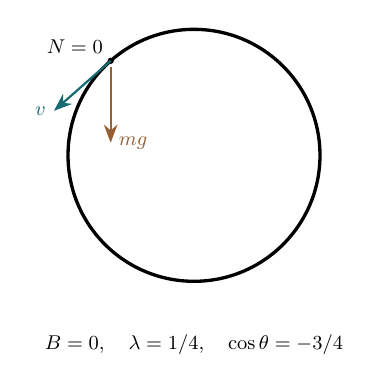
\begin{tikzpicture}[scale=.8,transform shape]
\draw[very thick] (0,0) circle (2);\fill (-1.322875656,1.5) circle(.05) node[above left] {$N=0$};\draw[motion] (-1.322875656,1.5)--(-2.222875656,.706274607) node[left] {$v$};\draw[force] (-1.322875656,1.4)--(-1.322875656,.2) node[right] {$mg$};\node at (0,-3) {$B=0,\quad\lambda=1/4,\quad\cos\theta=-3/4$};
\end{tikzpicture}
\figcaption{变图电试2.3V2\quad 无磁场时在上半环达到接触终点并沿切向离开}
\end{minipage}\end{center}

\Needspace{20\baselineskip}
\item 磁场反向而最高点初速度方向不变，说明最低点的受力条件。
\textbf{解：}变图电试2.3V3中反向磁场使洛伦兹力沿径向向外。最低点速度仍由能量给$v_b^2=(\lambda+4)Rg$，方向向右；磁力、重力和外侧支持力此时都向下。向心方向向上，径向方程给$N_b=-QBv_b-mg-mv_b^2/R<0$。单侧圆环提供向外推力，因而无法实现这一最低点所需的径向作用，反向磁场和原绕行方向组合不能维持全环外侧接触。
\begin{center}\begin{minipage}{.98\linewidth}\centering
\begin{tikzpicture}[scale=.8,transform shape]
\draw[very thick] (0,0) circle (2);\fill (0,-2) circle(.05) node[above right] {$B_{\rm p}$};\draw[motion] (0,-2)--(1.4,-2) node[right] {$v_b$};\draw[force] (-.25,-2)--(-.25,-3.3) node[below] {$QBv_b$};\draw[force] (.25,-2)--(.25,-3) node[right] {$mg$};\node at (0,3) {$\boldsymbol B$反向：$\odot$};
\end{tikzpicture}
\figcaption{变图电试2.3V3\quad 反向磁场使最低点的磁力和重力都指向环外}
\end{minipage}\end{center}

\Needspace{20\baselineskip}
\item 给定$\lambda>0$，求全环严格正支持力的磁场条件，并说明阈值随初速的变化。
\textbf{解：}变图电试2.3V4由$\mu>(\lambda+5)^2/(\lambda+4)$和$\mu=Q^2B^2R/(m^2g)$，得$B>(m/Q)\sqrt{g/R}(\lambda+5)/\sqrt{\lambda+4}$。允许最低点零支持力时可取等号。无量纲阈值$b(\lambda)=(\lambda+5)/\sqrt{\lambda+4}$的导数为$(\lambda+3)/[2(\lambda+4)^{3/2}]>0$，所以初速增大时要求的磁场也增大；$\lambda\to0^+$时阈值趋于$5/2$。
\begin{center}\begin{minipage}{.98\linewidth}\centering
\begin{tikzpicture}[scale=.8,transform shape]
\draw[axis] (0,0)--(10.7,0) node[right] {$\lambda$};
\draw[axis] (0,0)--(0,3.2) node[above] {$QB_{\rm crit}\sqrt{R/g}/m$};\foreach \y/\lab in {0/2.4,1.44/3,2.64/3.5}{\draw[thin] (0,\y)--(-.08,\y) node[left] {$\lab$};}
\node[above] at (5,3.5) {非零初速增大时临界场强增加};
\draw[traj] plot coordinates {(0.000000000,0.240000000) (0.083333333,0.262476419) (0.166666667,0.284905131) (0.250000000,0.307285374) (0.333333333,0.329616455) (0.416666667,0.351897751) (0.500000000,0.374128698) (0.583333333,0.396308791) (0.666666667,0.418437578) (0.750000000,0.440514658) (0.833333333,0.462539674) (0.916666667,0.484512316) (1.000000000,0.506432311) (1.083333333,0.528299427) (1.166666667,0.550113463) (1.250000000,0.571874255) (1.333333333,0.593581667) (1.416666667,0.615235593) (1.500000000,0.636835953) (1.583333333,0.658382691) (1.666666667,0.679875775) (1.750000000,0.701315196) (1.833333333,0.722700962) (1.916666667,0.744033103) (2.000000000,0.765311664) (2.083333333,0.786536707) (2.166666667,0.807708311) (2.250000000,0.828826566) (2.333333333,0.849891578) (2.416666667,0.870903463) (2.500000000,0.891862350) (2.583333333,0.912768379) (2.666666667,0.933621697) (2.750000000,0.954422464) (2.833333333,0.975170845) (2.916666667,0.995867015) (3.000000000,1.016511156) (3.083333333,1.037103455) (3.166666667,1.057644108) (3.250000000,1.078133315) (3.333333333,1.098571280) (3.416666667,1.118958214) (3.500000000,1.139294333) (3.583333333,1.159579855) (3.666666667,1.179815002) (3.750000000,1.200000000) (3.833333333,1.220135079) (3.916666667,1.240220469) (4.000000000,1.260256406) (4.083333333,1.280243125) (4.166666667,1.300180865) (4.250000000,1.320069866) (4.333333333,1.339910371) (4.416666667,1.359702621) (4.500000000,1.379446862) (4.583333333,1.399143338) (4.666666667,1.418792296) (4.750000000,1.438393981) (4.833333333,1.457948643) (4.916666667,1.477456527) (5.000000000,1.496917882) (5.083333333,1.516332955) (5.166666667,1.535701995) (5.250000000,1.555025250) (5.333333333,1.574302966) (5.416666667,1.593535392) (5.500000000,1.612722774) (5.583333333,1.631865358) (5.666666667,1.650963391) (5.750000000,1.670017117) (5.833333333,1.689026782) (5.916666667,1.707992629) (6.000000000,1.726914901) (6.083333333,1.745793841) (6.166666667,1.764629688) (6.250000000,1.783422685) (6.333333333,1.802173070) (6.416666667,1.820881081) (6.500000000,1.839546955) (6.583333333,1.858170929) (6.666666667,1.876753237) (6.750000000,1.895294113) (6.833333333,1.913793789) (6.916666667,1.932252496) (7.000000000,1.950670465) (7.083333333,1.969047924) (7.166666667,1.987385101) (7.250000000,2.005682221) (7.333333333,2.023939509) (7.416666667,2.042157189) (7.500000000,2.060335482) (7.583333333,2.078474610) (7.666666667,2.096574791) (7.750000000,2.114636243) (7.833333333,2.132659182) (7.916666667,2.150643824) (8.000000000,2.168590383) (8.083333333,2.186499069) (8.166666667,2.204370095) (8.250000000,2.222203669) (8.333333333,2.240000000) (8.416666667,2.257759293) (8.500000000,2.275481755) (8.583333333,2.293167588) (8.666666667,2.310816994) (8.750000000,2.328430175) (8.833333333,2.346007330) (8.916666667,2.363548657) (9.000000000,2.381054352) (9.083333333,2.398524610) (9.166666667,2.415959625) (9.250000000,2.433359589) (9.333333333,2.450724694) (9.416666667,2.468055128) (9.500000000,2.485351080) (9.583333333,2.502612736) (9.666666667,2.519840282) (9.750000000,2.537033902) (9.833333333,2.554193778) (9.916666667,2.571320092) (10.000000000,2.588413023)};
\node[below] at (0,-.12) {$0$极限};
\node[below] at (5,-.12) {$3$};
\node[below] at (10,-.12) {$6$};
\end{tikzpicture}
\figcaption{变图电试2.3V4\quad 非零初速增大时临界场强增加}
\end{minipage}\end{center}

\Needspace{20\baselineskip}
\item 固定磁场参数$\mu$，求能够持续外侧绕行的全部初速参数$\lambda>0$。
\textbf{解：}变图电试2.3V5将保持接触条件写成$\lambda^2+(10-\mu)\lambda+25-4\mu\le0$。阈值函数对$\lambda>0$严格递增，起始极限为$25/4$，因此存在非零允许初速的条件是$\mu>25/4$。此时正根$\lambda_{\max}=[\mu-10+\sqrt{\mu(\mu-4)}]/2$，另一根为负，所以$0<\lambda\le\lambda_{\max}$。若要求处处$N>0$，上限改为严格小于，等号对应最低点的孤立零支持力。
\begin{center}\begin{minipage}{.98\linewidth}\centering
\begin{tikzpicture}[scale=.8,transform shape]
\draw[axis] (0,0)--(10.7,0) node[right] {$\mu$};
\draw[axis] (0,0)--(0,3.2) node[above] {$\lambda_{\max}$};\foreach \y/\lab in {0/0,1.2/4,2.4/8}{\draw[thin] (0,\y)--(-.08,\y) node[left] {$\lab$};}
\node[above] at (5,3.5) {固定磁场允许的初速参数上限};
\draw[traj] plot coordinates {(0.000000000,0.000000000) (0.083333333,0.023303738) (0.166666667,0.046550775) (0.250000000,0.069744604) (0.333333333,0.092888425) (0.416666667,0.115985172) (0.500000000,0.139037546) (0.583333333,0.162048035) (0.666666667,0.185018939) (0.750000000,0.207952384) (0.833333333,0.230850340) (0.916666667,0.253714638) (1.000000000,0.276546978) (1.083333333,0.299348947) (1.166666667,0.322122020) (1.250000000,0.344867580) (1.333333333,0.367586916) (1.416666667,0.390281237) (1.500000000,0.412951676) (1.583333333,0.435599298) (1.666666667,0.458225101) (1.750000000,0.480830026) (1.833333333,0.503414959) (1.916666667,0.525980733) (2.000000000,0.548528137) (2.083333333,0.571057915) (2.166666667,0.593570770) (2.250000000,0.616067367) (2.333333333,0.638548336) (2.416666667,0.661014275) (2.500000000,0.683465749) (2.583333333,0.705903297) (2.666666667,0.728327428) (2.750000000,0.750738630) (2.833333333,0.773137362) (2.916666667,0.795524066) (3.000000000,0.817899159) (3.083333333,0.840263041) (3.166666667,0.862616092) (3.250000000,0.884958677) (3.333333333,0.907291141) (3.416666667,0.929613817) (3.500000000,0.951927020) (3.583333333,0.974231055) (3.666666667,0.996526212) (3.750000000,1.018812767) (3.833333333,1.041090988) (3.916666667,1.063361129) (4.000000000,1.085623435) (4.083333333,1.107878140) (4.166666667,1.130125470) (4.250000000,1.152365642) (4.333333333,1.174598862) (4.416666667,1.196825330) (4.500000000,1.219045239) (4.583333333,1.241258773) (4.666666667,1.263466110) (4.750000000,1.285667421) (4.833333333,1.307862870) (4.916666667,1.330052617) (5.000000000,1.352236815) (5.083333333,1.374415610) (5.166666667,1.396589145) (5.250000000,1.418757557) (5.333333333,1.440920980) (5.416666667,1.463079539) (5.500000000,1.485233360) (5.583333333,1.507382561) (5.666666667,1.529527257) (5.750000000,1.551667561) (5.833333333,1.573803579) (5.916666667,1.595935415) (6.000000000,1.618063172) (6.083333333,1.640186945) (6.166666667,1.662306830) (6.250000000,1.684422918) (6.333333333,1.706535298) (6.416666667,1.728644055) (6.500000000,1.750749272) (6.583333333,1.772851031) (6.666666667,1.794949409) (6.750000000,1.817044482) (6.833333333,1.839136323) (6.916666667,1.861225005) (7.000000000,1.883310596) (7.083333333,1.905393163) (7.166666667,1.927472771) (7.250000000,1.949549485) (7.333333333,1.971623365) (7.416666667,1.993694471) (7.500000000,2.015762862) (7.583333333,2.037828593) (7.666666667,2.059891721) (7.750000000,2.081952298) (7.833333333,2.104010376) (7.916666667,2.126066006) (8.000000000,2.148119237) (8.083333333,2.170170117) (8.166666667,2.192218692) (8.250000000,2.214265007) (8.333333333,2.236309108) (8.416666667,2.258351037) (8.500000000,2.280390835) (8.583333333,2.302428544) (8.666666667,2.324464204) (8.750000000,2.346497852) (8.833333333,2.368529528) (8.916666667,2.390559267) (9.000000000,2.412587106) (9.083333333,2.434613080) (9.166666667,2.456637222) (9.250000000,2.478659567) (9.333333333,2.500680146) (9.416666667,2.522698992) (9.500000000,2.544716136) (9.583333333,2.566731607) (9.666666667,2.588745435) (9.750000000,2.610757649) (9.833333333,2.632768278) (9.916666667,2.654777348) (10.000000000,2.676784887)};
\node[below] at (0,-.12) {$25/4$};
\node[below] at (4.285714285714286,-.12) {$10$};
\node[below] at (10,-.12) {$15$};
\end{tikzpicture}
\figcaption{变图电试2.3V5\quad 固定磁场允许的初速参数上限}
\end{minipage}\end{center}

\Needspace{20\baselineskip}
\item 在保持全环接触时求绕行一周的时间，并讨论极小初速。
\textbf{解：}变图电试2.3V6由$|\dot\theta|=\sqrt{g/R}\sqrt{\lambda+2+2\cos\theta}$，整周时间$P=\sqrt{R/g}\int_{-\pi}^{\pi}[\lambda+2+2\cos\theta]^{-1/2}\mathrm d\theta$。令半角变量，得到$P=4\sqrt{R/g}\,K(4/(\lambda+4))/\sqrt{\lambda+4}$，这里$K(m)=\int_0^{\pi/2}(1-m\sin^2u)^{-1/2}\mathrm du$。$\lambda\to0^+$时$P\sim2\sqrt{R/g}\ln(8/\sqrt\lambda)$，趋于无穷。任意非零初速都能在临界场下绕行，初速趋零时在最高点附近停留的时间增长。
\begin{center}\begin{minipage}{.98\linewidth}\centering
\begin{tikzpicture}[scale=.8,transform shape]
\draw[axis] (0,0)--(10.7,0) node[right] {$\lambda$};
\draw[axis] (0,0)--(0,3.2) node[above] {$P\sqrt{g/R}$};\foreach \y/\lab in {0/0,1.4/4,2.8/8}{\draw[thin] (0,\y)--(-.08,\y) node[left] {$\lab$};}
\node[above] at (5,3.5) {小初速增加最高点附近的停留时间};
\draw[traj] plot coordinates {(0.060000000,2.679201085) (0.142833333,2.371910909) (0.225666667,2.208694422) (0.308500000,2.096494365) (0.391333333,2.010750384) (0.474166667,1.941261397) (0.557000000,1.882794907) (0.639833333,1.832305029) (0.722666667,1.787860907) (0.805500000,1.748160652) (0.888333333,1.712284388) (0.971166667,1.679557800) (1.054000000,1.649471666) (1.136833333,1.621631902) (1.219666667,1.595727185) (1.302500000,1.571507229) (1.385333333,1.548767755) (1.468166667,1.527339829) (1.551000000,1.507082123) (1.633833333,1.487875185) (1.716666667,1.469617130) (1.799500000,1.452220338) (1.882333333,1.435608899) (1.965166667,1.419716607) (2.048000000,1.404485362) (2.130833333,1.389863893) (2.213666667,1.375806724) (2.296500000,1.362273325) (2.379333333,1.349227418) (2.462166667,1.336636397) (2.545000000,1.324470847) (2.627833333,1.312704137) (2.710666667,1.301312078) (2.793500000,1.290272632) (2.876333333,1.279565661) (2.959166667,1.269172716) (3.042000000,1.259076849) (3.124833333,1.249262455) (3.207666667,1.239715132) (3.290500000,1.230421561) (3.373333333,1.221369399) (3.456166667,1.212547184) (3.539000000,1.203944253) (3.621833333,1.195550671) (3.704666667,1.187357163) (3.787500000,1.179355058) (3.870333333,1.171536235) (3.953166667,1.163893083) (4.036000000,1.156418452) (4.118833333,1.149105619) (4.201666667,1.141948257) (4.284500000,1.134940400) (4.367333333,1.128076419) (4.450166667,1.121350995) (4.533000000,1.114759099) (4.615833333,1.108295968) (4.698666667,1.101957088) (4.781500000,1.095738178) (4.864333333,1.089635173) (4.947166667,1.083644209) (5.030000000,1.077761610) (5.112833333,1.071983878) (5.195666667,1.066307680) (5.278500000,1.060729837) (5.361333333,1.055247316) (5.444166667,1.049857221) (5.527000000,1.044556784) (5.609833333,1.039343358) (5.692666667,1.034214412) (5.775500000,1.029167519) (5.858333333,1.024200357) (5.941166667,1.019310699) (6.024000000,1.014496407) (6.106833333,1.009755431) (6.189666667,1.005085800) (6.272500000,1.000485624) (6.355333333,0.995953082) (6.438166667,0.991486424) (6.521000000,0.987083967) (6.603833333,0.982744088) (6.686666667,0.978465227) (6.769500000,0.974245876) (6.852333333,0.970084587) (6.935166667,0.965979957) (7.018000000,0.961930637) (7.100833333,0.957935322) (7.183666667,0.953992753) (7.266500000,0.950101713) (7.349333333,0.946261026) (7.432166667,0.942469554) (7.515000000,0.938726197) (7.597833333,0.935029891) (7.680666667,0.931379606) (7.763500000,0.927774343) (7.846333333,0.924213137) (7.929166667,0.920695051) (8.012000000,0.917219178) (8.094833333,0.913784637) (8.177666667,0.910390575) (8.260500000,0.907036164) (8.343333333,0.903720601) (8.426166667,0.900443105) (8.509000000,0.897202920) (8.591833333,0.893999309) (8.674666667,0.890831557) (8.757500000,0.887698971) (8.840333333,0.884600875) (8.923166667,0.881536612) (9.006000000,0.878505545) (9.088833333,0.875507051) (9.171666667,0.872540527) (9.254500000,0.869605384) (9.337333333,0.866701050) (9.420166667,0.863826966) (9.503000000,0.860982591) (9.585833333,0.858167394) (9.668666667,0.855380860) (9.751500000,0.852622488) (9.834333333,0.849891786) (9.917166667,0.847188278) (10.000000000,0.844511498)};
\node[below] at (0,-.12) {$0$};
\node[below] at (5,-.12) {$2.5$};
\node[below] at (10,-.12) {$5$};
\end{tikzpicture}
\figcaption{变图电试2.3V6\quad 小初速增加最高点附近的停留时间}
\end{minipage}\end{center}

\Needspace{20\baselineskip}
\item 给定$\lambda,\mu$，求沿环支持力最大的位置与最大值。
\textbf{解：}变图电试2.3V7由$n'(c)=\sqrt\mu/\sqrt{\lambda+2+2c}-3$。若$\mu\le9\lambda$，函数全程递减，最大值在最高点；若$\mu\ge9(\lambda+4)$，函数全程递增，最大值在最低点。中间范围$9\lambda<\mu<9(\lambda+4)$存在唯一最大点$c_*=[\mu/9-\lambda-2]/2$，代入得$n_{\max}=\mu/6+(\lambda+2)/2$。该点的速率满足$v_*^2/(Rg)=\mu/9$，位于左右两侧同一高度的两个位置。
\begin{center}\begin{minipage}{.98\linewidth}\centering
\begin{tikzpicture}[scale=.8,transform shape]
\draw[axis] (0,0)--(10.7,0) node[right] {$\mu$};
\draw[axis] (0,0)--(0,3.2) node[above] {$N_{\max}/(mg)$};\foreach \y/\lab in {0/0,1.4/5,2.8/10}{\draw[thin] (0,\y)--(-.08,\y) node[left] {$\lab$};}
\node[above] at (5,3.5) {$\lambda=1$时最大支持力及其位置随磁场变化};
\draw[traj] plot coordinates {(0.000000000,0.751318840) (0.083333333,0.769702973) (0.166666667,0.787658132) (0.250000000,0.805213015) (0.333333333,0.822393255) (0.416666667,0.839221862) (0.500000000,0.855866667) (0.583333333,0.872511111) (0.666666667,0.889155556) (0.750000000,0.905800000) (0.833333333,0.922444444) (0.916666667,0.939088889) (1.000000000,0.955733333) (1.083333333,0.972377778) (1.166666667,0.989022222) (1.250000000,1.005666667) (1.333333333,1.022311111) (1.416666667,1.038955556) (1.500000000,1.055600000) (1.583333333,1.072244444) (1.666666667,1.088888889) (1.750000000,1.105533333) (1.833333333,1.122177778) (1.916666667,1.138822222) (2.000000000,1.155466667) (2.083333333,1.172111111) (2.166666667,1.188755556) (2.250000000,1.205400000) (2.333333333,1.222044444) (2.416666667,1.238688889) (2.500000000,1.255333333) (2.583333333,1.271977778) (2.666666667,1.288622222) (2.750000000,1.305266667) (2.833333333,1.321911111) (2.916666667,1.338555556) (3.000000000,1.355200000) (3.083333333,1.371844444) (3.166666667,1.388488889) (3.250000000,1.405133333) (3.333333333,1.421777778) (3.416666667,1.438422222) (3.500000000,1.455066667) (3.583333333,1.471711111) (3.666666667,1.488355556) (3.750000000,1.505000000) (3.833333333,1.521644444) (3.916666667,1.538288889) (4.000000000,1.554933333) (4.083333333,1.571577778) (4.166666667,1.588222222) (4.250000000,1.604866667) (4.333333333,1.621511111) (4.416666667,1.638155556) (4.500000000,1.654800000) (4.583333333,1.671444444) (4.666666667,1.688088889) (4.750000000,1.704733333) (4.833333333,1.721377778) (4.916666667,1.738022222) (5.000000000,1.754666667) (5.083333333,1.771311111) (5.166666667,1.787955556) (5.250000000,1.804600000) (5.333333333,1.821244444) (5.416666667,1.837888889) (5.500000000,1.854533333) (5.583333333,1.871177778) (5.666666667,1.887822222) (5.750000000,1.904466667) (5.833333333,1.921111111) (5.916666667,1.937755556) (6.000000000,1.954400000) (6.083333333,1.971044444) (6.166666667,1.987688889) (6.250000000,2.004333333) (6.333333333,2.020977778) (6.416666667,2.037622222) (6.500000000,2.054266667) (6.583333333,2.070911111) (6.666666667,2.087555556) (6.750000000,2.104200000) (6.833333333,2.120844444) (6.916666667,2.137488889) (7.000000000,2.154133333) (7.083333333,2.170777778) (7.166666667,2.187422222) (7.250000000,2.204066667) (7.333333333,2.220711111) (7.416666667,2.237355556) (7.500000000,2.254000000) (7.583333333,2.270644444) (7.666666667,2.287288889) (7.750000000,2.303933333) (7.833333333,2.320577778) (7.916666667,2.337222222) (8.000000000,2.353866667) (8.083333333,2.370511111) (8.166666667,2.387155556) (8.250000000,2.403800000) (8.333333333,2.420444444) (8.416666667,2.437088889) (8.500000000,2.453733333) (8.583333333,2.470377778) (8.666666667,2.487022222) (8.750000000,2.503666667) (8.833333333,2.520311100) (8.916666667,2.536921468) (9.000000000,2.553466665) (9.083333333,2.569947451) (9.166666667,2.586364573) (9.250000000,2.602718763) (9.333333333,2.619010739) (9.416666667,2.635241206) (9.500000000,2.651410856) (9.583333333,2.667520366) (9.666666667,2.683570404) (9.750000000,2.699561622) (9.833333333,2.715494663) (9.916666667,2.731370158) (10.000000000,2.747188724)};
\node[below] at (0,-.12) {$36/5$};
\node[below] at (0.42056074766355145,-.12) {$9$};
\node[below] at (8.83177570093458,-.12) {$45$};
\end{tikzpicture}
\figcaption{变图电试2.3V7\quad $\lambda=1$时最大支持力及其位置随磁场变化}
\end{minipage}\end{center}

\Needspace{20\baselineskip}
\item 随着磁场增大，全环最小支持力总出现在最低点吗？求两个端点支持力相等的场参数。
\textbf{解：}变图电试2.3V8利用凹性，最小值为$n(-1)$与$n(1)$中的较小者。两者之差为$n(-1)-n(1)=6-\sqrt\mu(\sqrt{\lambda+4}-\sqrt\lambda)$，故相等时$\mu_s=36/(\sqrt{\lambda+4}-\sqrt\lambda)^2$。低于$\mu_s$时最低点支持力较小，高于它时最高点支持力较小。对$\lambda=1$，$\mu_s=(9/4)(\sqrt5+1)^2$；图中两端曲线在此相交。接触阈值由最先降为零的端点决定，强磁场下最小支持力的位置可随场强改变。
\begin{center}\begin{minipage}{.98\linewidth}\centering
\begin{tikzpicture}[scale=.8,transform shape]
\draw[axis] (0,0)--(10.7,0) node[right] {$\mu$};
\draw[axis] (0,0)--(0,3.2) node[above] {$N_A/(mg),\ N_b/(mg)$};\foreach \y/\lab in {0/0,1.6/4,2.8/7}{\draw[thin] (0,\y)--(-.08,\y) node[left] {$\lab$};}
\node[above] at (5,3.5) {$\lambda=1$：实线最高点，虚线最低点};
\draw[traj] plot coordinates {(0.000000000,1.073312629) (0.083333333,1.090443335) (0.166666667,1.107309051) (0.250000000,1.123921705) (0.333333333,1.140292360) (0.416666667,1.156431292) (0.500000000,1.172348071) (0.583333333,1.188051626) (0.666666667,1.203550304) (0.750000000,1.218851919) (0.833333333,1.233963803) (0.916666667,1.248892843) (1.000000000,1.263645520) (1.083333333,1.278227940) (1.166666667,1.292645865) (1.250000000,1.306904740) (1.333333333,1.321009715) (1.416666667,1.334965667) (1.500000000,1.348777224) (1.583333333,1.362448776) (1.666666667,1.375984496) (1.750000000,1.389388355) (1.833333333,1.402664132) (1.916666667,1.415815431) (2.000000000,1.428845688) (2.083333333,1.441758186) (2.166666667,1.454556061) (2.250000000,1.467242311) (2.333333333,1.479819809) (2.416666667,1.492291303) (2.500000000,1.504659430) (2.583333333,1.516926718) (2.666666667,1.529095593) (2.750000000,1.541168388) (2.833333333,1.553147342) (2.916666667,1.565034611) (3.000000000,1.576832268) (3.083333333,1.588542309) (3.166666667,1.600166658) (3.250000000,1.611707169) (3.333333333,1.623165631) (3.416666667,1.634543769) (3.500000000,1.645843249) (3.583333333,1.657065680) (3.666666667,1.668212616) (3.750000000,1.679285562) (3.833333333,1.690285972) (3.916666667,1.701215252) (4.000000000,1.712074765) (4.083333333,1.722865830) (4.166666667,1.733589725) (4.250000000,1.744247689) (4.333333333,1.754840923) (4.416666667,1.765370594) (4.500000000,1.775837830) (4.583333333,1.786243731) (4.666666667,1.796589361) (4.750000000,1.806875757) (4.833333333,1.817103923) (4.916666667,1.827274838) (5.000000000,1.837389452) (5.083333333,1.847448691) (5.166666667,1.857453454) (5.250000000,1.867404616) (5.333333333,1.877303030) (5.416666667,1.887149526) (5.500000000,1.896944912) (5.583333333,1.906689977) (5.666666667,1.916385487) (5.750000000,1.926032191) (5.833333333,1.935630819) (5.916666667,1.945182082) (6.000000000,1.954686676) (6.083333333,1.964145276) (6.166666667,1.973558546) (6.250000000,1.982927129) (6.333333333,1.992251657) (6.416666667,2.001532746) (6.500000000,2.010770996) (6.583333333,2.019966996) (6.666666667,2.029121321) (6.750000000,2.038234530) (6.833333333,2.047307174) (6.916666667,2.056339790) (7.000000000,2.065332903) (7.083333333,2.074287026) (7.166666667,2.083202663) (7.250000000,2.092080304) (7.333333333,2.100920433) (7.416666667,2.109723521) (7.500000000,2.118490028) (7.583333333,2.127220409) (7.666666667,2.135915104) (7.750000000,2.144574550) (7.833333333,2.153199170) (7.916666667,2.161789382) (8.000000000,2.170345595) (8.083333333,2.178868208) (8.166666667,2.187357614) (8.250000000,2.195814200) (8.333333333,2.204238342) (8.416666667,2.212630410) (8.500000000,2.220990770) (8.583333333,2.229319777) (8.666666667,2.237617781) (8.750000000,2.245885126) (8.833333333,2.254122150) (8.916666667,2.262329183) (9.000000000,2.270506551) (9.083333333,2.278654574) (9.166666667,2.286773564) (9.250000000,2.294863830) (9.333333333,2.302925675) (9.416666667,2.310959397) (9.500000000,2.318965287) (9.583333333,2.326943632) (9.666666667,2.334894716) (9.750000000,2.342818815) (9.833333333,2.350716203) (9.916666667,2.358587148) (10.000000000,2.366431913)};
\draw[dashed,thick,color=warm] plot coordinates {(0.000000000,0.000000000) (0.083333333,0.038305422) (0.166666667,0.076018309) (0.250000000,0.113165335) (0.333333333,0.149771232) (0.416666667,0.185858980) (0.500000000,0.221449980) (0.583333333,0.256564197) (0.666666667,0.291220293) (0.750000000,0.325435745) (0.833333333,0.359226945) (0.916666667,0.392609294) (1.000000000,0.425597282) (1.083333333,0.458204565) (1.166666667,0.490444026) (1.250000000,0.522327839) (1.333333333,0.553867521) (1.416666667,0.585073980) (1.500000000,0.615957559) (1.583333333,0.646528079) (1.666666667,0.676794869) (1.750000000,0.706766808) (1.833333333,0.736452348) (1.916666667,0.765859546) (2.000000000,0.794996088) (2.083333333,0.823869311) (2.166666667,0.852486229) (2.250000000,0.880853547) (2.333333333,0.908977687) (2.416666667,0.936864796) (2.500000000,0.964520768) (2.583333333,0.991951258) (2.666666667,1.019161691) (2.750000000,1.046157280) (2.833333333,1.072943036) (2.916666667,1.099523777) (3.000000000,1.125904139) (3.083333333,1.152088587) (3.166666667,1.178081423) (3.250000000,1.203886791) (3.333333333,1.229508690) (3.416666667,1.254950980) (3.500000000,1.280217385) (3.583333333,1.305311503) (3.666666667,1.330236811) (3.750000000,1.354996671) (3.833333333,1.379594334) (3.916666667,1.404032948) (4.000000000,1.428315556) (4.083333333,1.452445111) (4.166666667,1.476424469) (4.250000000,1.500256402) (4.333333333,1.523943595) (4.416666667,1.547488653) (4.500000000,1.570894106) (4.583333333,1.594162407) (4.666666667,1.617295940) (4.750000000,1.640297019) (4.833333333,1.663167894) (4.916666667,1.685910751) (5.000000000,1.708527717) (5.083333333,1.731020858) (5.166666667,1.753392188) (5.250000000,1.775643663) (5.333333333,1.797777190) (5.416666667,1.819794624) (5.500000000,1.841697773) (5.583333333,1.863488400) (5.666666667,1.885168219) (5.750000000,1.906738905) (5.833333333,1.928202090) (5.916666667,1.949559365) (6.000000000,1.970812281) (6.083333333,1.991962356) (6.166666667,2.013011066) (6.250000000,2.033959855) (6.333333333,2.054810134) (6.416666667,2.075563279) (6.500000000,2.096220635) (6.583333333,2.116783516) (6.666666667,2.137253207) (6.750000000,2.157630964) (6.833333333,2.177918013) (6.916666667,2.198115556) (7.000000000,2.218224767) (7.083333333,2.238246795) (7.166666667,2.258182764) (7.250000000,2.278033775) (7.333333333,2.297800904) (7.416666667,2.317485206) (7.500000000,2.337087713) (7.583333333,2.356609437) (7.666666667,2.376051368) (7.750000000,2.395414476) (7.833333333,2.414699714) (7.916666667,2.433908012) (8.000000000,2.453040284) (8.083333333,2.472097427) (8.166666667,2.491080317) (8.250000000,2.509989817) (8.333333333,2.528826770) (8.416666667,2.547592007) (8.500000000,2.566286339) (8.583333333,2.584910564) (8.666666667,2.603465466) (8.750000000,2.621951812) (8.833333333,2.640370357) (8.916666667,2.658721841) (9.000000000,2.677006992) (9.083333333,2.695226524) (9.166666667,2.713381138) (9.250000000,2.731471524) (9.333333333,2.749498357) (9.416666667,2.767462304) (9.500000000,2.785364018) (9.583333333,2.803204141) (9.666666667,2.820983305) (9.750000000,2.838702129) (9.833333333,2.856361226) (9.916666667,2.873961193) (10.000000000,2.891502622)};
\node[below] at (0,-.12) {$36/5$};
\node[below] at (5.885721546312609,-.12) {$\mu_s$};
\node[below] at (10,-.12) {$35$};
\end{tikzpicture}
\figcaption{变图电试2.3V8\quad $\lambda=1$：实线最高点，虚线最低点}
\end{minipage}\end{center}
\end{enumerate}

\Needspace{13\baselineskip}

\pdfbookmark[2]{第 4 题 匀强磁场中电阻网络的总安培力}{q4}

\section*{第 4 题\quad 匀强磁场中电阻网络的总安培力}\label{q:4}


平面$\Sigma_1$与$\Sigma_2$相交于直线$MN$，夹角$\phi=45^\circ$。匀强磁场$\boldsymbol B$平行于$\Sigma_1$、垂直$MN$。
$\Sigma_2$内有长方形网络$abcdef$：$a,b$为左下、左上角，$d,e$为右上、右下角，$c,f$分别是上下长边中点。七段$ab,bc,cd,de,ef,fa,fc$均长$l$，且$ab\parallel MN$。各电阻为
\[
R_{ab}=R_{fc}=R_{ed}=R,\quad
R_{af}=R_{bc}=2R,\quad R_{fe}=R_{cd}=4R.
\]
总电流$I$从$a$流入、从$d$流出。求网络所受总磁场力大小，并说明是否需要先求七段电流。
取$\hat e_u$由$a$指向$f$，$\hat e_v$由$a$指向$b$，$\hat n=\hat e_u\times\hat e_v$，选择磁场为
$\boldsymbol B=B(\cos\phi\,\hat e_u+\sin\phi\,\hat n)$。


\begin{center}\begin{minipage}{.98\linewidth}\centering
\begin{tikzpicture}[scale=.7,transform shape]

\coordinate (a) at (0,0);\coordinate (b) at (0,2);
\coordinate (c) at (2,2);\coordinate (d) at (4,2);
\coordinate (e) at (4,0);\coordinate (f) at (2,0);
\foreach \p/\q/\lab in {a/b/R,b/c/2R,c/d/4R,d/e/R,e/f/4R,f/a/2R,f/c/R}{
\draw[object] (\p)--(\q) node[midway,fill=white,inner sep=2pt] {$\lab$};}
\foreach \p in {a,b,c,d,e,f}{\fill (\p) circle (1.6pt);}
\node[below left] at (a) {$a$};\node[above left] at (b) {$b$};
\node[above] at (c) {$c$};\node[above right] at (d) {$d$};
\node[below right] at (e) {$e$};\node[below] at (f) {$f$};
\draw[motion] (-1,0)--(-.15,0) node[midway,above] {$I$};
\draw[motion] (4.15,2)--(5,2) node[midway,above] {$I$};
\draw[axis] (-.7,-.7)--(1,-.7) node[right] {$\hat e_u$};
\draw[axis] (-.7,-.7)--(-.7,1) node[left] {$\hat e_v\parallel MN$};

\begin{scope}[xshift=8cm,yshift=.3cm]
\draw[axis] (0,0)--(2.7,0) node[right] {$\Sigma_2,\hat e_u$};
\draw[axis] (0,0)--(0,2.6) node[above] {$\hat n$};
\draw[motion] (0,0)--(1.8,1.8) node[right] {$\boldsymbol B$};
\draw[guide] (-.5,-.5)--(2.1,2.1) node[above] {$\Sigma_1$};
\draw[axis] (.7,0) arc[start angle=0,end angle=45,radius=.7];
\node at (1,.42) {$\phi$};
\node[align=center] at (1.2,-1) {沿$MN$观察\\截面};
\end{scope}

\end{tikzpicture}
\figcaption{图电试2.4\quad 网络长边为两段l；右侧截面给磁场与网络面的夹角。}
\end{minipage}\end{center}

\Needspace{8\baselineskip}

\pdfbookmark[3]{题型定位}{q4-h0}

\subsection*{题型定位}

把匀强磁场中的开放电流网络按输入、输出端点等效，再计算端点位移与磁场的空间叉积。支路电流由电阻网络决定，但它们的位移加权和由结点守恒固定。给定电阻数据的计算作为具体电流分布说明，保留数值解与端点结果的联系。

\Needspace{8\baselineskip}

\pdfbookmark[3]{知识点}{q4-h1}

\subsection*{知识点}

每个直线支路的安培力为$I\boldsymbol L\times\boldsymbol B$，磁场均匀时可先对$I\boldsymbol L$求和。内部结点的流入、流出电流相等，使对应位置矢量的系数相消。闭合回路的合力为零，磁力矩由磁矩与磁场确定。空间投影把端点距离分成沿场与垂直场两部分，实际有效长度为后者。

\Needspace{8\baselineskip}

\pdfbookmark[3]{物理图像}{q4-h2}

\subsection*{物理图像}

题图给出七段电阻、两个端点和磁场相对网络面的方向。解图电试2.4A把开放路径与右侧闭合环叠加，图B把对角线沿磁场分解。图C将给定电阻对应的七个带方向支路电流标在同一平面网络中，每个结点的电流流入与流出相等。端点$a,d$的位置差决定合力，内部路径和环流仍影响局部受力与力矩。

\Needspace{8\baselineskip}

\pdfbookmark[3]{解题入口}{q4-h3}

\subsection*{解题入口}

从一个支路写$I_{ij}(\boldsymbol r_j-\boldsymbol r_i)\times\boldsymbol B$，把所有支路按结点位置矢量归并。输入点留下$-I\boldsymbol r_a$、输出点留下$+I\boldsymbol r_d$，内部结点相消。再用$\hat e_u,\hat e_v,\hat n$组成的右手基逐项叉乘，或从端点位移中减去沿磁场投影，得到相同合力大小。

\Needspace{8\baselineskip}

\pdfbookmark[3]{标准解法}{q4-h4}

\subsection*{标准解法}


图电试2.4中各段电流大小会随电阻改变，但任一内部结点都满足电流守恒。先以任意有向线段$i\to j$表示一个支路，电流代数值为$I_{ij}$。匀强场中该段磁场力为
\[
\boldsymbol F_{ij}
=I_{ij}(\boldsymbol r_j-\boldsymbol r_i)\times\boldsymbol B.
\]
匀强磁场在每个支路上取同一个矢量，所以先把电流乘位移求和，再与$\boldsymbol B$作叉积。对结点$k$，每条流入支路给$+I\boldsymbol r_k$，每条流出支路给$-I\boldsymbol r_k$。把网络全部支路相加。每个内部结点的$\boldsymbol r_k$系数等于流入电流减流出电流，因结点守恒而为零；只剩输入、输出结点：
\[
\sum I_{ij}(\boldsymbol r_j-\boldsymbol r_i)
=I(\boldsymbol r_d-\boldsymbol r_a).
\]
\begin{center}\begin{minipage}{.98\linewidth}\centering
\begin{tikzpicture}[scale=.8,transform shape]

\draw[object] (0,0) rectangle (4,2);
\draw[guide] (2,0)--(2,2);
\node[below left] at (0,0) {$a$};\node[above right] at (4,2) {$d$};
\draw[motion] (.1,.05)--(1.2,.6);
\draw[motion] (1.5,.75)--(3.8,1.9);
\node[above,rotate=26.565] at (2,1.2) {$I(\boldsymbol r_d-\boldsymbol r_a)$};
\node at (0,2.8) {端点保留};
\begin{scope}[xshift=6.5cm]
\draw[object] (0,0) rectangle (2,2);
\draw[motion] (.3,0)--(1.5,0);
\draw[motion] (2,.3)--(2,1.5);
\draw[motion] (1.7,2)--(.5,2);
\draw[motion] (0,1.7)--(0,.5);
\node at (1,2.8) {内部闭合电流};
\node at (1,-.9) {$\oint d\boldsymbol l=0$};
\end{scope}
\node at (3.8,-1.6) {结点守恒使内部位置矢量的系数相消};

\end{tikzpicture}
\figcaption{解图电试2.4A\quad 网络可叠加为开路径与闭合回路，闭合部分在匀强场中合力为零。}
\end{minipage}\end{center}
解图电试2.4A用闭合小回路与从$a$到$d$的开路径分解同一网络。任一闭合回路满足$\oint d\boldsymbol l=0$，故在匀强场中合力为零。于是整个网络与一段从$a$指向$d$、电流为$I$的假想直导线具有相同合力：
\[
\boxed{\boldsymbol F
=I(\boldsymbol r_d-\boldsymbol r_a)\times\boldsymbol B}.
\]
所取受力对象是题图的网络部分；电源回线与引线作为另一部分单独计算磁场力。

图A的分解也可写为沿上边的$a\to b\to c\to d$路径、沿下边的$a\to f\to e\to d$路径与右侧方环$f\to c\to d\to e\to f$。两条开放路径分别以各自电流连接相同端点，电流之和为$I$；叠加方环的每个支路变化在结点处相互抵消，环的位移和为零。于是无论怎样分流，求合力都保留同一端点向量。

图中位移为
\[
\boldsymbol r_d-\boldsymbol r_a=2l\hat e_u+l\hat e_v.
\]
几何上$ad$由两段水平长度$l$与一段高度$l$组成，长度为$\sqrt{(2l)^2+l^2}=\sqrt5l$。基底满足$\hat e_u\times\hat e_v=\hat n$、$\hat e_v\times\hat n=\hat e_u$、$\hat n\times\hat e_u=\hat e_v$，交换叉积次序则变号。用$\hat e_u\times\hat e_v=\hat n$逐项作叉积，
\[
\boldsymbol F
=IBl\bigl(\sin\phi\,\hat e_u
-2\sin\phi\,\hat e_v-\cos\phi\,\hat n\bigr).
\]
\begin{center}\begin{minipage}{.98\linewidth}\centering
\begin{tikzpicture}[scale=.85,transform shape]

\coordinate (A) at (0,0);\coordinate (P) at (2.12132,0);\coordinate (D) at (2.12132,2.59808);
\draw[motion] (A)--(D) node[midway,above left] {$\boldsymbol r_d-\boldsymbol r_a$};
\draw[guide] (A)--(P) node[midway,below] {$2l\cos\phi$};
\draw[force] (P)--(D) node[midway,right] {$L_\perp$};
\draw[object] (1.87132,0)--(1.87132,.25)--(2.12132,.25);
\draw[axis] (-.5,0)--(4.5,0) node[right] {$\boldsymbol B$方向};
\node[below left] at (A) {$a$};\node[above right] at (D) {$d$};
\node at (1.7,3.4) {$|ad|=\sqrt5l,\quad\phi=45^\circ$};
\node at (2,-1.2) {$L_\perp=\sqrt{5l^2-4l^2\cos^2\phi}=\sqrt3l$};

\end{tikzpicture}
\figcaption{解图电试2.4B\quad 从端点位移中去掉平行磁场的投影，余下长度决定总力大小。}
\end{minipage}\end{center}
解图电试2.4B将位移投影到沿$\boldsymbol B$和垂直$\boldsymbol B$的方向。端点距离$|ad|=\sqrt5l$包含沿场分量和垂直场分量，所用有效长度取后者：其沿磁场投影为$2l\cos\phi$，所以
\[
L_\perp^2=|ad|^2-(2l\cos\phi)^2
=l^2(1+4\sin^2\phi).
\]
磁场沿$MN$方向的分量为零，因此$l\hat e_v$与磁场垂直；$2l\hat e_u$的沿场投影为$2l\cos\phi$。这与$ad$直接对单位磁场点积的结果相同。若把对角线与磁场夹角记作$\theta$，则$\cos\theta=2\cos\phi/\sqrt5$；在45度时$\sin\theta=\sqrt{3/5}$。因此
\[
F=IBl\sqrt{1+4\sin^2\phi},\qquad
\boxed{F=\sqrt3\,IBl\quad(\phi=45^\circ)}.
\]
这也与矢量表达式各正交分量的平方和相符。

\begin{center}\begin{minipage}{.98\linewidth}\centering
\begin{tikzpicture}[scale=.8,transform shape]
\draw[very thick] (0,0)--(0,2)--(2,2)--(4,2)--(4,0)--(2,0)--cycle;\draw[very thick] (2,0)--(2,2);\node[below left] at (0,0) {$a$};\node[above left] at (0,2) {$b$};\node[above] at (2,2) {$c$};\node[above right] at (4,2) {$d$};\node[below right] at (4,0) {$e$};\node[below] at (2,0) {$f$};\node[left] at (0,1) {$25$向上};\node[above] at (1,2) {$25\to$};\node[above] at (3,2) {$32\to$};\node[right] at (4,1) {$27$向上};\node[below] at (1,0) {$34\to$};\node[below] at (3,0) {$27\to$};\node[right] at (2,1) {$7$向上};\node at (2,-1.6) {各数值的电流单位为$I/59$};
\end{tikzpicture}
\figcaption{解图电试2.4C\quad 给定电阻网络中七个支路电流满足全部结点守恒}
\end{minipage}\end{center}
给定电阻数据可具体显示上述分流。令$V_d=0$，以$IR$为电势单位，先列输入点与三个普通结点的方程：
\[
\begin{aligned}
&(V_a-V_b)/R+(V_a-V_f)/(2R)=I,\\
&(V_b-V_a)/R+(V_b-V_c)/(2R)=0,\\
&(V_c-V_b)/(2R)+V_c/(4R)+(V_c-V_f)/R=0,\\
&V_e/R+(V_e-V_f)/(4R)=0.
\end{aligned}
\]
再与下面$f$点的方程联立，求五个非接地结点电势，得
\[
(V_a,V_b,V_c,V_e,V_f)
=\frac{IR}{59}(203,178,128,27,135).
\]
例如$f$结点满足
\[
\frac{V_f-V_a}{2R}
+\frac{V_f-V_e}{4R}
+\frac{V_f-V_c}{R}=0.
\]
对应各段电流为
\[
(I_{ab},I_{bc},I_{cd},I_{ed},I_{fe},I_{af},I_{fc})
=\frac I{59}(25,25,32,27,27,34,7),
\]
下标已指明方向。$a$处$25I/59+34I/59=I$，$d$处$32I/59+27I/59=I$，其余结点也守恒。将这些电流逐段乘位移相加，仍恰为$I(2l\hat e_u+l\hat e_v)$。所以固定总电流时，端点位移与电流守恒已经确定网络合力；若固定的是端电压，电阻会通过$I$影响合力。
这组电流可按图A具体分解：上方开放路径电流为$25I/59$，下方开放路径电流为$34I/59$，右方闭合环流为$7I/59$。所以$cd$电流为$(25+7)I/59$，$fe$与$ed$电流为$(34-7)I/59$，其余支路分别保持对应路径电流。两条开放路径各自的电流乘位移均沿$ad$，闭合环的四个位移相加为零，直接给总和$I(2l\hat e_u+l\hat e_v)$。结点法说明具体电流怎样分配，端点法说明这种分配为何从总力中消去；它们描述的是同一个稳恒网络。



\Needspace{8\baselineskip}

\pdfbookmark[3]{关键洞察}{q4-h5}

\subsection*{关键洞察}

端点等效用的是匀强场下的线性叠加与电流守恒，允许不同支路具有不同电流。端点位移确定网络部分的合力；闭合环流仍有磁矩，因而保留自己的磁力矩。若再把电源和回线纳入同一均匀场，完整闭合电流的各部分合力相消。固定端电压时，电阻通过总电流影响网络合力。

\Needspace{8\baselineskip}

\pdfbookmark[3]{易错点}{q4-h6}

\subsection*{易错点}

各支路先定方向，再使用带符号电流，线段位移也按相同方向写。对角线长度$\sqrt5l$含沿场分量，有效长度应取垂直场投影。两平面夹角$\phi$决定磁场的面内与面外分量，对角线与磁场夹角则由位移点积计算。所求网络与电源回线分别取作力的对象，合力等效与磁力矩分开讨论。

\Needspace{8\baselineskip}

\pdfbookmark[3]{课堂讲解建议}{q4-h7}

\subsection*{课堂讲解建议}

先遮住电阻数值，让学生判断总电流和端点位置是否足以决定合力。按结点逐项收集位置矢量的系数，证明内部消项；再用图A的开路径加闭合环分解，把代数求和变成具体电流图。

随后揭开电阻数据，列五个独立结点方程并给出电势，让学生把图C的$f$点流入、流出电流逐项相加。空间几何先求$ad$沿场投影，再求垂直长度，最后代入45度。结束时在右侧小环上叠加一个环流，问它怎样改变合力和力矩，分别使用闭合位移积分与$\boldsymbol m\times\boldsymbol B$回答。

\Needspace{8\baselineskip}

\pdfbookmark[3]{变式训练}{q4-h8}

\subsection*{变式训练}

\begin{enumerate}
\Needspace{20\baselineskip}
\item 把两平面的夹角分别取为0和90度，求总力大小与方向。
\textbf{解：}变图电试2.4V1中$\phi=0$时磁场沿$\hat e_u$，$2l\hat e_u$部分与场平行，仅$l\hat e_v$产生力，故$\boldsymbol F=-IBl\hat n$、$F=IBl$。$\phi=\pi/2$时磁场沿$\hat n$，得到$\boldsymbol F=IBl(\hat e_u-2\hat e_v)$，大小为$\sqrt5IBl$。两种极限分别保留端点位移的高度分量与完整对角线，均由同一个端点叉积得到。
\begin{center}\begin{minipage}{.98\linewidth}\centering
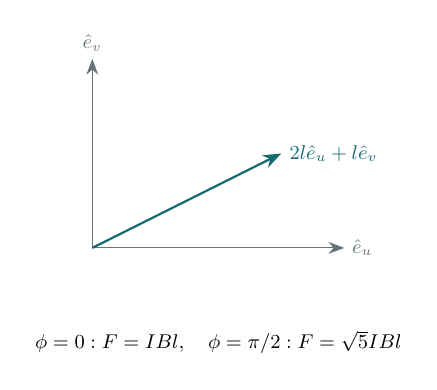
\begin{tikzpicture}[scale=.8,transform shape]
\draw[axis] (0,0)--(4,0) node[right] {$\hat e_u$};\draw[axis] (0,0)--(0,3) node[above] {$\hat e_v$};\draw[motion] (0,0)--(3,1.5) node[right] {$2l\hat e_u+l\hat e_v$};\node at (2,-1.5) {$\phi=0:F=IBl,\quad\phi=\pi/2:F=\sqrt5IBl$};
\end{tikzpicture}
\figcaption{变图电试2.4V1\quad 端点位移相对磁场的平行与垂直极限}
\end{minipage}\end{center}

\Needspace{20\baselineskip}
\item 改变内部电阻时，分别保持总电流或端电压不变，说明总力的变化，并求给定电阻的端电压表达式。
\textbf{解：}变图电试2.4V2中端点与磁场不变，固定$I$就固定$\boldsymbol F=I\Delta\boldsymbol r\times\boldsymbol B$，内部各电流可以重新分配。给定电阻的结点解有$V_a-V_d=203IR/59$，所以固定端电压$U$时$I=59U/(203R)$，$F=59\sqrt3\,UBl/(203R)$。不同电阻网络改变等效电阻，从而通过总电流改变力；两类实验保持的电量分别是$I$与$U$。
\begin{center}\begin{minipage}{.98\linewidth}\centering
\begin{tikzpicture}[scale=.8,transform shape]
\node[draw,minimum width=3cm,minimum height=1.5cm] (r) at (2,1) {$R_{\rm eq}=203R/59$};\draw[motion] (-1,1)--(r) node[midway,above] {$I$};\draw[motion] (r)--(5,1);\node at (2,-1) {恒压：$I=59U/(203R)$};
\end{tikzpicture}
\figcaption{变图电试2.4V2\quad 内部电阻通过给定的电源条件决定总电流}
\end{minipage}\end{center}

\Needspace{20\baselineskip}
\item 除$d$端外，再从$c$端抽出电流$I_c=\alpha I$，$0\le\alpha\le1$，求网络合力。
\textbf{解：}变图电试2.4V3中输出端为$c,d$，由结点消项得$\boldsymbol F=[I_c(\boldsymbol r_c-\boldsymbol r_a)+(I-I_c)(\boldsymbol r_d-\boldsymbol r_a)]\times\boldsymbol B$。代入位移，等效向量为$Il[(2-\alpha)\hat e_u+\hat e_v]$，因此$\boldsymbol F=IBl[\sin\phi\hat e_u-(2-\alpha)\sin\phi\hat e_v-\cos\phi\hat n]$，大小$IBl\sqrt{1+(2-\alpha)^2\sin^2\phi}$。多端口按每个端口电流与位置加权，内部结点仍相消。
\begin{center}\begin{minipage}{.98\linewidth}\centering
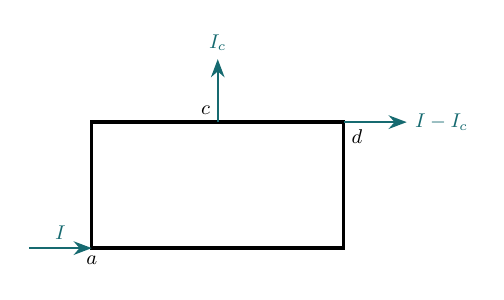
\begin{tikzpicture}[scale=.8,transform shape]
\draw[very thick] (0,0)--(0,2)--(2,2)--(4,2)--(4,0)--cycle;\draw[motion] (-1,0)--(0,0) node[midway,above] {$I$};\draw[motion] (2,2)--(2,3) node[above] {$I_c$};\draw[motion] (4,2)--(5,2) node[right] {$I-I_c$};\node[below] at (0,0) {$a$};\node[above left] at (2,2) {$c$};\node[below right] at (4,2) {$d$};
\end{tikzpicture}
\figcaption{变图电试2.4V3\quad 多输出端口按位置与电流分别加权}
\end{minipage}\end{center}

\Needspace{20\baselineskip}
\item 闭合小环处于缓慢变化的非均匀磁场，说明端点相同的两条电流路径为何可有不同合力。
\textbf{解：}变图电试2.4V4取小环磁矩$\boldsymbol m$，在环尺度上将外场按位置展开。均匀项的合力由$\oint\mathrm d\boldsymbol l=0$相消，梯度项留下$\boldsymbol F\simeq\nabla(\boldsymbol m\cdot\boldsymbol B)$。例如平面小环的$\boldsymbol m=m_z\hat n$、$B_n=B_0+Gu$，则$F_u=m_zG$。端点相同的两条路径之差是闭合环，场梯度使它产生非零合力；当$G=0$时恢复匀强场端点等效。
\begin{center}\begin{minipage}{.98\linewidth}\centering
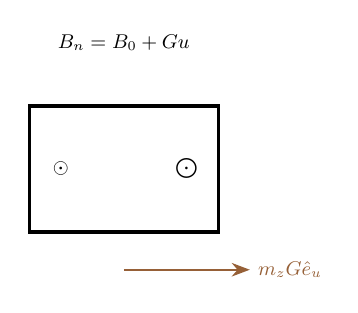
\begin{tikzpicture}[scale=.8,transform shape]
\draw[very thick] (0,0) rectangle (3,2);\node at (.5,1) {$\odot$};\node at (2.5,1) {$\bigodot$};\draw[force] (1.5,-.6)--(3.5,-.6) node[right] {$m_zG\hat e_u$};\node at (1.5,3) {$B_n=B_0+Gu$};
\end{tikzpicture}
\figcaption{变图电试2.4V4\quad 缓变非均匀场的梯度项给闭合小环净力}
\end{minipage}\end{center}

\Needspace{20\baselineskip}
\item 在右侧单位方环$f\to c\to d\to e\to f$叠加环流$J$，求总力与总力矩的变化。
\textbf{解：}变图电试2.4V5中该环流不改变端口电流，且闭合位移积分为零，所以附加合力为零。该方向在$\hat e_u,\hat e_v$平面内为顺时针，附加磁矩为$\Delta\boldsymbol m=-Jl^2\hat n$。因此力矩改变$\Delta\boldsymbol\tau=\Delta\boldsymbol m\times\boldsymbol B=-JBl^2\cos\phi\hat e_v$。相同的端点力可以伴随不同的力矩分布，图中的闭合环流具体给出了这个附加转动作用。
\begin{center}\begin{minipage}{.98\linewidth}\centering
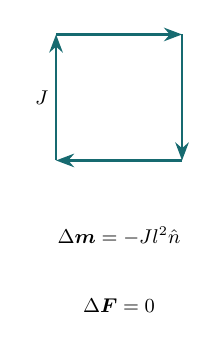
\begin{tikzpicture}[scale=.8,transform shape]
\draw[motion] (0,0)--(0,2);\draw[motion] (0,2)--(2,2);\draw[motion] (2,2)--(2,0);\draw[motion] (2,0)--(0,0);\node[left] at (0,1) {$J$};\node at (1,-1.2) {$\Delta\boldsymbol m=-Jl^2\hat n$};\node at (1,-2.3) {$\Delta\boldsymbol F=0$};
\end{tikzpicture}
\figcaption{变图电试2.4V5\quad 附加闭合环流保持总力，却改变磁力矩}
\end{minipage}\end{center}

\Needspace{20\baselineskip}
\item 把若干直支路改成同端点的弯曲导线，磁场仍均匀，总电流相同，求合力怎样变化。
\textbf{解：}变图电试2.4V6中任一弯曲支路从$i$到$j$，电流沿线保持$I_{ij}$，其合力$\int_i^jI_{ij}\mathrm d\boldsymbol l\times\boldsymbol B=I_{ij}(\boldsymbol r_j-\boldsymbol r_i)\times\boldsymbol B$。因此支路形状改变后，原有结点消项关系继续成立，网络总力保持$I(\boldsymbol r_d-\boldsymbol r_a)\times\boldsymbol B$。曲线的不同部分有不同局部力方向，合力由积分后的位移确定，局部弯曲受力与力矩可另按实际线形计算。
\begin{center}\begin{minipage}{.98\linewidth}\centering
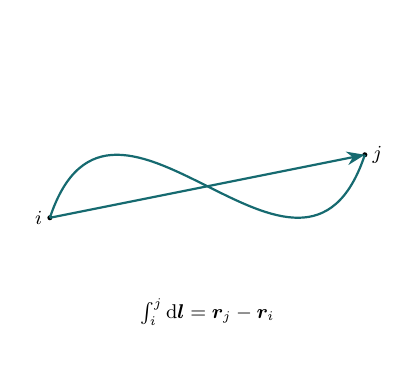
\begin{tikzpicture}[scale=.8,transform shape]
\fill (0,0) circle(.04) node[left] {$i$};\fill (5,1) circle(.04) node[right] {$j$};\draw[traj] (0,0)..controls(1,3)and(4,-2)..(5,1);\draw[motion] (0,0)--(5,1);\node at (2.5,-1.5) {$\int_i^j\mathrm d\boldsymbol l=\boldsymbol r_j-\boldsymbol r_i$};
\end{tikzpicture}
\figcaption{变图电试2.4V6\quad 弯曲支路的位移积分仍由两个端点确定}
\end{minipage}\end{center}

\Needspace{20\baselineskip}
\item 全部电阻按相同比例$h>0$增大，分别保持总电流、端电压和总焦耳功率不变，比较总磁力。
\textbf{解：}变图电试2.4V7中等效电阻从$R_{\rm eq}=203R/59$变为$hR_{\rm eq}$，支路电流比例保持相同。总力与$I$成正比，所以恒流时不变；恒压时$I'=I/h$，力变为$F/h$；恒定焦耳功率$P=I^2R_{\rm eq}$时$I'=I/\sqrt h$，力变为$F/\sqrt h$。每种条件都先用对应电学约束求总电流，再按同一空间位移计算磁场力。
\begin{center}\begin{minipage}{.98\linewidth}\centering
\begin{tikzpicture}[scale=.8,transform shape]
\draw[axis] (0,0)--(10.7,0) node[right] {$h$};
\draw[axis] (0,0)--(0,3.2) node[above] {$F'/F$};\foreach \y/\lab in {0/0,1.4/1,2.8/2}{\draw[thin] (0,\y)--(-.08,\y) node[left] {$\lab$};}
\node[above] at (5,3.5) {全部电阻同比改变：恒流、恒压、恒功率};
\draw[traj] plot coordinates {(0.000000000,1.400000000) (0.083333333,1.400000000) (0.166666667,1.400000000) (0.250000000,1.400000000) (0.333333333,1.400000000) (0.416666667,1.400000000) (0.500000000,1.400000000) (0.583333333,1.400000000) (0.666666667,1.400000000) (0.750000000,1.400000000) (0.833333333,1.400000000) (0.916666667,1.400000000) (1.000000000,1.400000000) (1.083333333,1.400000000) (1.166666667,1.400000000) (1.250000000,1.400000000) (1.333333333,1.400000000) (1.416666667,1.400000000) (1.500000000,1.400000000) (1.583333333,1.400000000) (1.666666667,1.400000000) (1.750000000,1.400000000) (1.833333333,1.400000000) (1.916666667,1.400000000) (2.000000000,1.400000000) (2.083333333,1.400000000) (2.166666667,1.400000000) (2.250000000,1.400000000) (2.333333333,1.400000000) (2.416666667,1.400000000) (2.500000000,1.400000000) (2.583333333,1.400000000) (2.666666667,1.400000000) (2.750000000,1.400000000) (2.833333333,1.400000000) (2.916666667,1.400000000) (3.000000000,1.400000000) (3.083333333,1.400000000) (3.166666667,1.400000000) (3.250000000,1.400000000) (3.333333333,1.400000000) (3.416666667,1.400000000) (3.500000000,1.400000000) (3.583333333,1.400000000) (3.666666667,1.400000000) (3.750000000,1.400000000) (3.833333333,1.400000000) (3.916666667,1.400000000) (4.000000000,1.400000000) (4.083333333,1.400000000) (4.166666667,1.400000000) (4.250000000,1.400000000) (4.333333333,1.400000000) (4.416666667,1.400000000) (4.500000000,1.400000000) (4.583333333,1.400000000) (4.666666667,1.400000000) (4.750000000,1.400000000) (4.833333333,1.400000000) (4.916666667,1.400000000) (5.000000000,1.400000000) (5.083333333,1.400000000) (5.166666667,1.400000000) (5.250000000,1.400000000) (5.333333333,1.400000000) (5.416666667,1.400000000) (5.500000000,1.400000000) (5.583333333,1.400000000) (5.666666667,1.400000000) (5.750000000,1.400000000) (5.833333333,1.400000000) (5.916666667,1.400000000) (6.000000000,1.400000000) (6.083333333,1.400000000) (6.166666667,1.400000000) (6.250000000,1.400000000) (6.333333333,1.400000000) (6.416666667,1.400000000) (6.500000000,1.400000000) (6.583333333,1.400000000) (6.666666667,1.400000000) (6.750000000,1.400000000) (6.833333333,1.400000000) (6.916666667,1.400000000) (7.000000000,1.400000000) (7.083333333,1.400000000) (7.166666667,1.400000000) (7.250000000,1.400000000) (7.333333333,1.400000000) (7.416666667,1.400000000) (7.500000000,1.400000000) (7.583333333,1.400000000) (7.666666667,1.400000000) (7.750000000,1.400000000) (7.833333333,1.400000000) (7.916666667,1.400000000) (8.000000000,1.400000000) (8.083333333,1.400000000) (8.166666667,1.400000000) (8.250000000,1.400000000) (8.333333333,1.400000000) (8.416666667,1.400000000) (8.500000000,1.400000000) (8.583333333,1.400000000) (8.666666667,1.400000000) (8.750000000,1.400000000) (8.833333333,1.400000000) (8.916666667,1.400000000) (9.000000000,1.400000000) (9.083333333,1.400000000) (9.166666667,1.400000000) (9.250000000,1.400000000) (9.333333333,1.400000000) (9.416666667,1.400000000) (9.500000000,1.400000000) (9.583333333,1.400000000) (9.666666667,1.400000000) (9.750000000,1.400000000) (9.833333333,1.400000000) (9.916666667,1.400000000) (10.000000000,1.400000000)};
\draw[dashed,thick,color=warm] plot coordinates {(0.000000000,2.800000000) (0.083333333,2.688000000) (0.166666667,2.584615385) (0.250000000,2.488888889) (0.333333333,2.400000000) (0.416666667,2.317241379) (0.500000000,2.240000000) (0.583333333,2.167741935) (0.666666667,2.100000000) (0.750000000,2.036363636) (0.833333333,1.976470588) (0.916666667,1.920000000) (1.000000000,1.866666667) (1.083333333,1.816216216) (1.166666667,1.768421053) (1.250000000,1.723076923) (1.333333333,1.680000000) (1.416666667,1.639024390) (1.500000000,1.600000000) (1.583333333,1.562790698) (1.666666667,1.527272727) (1.750000000,1.493333333) (1.833333333,1.460869565) (1.916666667,1.429787234) (2.000000000,1.400000000) (2.083333333,1.371428571) (2.166666667,1.344000000) (2.250000000,1.317647059) (2.333333333,1.292307692) (2.416666667,1.267924528) (2.500000000,1.244444444) (2.583333333,1.221818182) (2.666666667,1.200000000) (2.750000000,1.178947368) (2.833333333,1.158620690) (2.916666667,1.138983051) (3.000000000,1.120000000) (3.083333333,1.101639344) (3.166666667,1.083870968) (3.250000000,1.066666667) (3.333333333,1.050000000) (3.416666667,1.033846154) (3.500000000,1.018181818) (3.583333333,1.002985075) (3.666666667,0.988235294) (3.750000000,0.973913043) (3.833333333,0.960000000) (3.916666667,0.946478873) (4.000000000,0.933333333) (4.083333333,0.920547945) (4.166666667,0.908108108) (4.250000000,0.896000000) (4.333333333,0.884210526) (4.416666667,0.872727273) (4.500000000,0.861538462) (4.583333333,0.850632911) (4.666666667,0.840000000) (4.750000000,0.829629630) (4.833333333,0.819512195) (4.916666667,0.809638554) (5.000000000,0.800000000) (5.083333333,0.790588235) (5.166666667,0.781395349) (5.250000000,0.772413793) (5.333333333,0.763636364) (5.416666667,0.755056180) (5.500000000,0.746666667) (5.583333333,0.738461538) (5.666666667,0.730434783) (5.750000000,0.722580645) (5.833333333,0.714893617) (5.916666667,0.707368421) (6.000000000,0.700000000) (6.083333333,0.692783505) (6.166666667,0.685714286) (6.250000000,0.678787879) (6.333333333,0.672000000) (6.416666667,0.665346535) (6.500000000,0.658823529) (6.583333333,0.652427184) (6.666666667,0.646153846) (6.750000000,0.640000000) (6.833333333,0.633962264) (6.916666667,0.628037383) (7.000000000,0.622222222) (7.083333333,0.616513761) (7.166666667,0.610909091) (7.250000000,0.605405405) (7.333333333,0.600000000) (7.416666667,0.594690265) (7.500000000,0.589473684) (7.583333333,0.584347826) (7.666666667,0.579310345) (7.750000000,0.574358974) (7.833333333,0.569491525) (7.916666667,0.564705882) (8.000000000,0.560000000) (8.083333333,0.555371901) (8.166666667,0.550819672) (8.250000000,0.546341463) (8.333333333,0.541935484) (8.416666667,0.537600000) (8.500000000,0.533333333) (8.583333333,0.529133858) (8.666666667,0.525000000) (8.750000000,0.520930233) (8.833333333,0.516923077) (8.916666667,0.512977099) (9.000000000,0.509090909) (9.083333333,0.505263158) (9.166666667,0.501492537) (9.250000000,0.497777778) (9.333333333,0.494117647) (9.416666667,0.490510949) (9.500000000,0.486956522) (9.583333333,0.483453237) (9.666666667,0.480000000) (9.750000000,0.476595745) (9.833333333,0.473239437) (9.916666667,0.469930070) (10.000000000,0.466666667)};
\draw[guide] plot coordinates {(0.000000000,1.979898987) (0.083333333,1.939896904) (0.166666667,1.902225417) (0.250000000,1.866666667) (0.333333333,1.833030278) (0.416666667,1.801149059) (0.500000000,1.770875490) (0.583333333,1.742078847) (0.666666667,1.714642820) (0.750000000,1.688463530) (0.833333333,1.663447872) (0.916666667,1.639512123) (1.000000000,1.616580754) (1.083333333,1.594585433) (1.166666667,1.573464163) (1.250000000,1.553160549) (1.333333333,1.533623161) (1.416666667,1.514804986) (1.500000000,1.496662955) (1.583333333,1.479157523) (1.666666667,1.462252310) (1.750000000,1.445913783) (1.833333333,1.430110972) (1.916666667,1.414815227) (2.000000000,1.400000000) (2.083333333,1.385640646) (2.166666667,1.371714256) (2.250000000,1.358199500) (2.333333333,1.345076492) (2.416666667,1.332326664) (2.500000000,1.319932658) (2.583333333,1.307878226) (2.666666667,1.296148140) (2.750000000,1.284728110) (2.833333333,1.273604713) (2.916666667,1.262765327) (3.000000000,1.252198067) (3.083333333,1.241891735) (3.166666667,1.231835766) (3.250000000,1.222020185) (3.333333333,1.212435565) (3.416666667,1.203072988) (3.500000000,1.193924012) (3.583333333,1.184980635) (3.666666667,1.176235271) (3.750000000,1.167680719) (3.833333333,1.159310140) (3.916666667,1.151117033) (4.000000000,1.143095213) (4.083333333,1.135238796) (4.166666667,1.127542173) (4.250000000,1.120000000) (4.333333333,1.112607180) (4.416666667,1.105358848) (4.500000000,1.098250357) (4.583333333,1.091277268) (4.666666667,1.084435337) (4.750000000,1.077720502) (4.833333333,1.071128878) (4.916666667,1.064656741) (5.000000000,1.058300524) (5.083333333,1.052056809) (5.166666667,1.045922315) (5.250000000,1.039893894) (5.333333333,1.033968524) (5.416666667,1.028143303) (5.500000000,1.022415441) (5.583333333,1.016782255) (5.666666667,1.011241166) (5.750000000,1.005789691) (5.833333333,1.000425441) (5.916666667,0.995146115) (6.000000000,0.989949494) (6.083333333,0.984833441) (6.166666667,0.979795897) (6.250000000,0.974834873) (6.333333333,0.969948452) (6.416666667,0.965134783) (6.500000000,0.960392077) (6.583333333,0.955718608) (6.666666667,0.951112709) (6.750000000,0.946572765) (6.833333333,0.942097219) (6.916666667,0.937684561) (7.000000000,0.933333333) (7.083333333,0.929042123) (7.166666667,0.924809563) (7.250000000,0.920634329) (7.333333333,0.916515139) (7.416666667,0.912450750) (7.500000000,0.908439958) (7.583333333,0.904481595) (7.666666667,0.900574529) (7.750000000,0.896717661) (7.833333333,0.892909926) (7.916666667,0.889150288) (8.000000000,0.885437745) (8.083333333,0.881771320) (8.166666667,0.878150067) (8.250000000,0.874573067) (8.333333333,0.871039424) (8.416666667,0.867548270) (8.500000000,0.864098760) (8.583333333,0.860690073) (8.666666667,0.857321410) (8.750000000,0.853991994) (8.833333333,0.850701068) (8.916666667,0.847447897) (9.000000000,0.844231765) (9.083333333,0.841051973) (9.166666667,0.837907842) (9.250000000,0.834798712) (9.333333333,0.831723936) (9.416666667,0.828682888) (9.500000000,0.825674954) (9.583333333,0.822699540) (9.666666667,0.819756061) (9.750000000,0.816843952) (9.833333333,0.813962660) (9.916666667,0.811111643) (10.000000000,0.808290377)};
\node[below] at (0,-.12) {$0.5$};
\node[below] at (2,-.12) {$1$};
\node[below] at (10,-.12) {$3$};
\end{tikzpicture}
\figcaption{变图电试2.4V7\quad 实线为恒流，虚线为恒压，点线为恒功率。}
\end{minipage}\end{center}

\Needspace{20\baselineskip}
\item 在$\phi=45^\circ$时，求合力与网络平面的夹角。
\textbf{解：}变图电试2.4V8中$\boldsymbol F=(IBl/\sqrt2)(\hat e_u-2\hat e_v-\hat n)$。面内分量大小为$IBl\sqrt{5/2}$，法向分量大小为$IBl/\sqrt2$，总大小为$\sqrt3IBl$。因此与平面的夹角$\psi$满足$\tan\psi=1/\sqrt5$，等价地$\sin\psi=1/\sqrt6$，即约24.1度。法向分量沿$-\hat n$，面内分量沿$\hat e_u-2\hat e_v$，这两个方向共同确定三维合力。
\begin{center}\begin{minipage}{.98\linewidth}\centering
\begin{tikzpicture}[scale=.8,transform shape]
\draw[axis] (0,0)--(4,0) node[right] {面内};\draw[axis] (0,0)--(0,-2.5) node[below] {$-\hat n$};\draw[motion] (0,0)--(3,-1.341641) node[right] {$\boldsymbol F$};\draw[guide] (3,0)--(3,-1.341641)--(0,-1.341641);\node at (2,1) {$\tan\psi=1/\sqrt5$};
\end{tikzpicture}
\figcaption{变图电试2.4V8\quad 总力的面内与法向分量确定其倾角}
\end{minipage}\end{center}
\end{enumerate}

\Needspace{13\baselineskip}

\pdfbookmark[2]{第 5 题 时变磁场中带电弦杆的转动与端点作用力}{q5}

\section*{第 5 题\quad 时变磁场中带电弦杆的转动与端点作用力}\label{q:5}


半径$R$的光滑绝缘圆环固定在水平面内。以环为横截面的竖直圆柱区域内有磁场
$\boldsymbol B=-B(t)\hat z$，其中$B(t)=B_0\sin\omega_0t$、$B_0>0$，$\hat z$竖直向上；柱外磁场为零。采用轴对称的感应电场，忽略附加静电场、自场和辐射。
均匀绝缘刚性细杆$ab$总质量$m$、总正电荷$Q$，其质心$C$距环心$O$为$D=R/2$，两端由光滑的双向径向约束保持在圆周上。电荷分布始终均匀；重力由水平支承平衡，只求水平面内作用力。
$t=0$时杆静止，此后先逆时针转过$2\pi$，再顺时针返回$2\pi$，如此交替。
\begin{enumerate}
\item 求$\omega_0$与$m,Q,B_0$的关系。
\item 求杆在$a,b$端对约束圆环的水平作用力随时间的变化，给出大小和实际方向。
\item 说明上述双向约束若改为只能向杆施加朝向$O$压力的普通单侧内壁，给定运动能否实现。
\end{enumerate}
令$\hat e_r$由$O$指向$C$，$\hat e_t=\hat z\times\hat e_r$；初始杆沿$\hat e_t$，$a$在$C$的负$\hat e_t$侧，$b$在正侧。


\begin{center}\begin{minipage}{.98\linewidth}\centering
\begin{tikzpicture}[scale=.75,transform shape]

\draw[object] (0,0) circle (2);
\draw[object,line width=1.5pt] (1,-1.732)--(1,1.732);
\fill (0,0) circle (1.5pt) node[below left] {$O$};
\fill[color=accent] (1,0) circle (2pt) node[below right] {$C$};
\node[below right] at (1,-1.732) {$a$};
\node[above right] at (1,1.732) {$b$};
\draw[guide] (0,0)--(1,0) node[midway,below] {$D$};
\draw[guide] (0,0)--(1,1.732) node[midway,above left] {$R$};

\draw[axis] (0,0)--(2.7,0) node[right] {$\hat e_r$};
\draw[axis] (1,.15)--(1,2.5) node[above] {$\hat e_t$};
\node at (-1,1) {$\otimes\ B(t)$};
\node at (0,-2.6) {$D=R/2,\quad L=\sqrt3D$};
\node[align=left] at (4.8,1) {杆：均匀$m,Q$\\初始静止\\端点双向径向约束};

\end{tikzpicture}
\figcaption{图电试2.5\quad 俯视水平圆环，a、b的标记随杆运动而保持。}
\end{minipage}\end{center}

\Needspace{8\baselineskip}

\pdfbookmark[3]{题型定位}{q5-h0}

\subsection*{题型定位}

时变磁场通过感应电场驱动均匀带电刚体。以固定环心的转动方程求角速度和连续转角，再以质心平动方程求两端反力。支承方式决定反力能否实现，杆对环与环对杆的力按作用对象分别给出。均匀电荷与质量分布使二次矩具有同一个几何因子，形成清楚的转动关系。

\Needspace{8\baselineskip}

\pdfbookmark[3]{知识点}{q5-h1}

\subsection*{知识点}

轴对称法拉第电场为$\boldsymbol E=(\dot B/2)\hat z\times\boldsymbol r$，符号跟随$\dot B$。杆的固定轴惯量含质心自转项与平行轴项，电场力矩按每个电荷元到固定轴的距离平方积分。磁力逐点通过环心，合力仍参与质心向心运动。两端径向反力由径向与切向方程联立，再按牛顿第三定律得到杆对环作用力。

\Needspace{8\baselineskip}

\pdfbookmark[3]{物理图像}{q5-h2}

\subsection*{物理图像}

题图给出偏心距$D$、半弦长$L$和两个端点。解图电试2.5A把$+s,-s$电荷元配对，感应电场径向分量相消、切向分量相加，电场力矩同号。图B保留连续转角从0增到$2\pi$再回到0的全过程。图C在端点实际画出环对杆向外、杆对环向内的两个对象，二者合力各自沿质心半径方向。

\Needspace{8\baselineskip}

\pdfbookmark[3]{解题入口}{q5-h3}

\subsection*{解题入口}

先用$\boldsymbol r=D\hat e_r+s\hat e_t$同时表示质量元和电荷元位置，把惯量与电场力矩的共同几何积分写出。转动方程给$\dot\Omega=Q\dot B/(2m)$，零初值积分后由最大连续转角求驱动频率。反力计算回到质心方程，感应电场恰好提供所需切向力，磁力超过所需向心力的部分由向外约束力平衡。

\Needspace{8\baselineskip}

\pdfbookmark[3]{标准解法}{q5-h4}

\subsection*{标准解法}


图电试2.5中半杆长记为$L$，由弦的几何关系，
\[
D=\frac R2,\qquad L=\sqrt{R^2-D^2}=\sqrt3D.
\]
杆两端在同一圆周上，连接环心与弦中点的半径垂直杆，勾股关系给$D^2+L^2=R^2$。半杆长是$L$，完整杆长是$2L$，因此均匀质量与电荷的线密度分别为$m/(2L)$与$Q/(2L)$。随杆转动的基矢为$\hat e_r,\hat e_t$。用$s\in[-L,L]$标记杆上的电荷元，则相对于固定环心$O$，
\[
\boldsymbol r=D\hat e_r+s\hat e_t,\qquad
dq=\frac Q{2L}\,ds,\quad dm=\frac m{2L}\,ds.
\]
转角$\theta$取逆时针为正，$\Omega=\dot\theta$。整根杆绕固定$O$转动，惯量由质心自转项和平行轴项相加。

运动中的每个质元既绕杆质心转动，也随质心绕环心移动，关于固定轴的速度统一写为$\Omega\hat z\times\boldsymbol r$。取这一固定轴做力矩方程，可把两个端点的径向约束力同时消去。由法拉第定律，在柱内半径$r$的圆周上，取逆时针积分方向，
\[
2\pi rE_\varphi=-\frac d{dt}(-\pi r^2B)
=\pi r^2\dot B.
\]
因此
\[
\boxed{\boldsymbol E(\boldsymbol r,t)
=\frac{\dot B}{2}\hat z\times\boldsymbol r
=\frac{\dot B}{2}(D\hat e_t-s\hat e_r)}.
\]
这是随$\dot B$变号的矢量式，感应电场方向在$\dot B$变号时反向。若取柱外$r>R$的圆周，磁通量只覆盖半径$R$的区域，法拉第定律给$E_\varphi=R^2\dot B/(2r)$；在$r=R$与柱内表达式连续。本题$|\boldsymbol r|=\sqrt{D^2+s^2}\le R$，所以全杆均使用柱内表达式，端点取其连续值。
\begin{center}\begin{minipage}{.98\linewidth}\centering
\begin{tikzpicture}[scale=.75,transform shape]

\draw[object] (0,0) circle (2);
\draw[object,line width=1.5pt] (1,-1.732)--(1,1.732);
\fill (0,0) circle (1.5pt) node[below left] {$O$};
\fill[color=accent] (1,0) circle (2pt) node[below right] {$C$};
\node[below right] at (1,-1.732) {$a$};
\node[above right] at (1,1.732) {$b$};
\draw[guide] (0,0)--(1,0) node[midway,below] {$D$};
\draw[guide] (0,0)--(1,1.732);

\fill[color=accent] (1,.9) circle (2pt) node[right] {$+s$};
\fill[color=accent] (1,-.9) circle (2pt) node[right] {$-s$};
\draw[force] (1,.9)--(.1,1.9) node[above left] {$d\boldsymbol F_E$};
\draw[force] (1,-.9)--(1.9,.1) node[right] {$d\boldsymbol F_E$};
\draw[motion] (-1.5,-1)--(-1.5,0) node[left] {$\hat e_t$};
\node[align=center] at (4.5,.9) {$E_r\propto-s$：相消\\$E_t\propto D$：相加};
\node[align=center] at (4.5,-.9) {$\tau_E=\frac{\dot B}{2}\int r^2dq$\\$d\boldsymbol F_B\parallel-\boldsymbol r$};
\node at (.8,2.8) {示例 $\dot B>0$：电场力矩逆时针};

\end{tikzpicture}
\figcaption{解图电试2.5A\quad 对称电荷元的电场力切向分量相加，径向磁力对O的矩为零。}
\end{minipage}\end{center}
解图电试2.5A画出一对$\pm s$电荷元。它们的径向感应电场力相消，切向分量相加；对$O$的力矩同号。积分得
\[
\boldsymbol F_E=\frac{QD\dot B}{2}\hat e_t,\qquad
\tau_{E,z}=\frac{\dot B}{2}\int(D^2+s^2)dq
=\frac{Q\dot B}{2}\left(D^2+\frac{L^2}{3}\right).
\]
对称积分中$\int s\,\mathrm dq=0$，$\int s^2\mathrm dq=QL^2/3$。因此电场合力只留下质心处的切向项，而力矩同时保留偏心距的$D^2$与杆内电荷分布的$L^2/3$。力矩的每个元为$[\boldsymbol r\times\boldsymbol E]_z\mathrm dq=(\dot B/2)(D^2+s^2)\mathrm dq$，在$\dot B$同号时沿杆各处具有相同方向。磁力的局部形式为
\[
\boldsymbol v=\Omega\hat z\times\boldsymbol r,\qquad
d\boldsymbol F_B=dq\,\boldsymbol v\times(-B\hat z)
=-B\Omega\,\boldsymbol r\,dq.
\]
每个磁力都通过$O$，两端径向约束力也通过$O$，对该轴均无力矩。杆对$O$的转动惯量为
\[
J=\int(D^2+s^2)dm
=m\left(D^2+\frac{L^2}{3}\right)=2mD^2.
\]
质量二次矩的积分同样用$\int s^2\mathrm dm=mL^2/3$，所以$\tau_{E,z}/J$约去相同的几何因子$D^2+L^2/3$。这里起作用的是电荷与质量具有相同的均匀分布，电荷二次矩与质量二次矩之比为$Q/m$。转动方程给
\[
J\dot\Omega=\tau_{E,z},\qquad
\dot\Omega=\frac Q{2m}\dot B.
\]
由$B(0)=0,\Omega(0)=0$，
\[
\boxed{\Omega(t)=\frac{QB_0}{2m}\sin\omega_0t,\qquad
\theta(t)=\frac{QB_0}{2m\omega_0}(1-\cos\omega_0t)}.
\]
\begin{center}\begin{minipage}{.98\linewidth}\centering
\begin{tikzpicture}[scale=.8,transform shape]

\draw[axis] (0,0)--(7.2,0) node[right] {$u=\omega_0t$};
\draw[axis] (0,-.2)--(0,2.8) node[above] {$\theta/\pi$};
\draw[traj,domain=0:12.56637,samples=140] plot ({.5*\x},{1-cos(\x r)});
\draw[guide] (0,2)--(6.5,2);
\foreach \x/\lab in {1.5708/\pi,3.14159/2\pi,4.71239/3\pi,6.28318/4\pi}
{\draw (\x,0)--(\x,-.08);\node[below] at (\x,-.08) {$\lab$};}
\node[left] at (0,2) {$2$};
\node at (1.3,2.7) {$\Omega>0$};
\node at (2.7,2.7) {$\Omega<0$};
\node at (3,-1.2) {每周期前半段逆时针，后半段顺时针};

\end{tikzpicture}
\figcaption{解图电试2.5B\quad 连续转角先增至整周再返回；极大处实际角速度为零。}
\end{minipage}\end{center}
解图电试2.5B将连续转角从$0$画到最大值再返回。$0<t<\pi/\omega_0$时$\Omega>0$，最大转角出现在$t=\pi/\omega_0$：
\[
\theta_{\max}=\frac{QB_0}{m\omega_0}=2\pi.
\]
故
\[
\boxed{\omega_0=\frac{QB_0}{2\pi m}}.
\]
代入频率关系后，$\theta=\pi(1-\cos\omega_0t)$。连续转角的中值是$\pi$，相对中值的振幅也是$\pi$，其最小、最大值分别为0与$2\pi$；实际角速度幅值则为$QB_0/(2m)=\pi\omega_0$。达到$2\pi$时杆与初始方向在几何上重合，但连续转角尚未返回零；此后$\Omega<0$，才顺时针转回。连续转角记录从起始时刻积累的转动，完整保留已经经过的一整周。

在$\omega_0t=\pi/2$时杆转到$\theta=\pi$，角速度达到正最大值；到$\omega_0t=\pi$时虽然方向与初态重合，角速度降为零，此后再反向运动。半周期之后的速度反向与连续转角的回程在图B上分别由斜率和角度表示。

第（2）问须另用质心平动方程。对磁力积分，
\[
\boldsymbol F_B=-QB\Omega D\,\hat e_r
=-2m\Omega^2D\,\hat e_r.
\]
质心的加速度为
\[
\boldsymbol a_C=-D\Omega^2\hat e_r+D\dot\Omega\hat e_t,
\qquad \boldsymbol F_E=mD\dot\Omega\hat e_t.
\]
于是由质心方程得到圆环对杆的两端合力
\[
\boldsymbol F_{N,a}+\boldsymbol F_{N,b}
=m\boldsymbol a_C-\boldsymbol F_E-\boldsymbol F_B
=mD\Omega^2\hat e_r.
\]
\begin{center}\begin{minipage}{.98\linewidth}\centering
\begin{tikzpicture}[scale=.65,transform shape]

\draw[object] (0,0) circle (2);
\draw[object,line width=1.5pt] (1,-1.732)--(1,1.732);
\fill (0,0) circle (1.5pt) node[below left] {$O$};
\fill[color=accent] (1,0) circle (2pt) node[below right] {$C$};
\node[below right] at (1,-1.732) {$a$};
\node[above right] at (1,1.732) {$b$};
\draw[guide] (0,0)--(1,0) node[midway,below] {$D$};
\draw[guide] (0,0)--(1,1.732);

\draw[force] (1,1.732)--(1.5,2.598) node[above right] {$\nu_b$};
\draw[force] (1,-1.732)--(1.5,-2.598) node[below right] {$\nu_a$};
\node at (-.8,2.8) {环对杆：向外};
\begin{scope}[xshift=6.5cm]

\draw[object] (0,0) circle (2);
\draw[object,line width=1.5pt] (1,-1.732)--(1,1.732);
\fill (0,0) circle (1.5pt) node[below left] {$O$};
\fill[color=accent] (1,0) circle (2pt) node[below right] {$C$};
\node[below right] at (1,-1.732) {$a$};
\node[above right] at (1,1.732) {$b$};
\draw[guide] (0,0)--(1,0) node[midway,below] {$D$};
\draw[guide] (0,0)--(1,1.732);

\draw[motion] (1,1.732)--(.5,.866);
\draw[motion] (1,-1.732)--(.5,-.866);
\node[left] at (.4,1.2) {$\boldsymbol N_b$};
\node[left] at (.4,-1.2) {$\boldsymbol N_a$};
\node at (0,2.8) {杆对环：向内};
\end{scope}
\node at (3,-3.7) {大小均为 $mR\Omega^2/2$；双向滑槽向杆提供向外反力};

\end{tikzpicture}
\figcaption{解图电试2.5C\quad 两幅图是一对作用与反作用，箭头沿各端点自己的半径。}
\end{minipage}\end{center}
解图电试2.5C把端点约束力取沿各自半径向外为正。端点位置为
$\boldsymbol r_a=D\hat e_r-L\hat e_t$、
$\boldsymbol r_b=D\hat e_r+L\hat e_t$，设
\[
\boldsymbol F_{N,a}=\nu_a\frac{\boldsymbol r_a}{R},
\qquad
\boldsymbol F_{N,b}=\nu_b\frac{\boldsymbol r_b}{R}.
\]
每个端点的外向单位法线都有$D/R$的$\hat e_r$分量，切向分量分别为$-L/R$与$+L/R$。因此两端反力相等时，切向分量抵消、径向分量同向相加。沿$\hat e_t$和$\hat e_r$比较：
\[
\frac L R(\nu_b-\nu_a)=0,\qquad
\frac D R(\nu_a+\nu_b)=mD\Omega^2.
\]
因此$\nu_a=\nu_b=mR\Omega^2/2$，两者对杆都实际向外。杆对圆环的作用力与此反向：
\[
\boxed{\boldsymbol N_a=-\frac{m\Omega^2}{2}\boldsymbol r_a,\qquad
\boldsymbol N_b=-\frac{m\Omega^2}{2}\boldsymbol r_b}.
\]
每个端点对环的力都指向$O$，大小为
\[
\boxed{N_a=N_b=\frac{Q^2B_0^2R}{8m}\sin^2\omega_0t}.
\]
方向随端点绕$O$转动，两力的切向分量互相抵消，沿质心半径的分量相加。若要在固定坐标中写出，初始$\hat e_r=\hat x$、$\hat e_t=\hat y$，则
\[
\begin{aligned}
\boldsymbol r_a&=(D\cos\theta+L\sin\theta)\hat x
+(D\sin\theta-L\cos\theta)\hat y,\\
\boldsymbol r_b&=(D\cos\theta-L\sin\theta)\hat x
+(D\sin\theta+L\cos\theta)\hat y.
\end{aligned}
\]
两端对环的合力为$\boldsymbol N_a+\boldsymbol N_b=-mD\Omega^2\hat e_r$，与环对杆的外向合力互为相反数。每个端点矢量都沿自己到环心的方向，端点$a,b$在固定坐标里的两个坐标分别随同一连续角度转动。将已求的$\theta(t),\Omega(t)$代入，即得两个力的完整时间函数。

两端对环的力在具体时刻还可直接读出方向。例如$\omega_0t=\pi/2$时$\theta=\pi$，$a,b$分别在$-D\hat x+L\hat y$与$-D\hat x-L\hat y$，所以
\[
\boldsymbol N_a=\frac{m\Omega_{\max}^2}{2}(D\hat x-L\hat y),\qquad
\boldsymbol N_b=\frac{m\Omega_{\max}^2}{2}(D\hat x+L\hat y).
\]
两力在水平面内沿$\hat y$的分量相消、沿$+\hat x$的分量相加，共同指向环心一侧；在$\omega_0t=3\pi/2$，同名端点回到相同位置，角速度反向而力矢量相同。

第（3）问中，普通单侧内壁向杆提供朝向环心的压力，而保持弦位置所需的约束合力沿径向向外。当$\Omega\ne0$时，普通内壁失去接触；捕获式滑槽可沿两个径向方向施力，提供上述双向约束模型所需的端点反力。

感应电场的能量交换可由功率写出。约束力沿半径、端点速度沿切线，均不做功；磁力也不做功。感应电场功率为
\[
P_E=\int\boldsymbol E\cdot\boldsymbol v\,dq
=\tau_{E,z}\Omega
=J\dot\Omega\,\Omega
=\frac d{dt}\left(\frac12J\Omega^2\right).
\]
功率正负由$\Omega\dot\Omega$决定。在驱动相位$0$至$\pi/2$、$\pi$至$3\pi/2$，角速度的绝对值增大，电场输入动能；在另两个四分之一周期中，角速度的绝对值减小，电场取回动能。整周期末角速度与动能回到初态，净电场功为零。本题的动能和功率还可写为
\[
K=\frac{Q^2B_0^2R^2}{16m}\sin^2\omega_0t,\qquad
P_E=\frac{Q^2B_0^2R^2\omega_0}{8m}\sin\omega_0t\cos\omega_0t.
\]
动能峰值出现在连续转角为$\pi$的两个时刻，最大连续转角处则因角速度为零而动能为零。电场在每次转向前取回动能，再沿相反方向重新输入，完整记录了往返转动的能量交换。


\Needspace{8\baselineskip}

\pdfbookmark[3]{关键洞察}{q5-h5}

\subsection*{关键洞察}

力对固定环心无矩，只说明它在该轴的转动方程中消失；同一个磁力的合力在质心方程中达到所需向心力的两倍。于是环对杆需提供向外合力，两个端点的切向分量相消、径向分量相加。双向滑槽可以实现这个反力，普通内壁则提供相反类型的单侧压力。

\Needspace{8\baselineskip}

\pdfbookmark[3]{易错点}{q5-h6}

\subsection*{易错点}

惯量用关于固定环心的$J=m(D^2+L^2/3)$，电场力矩也积分到同一轴。感应电场随$\dot B$变号，磁力由$B\Omega$决定方向；本题$\Omega=QB/(2m)$使它始终向心。连续转角与几何方向分开记录，驱动频率$\omega_0$与实际角速度$\Omega(t)$分别使用。端点力先说明是谁对谁，再给矢量和非负大小；约束装置按所得实际方向选取。

\Needspace{8\baselineskip}

\pdfbookmark[3]{课堂讲解建议}{q5-h7}

\subsection*{课堂讲解建议}

先把杆的自转与质心绕环心运动同时画出，写出固定轴惯量，再比较电荷二次矩，解释两者为何约去同一个几何因子。用法拉第积分确定感应场的带符号方向，两次时间积分各自代入初值。

画连续转角时标0、$\pi$、$2\pi$和角速度正负，在四分之一驱动周期处同时读出角度、角速度、动能与端点力。求反力后逐个箭头说明作用对象，再换成单侧内壁，由质心所缺少的向外力说明脱离后的径向运动。最后用电场功率与动能变化对应四段加速、减速过程。

\Needspace{8\baselineskip}

\pdfbookmark[3]{变式训练}{q5-h8}

\subsection*{变式训练}

\begin{enumerate}
\Needspace{20\baselineskip}
\item 将偏心距改为一般$0<D<R$，求驱动频率和两端作用力是否改变。
\textbf{解：}变图电试2.5V1中半弦长$L=\sqrt{R^2-D^2}$。均匀质量、电荷的二次矩分别为$J=m(D^2+L^2/3)$与$J_q=Q(D^2+L^2/3)$，故$J\dot\Omega=(\dot B/2)J_q$仍给$\Omega=QB/(2m)$。最大转角条件仍得$\omega_0=QB_0/(2\pi m)$。质心方程的向外约束合力为$mD\Omega^2\hat e_r$，两端力的径向分量各含$D/R$，由此每端大小仍为$mR\Omega^2/2$。偏心距同时进入合力和方向投影，两者相除后约去。
\begin{center}\begin{minipage}{.98\linewidth}\centering
\begin{tikzpicture}[scale=.8,transform shape]
\draw[very thick] (0,0) circle (2);\draw[very thick,color=accent] (.8,-1.833030278)--(.8,1.833030278);\fill (0,0) circle(.04) node[left] {$O$};\fill (.8,0) circle(.04) node[right] {$C$};\draw[<->] (0,-.4)--(.8,-.4) node[midway,below] {$D$};\node at (0,-3) {$L^2+D^2=R^2,\quad0<D<R$};
\end{tikzpicture}
\figcaption{变图电试2.5V1\quad 一般偏心距下的质量与电荷二次矩}
\end{minipage}\end{center}

\Needspace{20\baselineskip}
\item 初始角速度为$\Omega_i$、初始磁场为$B_i$，写角运动的一般积分。
\textbf{解：}变图电试2.5V2中$\dot\Omega=Q\dot B/(2m)$，所以$\Omega(t)=\Omega_i+Q[B(t)-B_i]/(2m)$。再积分得$\theta(t)-\theta(0)=\Omega_it+(Q/2m)[\int_0^tB(t')\mathrm dt'-B_it]$。若$B=B_0\sin\omega_0t$且$B_i=0$，角度含$\Omega_it$的线性漂移；一个磁场周期后净角位移为$2\pi\Omega_i/\omega_0$。零初速使这个漂移项消失，才形成题设的往返角运动。
\begin{center}\begin{minipage}{.98\linewidth}\centering
\begin{tikzpicture}[scale=.8,transform shape]
\draw[axis] (0,0)--(10.7,0) node[right] {$\tau=\omega_0t$};
\draw[axis] (0,0)--(0,3.2) node[above] {$2m\omega_0\theta/(QB_0)$};\foreach \y/\lab in {0/0,0.85/1,1.7/2,2.55/3}{\draw[thin] (0,\y)--(-.08,\y) node[left] {$\lab$};}
\node[above] at (5,3.5) {非零初速叠加连续转角的线性漂移};
\draw[traj] plot coordinates {(0.000000000,0.000000000) (0.062500000,0.007331204) (0.125000000,0.015972035) (0.187500000,0.025919465) (0.250000000,0.037168448) (0.312500000,0.049711934) (0.375000000,0.063540874) (0.437500000,0.078644240) (0.500000000,0.095009036) (0.562500000,0.112620324) (0.625000000,0.131461241) (0.687500000,0.151513031) (0.750000000,0.172755067) (0.812500000,0.195164891) (0.875000000,0.218718242) (0.937500000,0.243389095) (1.000000000,0.269149705) (1.062500000,0.295970643) (1.125000000,0.323820848) (1.187500000,0.352667670) (1.250000000,0.382476924) (1.312500000,0.413212938) (1.375000000,0.444838615) (1.437500000,0.477315484) (1.500000000,0.510603761) (1.562500000,0.544662412) (1.625000000,0.579449214) (1.687500000,0.614920823) (1.750000000,0.651032838) (1.812500000,0.687739870) (1.875000000,0.724995614) (1.937500000,0.762752918) (2.000000000,0.800963855) (2.062500000,0.839579802) (2.125000000,0.878551510) (2.187500000,0.917829180) (2.250000000,0.957362543) (2.312500000,0.997100935) (2.375000000,1.036993375) (2.437500000,1.076988648) (2.500000000,1.117035376) (2.562500000,1.157082103) (2.625000000,1.197077376) (2.687500000,1.236969817) (2.750000000,1.276708208) (2.812500000,1.316241571) (2.875000000,1.355519241) (2.937500000,1.394490949) (3.000000000,1.433106896) (3.062500000,1.471317834) (3.125000000,1.509075137) (3.187500000,1.546330881) (3.250000000,1.583037913) (3.312500000,1.619149928) (3.375000000,1.654621537) (3.437500000,1.689408339) (3.500000000,1.723466990) (3.562500000,1.756755267) (3.625000000,1.789232136) (3.687500000,1.820857813) (3.750000000,1.851593827) (3.812500000,1.881403081) (3.875000000,1.910249903) (3.937500000,1.938100108) (4.000000000,1.964921046) (4.062500000,1.990681656) (4.125000000,2.015352509) (4.187500000,2.038905860) (4.250000000,2.061315684) (4.312500000,2.082557721) (4.375000000,2.102609510) (4.437500000,2.121450427) (4.500000000,2.139061715) (4.562500000,2.155426511) (4.625000000,2.170529877) (4.687500000,2.184358818) (4.750000000,2.196902303) (4.812500000,2.208151286) (4.875000000,2.218098716) (4.937500000,2.226739548) (5.000000000,2.234070751) (5.062500000,2.240091316) (5.125000000,2.244802254) (5.187500000,2.248206593) (5.250000000,2.250309378) (5.312500000,2.251117661) (5.375000000,2.250640490) (5.437500000,2.248888893) (5.500000000,2.245875865) (5.562500000,2.241616346) (5.625000000,2.236127198) (5.687500000,2.229427177) (5.750000000,2.221536909) (5.812500000,2.212478854) (5.875000000,2.202277272) (5.937500000,2.190958187) (6.000000000,2.178549347) (6.062500000,2.165080177) (6.125000000,2.150581741) (6.187500000,2.135086688) (6.250000000,2.118629203) (6.312500000,2.101244957) (6.375000000,2.082971049) (6.437500000,2.063845949) (6.500000000,2.043909441) (6.562500000,2.023202559) (6.625000000,2.001767525) (6.687500000,1.979647685) (6.750000000,1.956887439) (6.812500000,1.933532175) (6.875000000,1.909628200) (6.937500000,1.885222666) (7.000000000,1.860363497) (7.062500000,1.835099318) (7.125000000,1.809479380) (7.187500000,1.783553478) (7.250000000,1.757371884) (7.312500000,1.730985261) (7.375000000,1.704444589) (7.437500000,1.677801086) (7.500000000,1.651106127) (7.562500000,1.624411168) (7.625000000,1.597767664) (7.687500000,1.571226992) (7.750000000,1.544840369) (7.812500000,1.518658775) (7.875000000,1.492732874) (7.937500000,1.467112935) (8.000000000,1.441848757) (8.062500000,1.416989588) (8.125000000,1.392584053) (8.187500000,1.368680078) (8.250000000,1.345324815) (8.312500000,1.322564568) (8.375000000,1.300444728) (8.437500000,1.279009694) (8.500000000,1.258302812) (8.562500000,1.238366304) (8.625000000,1.219241205) (8.687500000,1.200967296) (8.750000000,1.183583050) (8.812500000,1.167125566) (8.875000000,1.151630512) (8.937500000,1.137132076) (9.000000000,1.123662907) (9.062500000,1.111254066) (9.125000000,1.099934981) (9.187500000,1.089733399) (9.250000000,1.080675344) (9.312500000,1.072785076) (9.375000000,1.066085056) (9.437500000,1.060595907) (9.500000000,1.056336388) (9.562500000,1.053323361) (9.625000000,1.051571764) (9.687500000,1.051094592) (9.750000000,1.051902875) (9.812500000,1.054005661) (9.875000000,1.057410000) (9.937500000,1.062120937) (10.000000000,1.068141502)};
\node[below] at (0,-.12) {$0$};
\node[below] at (5,-.12) {$\pi$};
\node[below] at (10,-.12) {$2\pi$};
\end{tikzpicture}
\figcaption{变图电试2.5V2\quad $\theta(0)=0$、$2m\Omega_i/(QB_0)=0.2$时的连续转角。}
\end{minipage}\end{center}

\Needspace{20\baselineskip}
\item 要求从静止开始的最大连续转角为一般$\Theta>0$，求驱动频率及角速度幅值。
\textbf{解：}变图电试2.5V3由$\theta_{\max}=QB_0/(m\omega_0)$得到$\omega_0=QB_0/(m\Theta)$。角速度仍是$\Omega=QB_0\sin\omega_0t/(2m)$，幅值$QB_0/(2m)$保持不变。驱动更慢时同样的速度幅值维持更长时间，因此角位移幅度更大。连续转角以$\Theta/2$为中值、振幅为$\Theta/2$，前半驱动周期从0转到$\Theta$，后半周期返回。
\begin{center}\begin{minipage}{.98\linewidth}\centering
\begin{tikzpicture}[scale=.8,transform shape]
\draw[axis] (0,0)--(10.7,0) node[right] {$m\omega_0/(QB_0)$};
\draw[axis] (0,0)--(0,3.2) node[above] {$\Theta$};\foreach \y/\lab in {0/0,1.1/2,2.2/4}{\draw[thin] (0,\y)--(-.08,\y) node[left] {$\lab$};}
\node[above] at (5,3.5) {同一磁场幅值下最大转角与驱动频率成反比};
\draw[traj] plot coordinates {(0.000000000,2.750000000) (0.083333333,2.661290323) (0.166666667,2.578125000) (0.250000000,2.500000000) (0.333333333,2.426470588) (0.416666667,2.357142857) (0.500000000,2.291666667) (0.583333333,2.229729730) (0.666666667,2.171052632) (0.750000000,2.115384615) (0.833333333,2.062500000) (0.916666667,2.012195122) (1.000000000,1.964285714) (1.083333333,1.918604651) (1.166666667,1.875000000) (1.250000000,1.833333333) (1.333333333,1.793478261) (1.416666667,1.755319149) (1.500000000,1.718750000) (1.583333333,1.683673469) (1.666666667,1.650000000) (1.750000000,1.617647059) (1.833333333,1.586538462) (1.916666667,1.556603774) (2.000000000,1.527777778) (2.083333333,1.500000000) (2.166666667,1.473214286) (2.250000000,1.447368421) (2.333333333,1.422413793) (2.416666667,1.398305085) (2.500000000,1.375000000) (2.583333333,1.352459016) (2.666666667,1.330645161) (2.750000000,1.309523810) (2.833333333,1.289062500) (2.916666667,1.269230769) (3.000000000,1.250000000) (3.083333333,1.231343284) (3.166666667,1.213235294) (3.250000000,1.195652174) (3.333333333,1.178571429) (3.416666667,1.161971831) (3.500000000,1.145833333) (3.583333333,1.130136986) (3.666666667,1.114864865) (3.750000000,1.100000000) (3.833333333,1.085526316) (3.916666667,1.071428571) (4.000000000,1.057692308) (4.083333333,1.044303797) (4.166666667,1.031250000) (4.250000000,1.018518519) (4.333333333,1.006097561) (4.416666667,0.993975904) (4.500000000,0.982142857) (4.583333333,0.970588235) (4.666666667,0.959302326) (4.750000000,0.948275862) (4.833333333,0.937500000) (4.916666667,0.926966292) (5.000000000,0.916666667) (5.083333333,0.906593407) (5.166666667,0.896739130) (5.250000000,0.887096774) (5.333333333,0.877659574) (5.416666667,0.868421053) (5.500000000,0.859375000) (5.583333333,0.850515464) (5.666666667,0.841836735) (5.750000000,0.833333333) (5.833333333,0.825000000) (5.916666667,0.816831683) (6.000000000,0.808823529) (6.083333333,0.800970874) (6.166666667,0.793269231) (6.250000000,0.785714286) (6.333333333,0.778301887) (6.416666667,0.771028037) (6.500000000,0.763888889) (6.583333333,0.756880734) (6.666666667,0.750000000) (6.750000000,0.743243243) (6.833333333,0.736607143) (6.916666667,0.730088496) (7.000000000,0.723684211) (7.083333333,0.717391304) (7.166666667,0.711206897) (7.250000000,0.705128205) (7.333333333,0.699152542) (7.416666667,0.693277311) (7.500000000,0.687500000) (7.583333333,0.681818182) (7.666666667,0.676229508) (7.750000000,0.670731707) (7.833333333,0.665322581) (7.916666667,0.660000000) (8.000000000,0.654761905) (8.083333333,0.649606299) (8.166666667,0.644531250) (8.250000000,0.639534884) (8.333333333,0.634615385) (8.416666667,0.629770992) (8.500000000,0.625000000) (8.583333333,0.620300752) (8.666666667,0.615671642) (8.750000000,0.611111111) (8.833333333,0.606617647) (8.916666667,0.602189781) (9.000000000,0.597826087) (9.083333333,0.593525180) (9.166666667,0.589285714) (9.250000000,0.585106383) (9.333333333,0.580985915) (9.416666667,0.576923077) (9.500000000,0.572916667) (9.583333333,0.568965517) (9.666666667,0.565068493) (9.750000000,0.561224490) (9.833333333,0.557432432) (9.916666667,0.553691275) (10.000000000,0.550000000)};
\node[below] at (0,-.12) {$0.2$};
\node[below] at (5,-.12) {$0.6$};
\node[below] at (10,-.12) {$1$};
\end{tikzpicture}
\figcaption{变图电试2.5V3\quad 同一磁场幅值下最大转角与驱动频率成反比}
\end{minipage}\end{center}

\Needspace{20\baselineskip}
\item 对题设$D=R/2$，求最大动能与最大端点力出现的时刻。
\textbf{解：}变图电试2.5V4中$J=mR^2/2$，所以$K=J\Omega^2/2=[Q^2B_0^2R^2/(16m)]\sin^2\omega_0t$，最大动能为括号内系数。每端力大小为$N=[Q^2B_0^2R/(8m)]\sin^2\omega_0t$，与动能具有相同时间因子。两者在$\omega_0t=\pi/2,3\pi/2$达到最大，在角速度变号的$\omega_0t=\pi$处同时为零；此刻连续转角达到$2\pi$。
\begin{center}\begin{minipage}{.98\linewidth}\centering
\begin{tikzpicture}[scale=.8,transform shape]
\draw[axis] (0,0)--(10.7,0) node[right] {$\omega_0t$};
\draw[axis] (0,0)--(0,3.2) node[above] {$K/K_{\max}=N/N_{\max}$};\foreach \y/\lab in {0/0,1.4/0.5,2.8/1}{\draw[thin] (0,\y)--(-.08,\y) node[left] {$\lab$};}
\node[above] at (5,3.5) {动能和端点力的大小具有相同相位};
\draw[traj] plot coordinates {(0.000000000,0.000000000) (0.062500000,0.004315733) (0.125000000,0.017236323) (0.187500000,0.038682111) (0.250000000,0.068520877) (0.312500000,0.106568654) (0.375000000,0.152590866) (0.437500000,0.206303770) (0.500000000,0.267376208) (0.562500000,0.335431648) (0.625000000,0.410050506) (0.687500000,0.490772732) (0.750000000,0.577100647) (0.812500000,0.668502009) (0.875000000,0.764413300) (0.937500000,0.864243195) (1.000000000,0.967376208) (1.062500000,1.073176491) (1.125000000,1.180991749) (1.187500000,1.290157266) (1.250000000,1.400000000) (1.312500000,1.509842734) (1.375000000,1.619008251) (1.437500000,1.726823509) (1.500000000,1.832623792) (1.562500000,1.935756805) (1.625000000,2.035586700) (1.687500000,2.131497991) (1.750000000,2.222899353) (1.812500000,2.309227268) (1.875000000,2.389949494) (1.937500000,2.464568352) (2.000000000,2.532623792) (2.062500000,2.593696230) (2.125000000,2.647409134) (2.187500000,2.693431346) (2.250000000,2.731479123) (2.312500000,2.761317889) (2.375000000,2.782763677) (2.437500000,2.795684267) (2.500000000,2.800000000) (2.562500000,2.795684267) (2.625000000,2.782763677) (2.687500000,2.761317889) (2.750000000,2.731479123) (2.812500000,2.693431346) (2.875000000,2.647409134) (2.937500000,2.593696230) (3.000000000,2.532623792) (3.062500000,2.464568352) (3.125000000,2.389949494) (3.187500000,2.309227268) (3.250000000,2.222899353) (3.312500000,2.131497991) (3.375000000,2.035586700) (3.437500000,1.935756805) (3.500000000,1.832623792) (3.562500000,1.726823509) (3.625000000,1.619008251) (3.687500000,1.509842734) (3.750000000,1.400000000) (3.812500000,1.290157266) (3.875000000,1.180991749) (3.937500000,1.073176491) (4.000000000,0.967376208) (4.062500000,0.864243195) (4.125000000,0.764413300) (4.187500000,0.668502009) (4.250000000,0.577100647) (4.312500000,0.490772732) (4.375000000,0.410050506) (4.437500000,0.335431648) (4.500000000,0.267376208) (4.562500000,0.206303770) (4.625000000,0.152590866) (4.687500000,0.106568654) (4.750000000,0.068520877) (4.812500000,0.038682111) (4.875000000,0.017236323) (4.937500000,0.004315733) (5.000000000,0.000000000) (5.062500000,0.004315733) (5.125000000,0.017236323) (5.187500000,0.038682111) (5.250000000,0.068520877) (5.312500000,0.106568654) (5.375000000,0.152590866) (5.437500000,0.206303770) (5.500000000,0.267376208) (5.562500000,0.335431648) (5.625000000,0.410050506) (5.687500000,0.490772732) (5.750000000,0.577100647) (5.812500000,0.668502009) (5.875000000,0.764413300) (5.937500000,0.864243195) (6.000000000,0.967376208) (6.062500000,1.073176491) (6.125000000,1.180991749) (6.187500000,1.290157266) (6.250000000,1.400000000) (6.312500000,1.509842734) (6.375000000,1.619008251) (6.437500000,1.726823509) (6.500000000,1.832623792) (6.562500000,1.935756805) (6.625000000,2.035586700) (6.687500000,2.131497991) (6.750000000,2.222899353) (6.812500000,2.309227268) (6.875000000,2.389949494) (6.937500000,2.464568352) (7.000000000,2.532623792) (7.062500000,2.593696230) (7.125000000,2.647409134) (7.187500000,2.693431346) (7.250000000,2.731479123) (7.312500000,2.761317889) (7.375000000,2.782763677) (7.437500000,2.795684267) (7.500000000,2.800000000) (7.562500000,2.795684267) (7.625000000,2.782763677) (7.687500000,2.761317889) (7.750000000,2.731479123) (7.812500000,2.693431346) (7.875000000,2.647409134) (7.937500000,2.593696230) (8.000000000,2.532623792) (8.062500000,2.464568352) (8.125000000,2.389949494) (8.187500000,2.309227268) (8.250000000,2.222899353) (8.312500000,2.131497991) (8.375000000,2.035586700) (8.437500000,1.935756805) (8.500000000,1.832623792) (8.562500000,1.726823509) (8.625000000,1.619008251) (8.687500000,1.509842734) (8.750000000,1.400000000) (8.812500000,1.290157266) (8.875000000,1.180991749) (8.937500000,1.073176491) (9.000000000,0.967376208) (9.062500000,0.864243195) (9.125000000,0.764413300) (9.187500000,0.668502009) (9.250000000,0.577100647) (9.312500000,0.490772732) (9.375000000,0.410050506) (9.437500000,0.335431648) (9.500000000,0.267376208) (9.562500000,0.206303770) (9.625000000,0.152590866) (9.687500000,0.106568654) (9.750000000,0.068520877) (9.812500000,0.038682111) (9.875000000,0.017236323) (9.937500000,0.004315733) (10.000000000,0.000000000)};
\node[below] at (0,-.12) {$0$};
\node[below] at (2.5,-.12) {$\pi/2$};
\node[below] at (5,-.12) {$\pi$};
\node[below] at (7.5,-.12) {$3\pi/2$};
\node[below] at (10,-.12) {$2\pi$};
\end{tikzpicture}
\figcaption{变图电试2.5V4\quad 动能和端点力的大小具有相同相位}
\end{minipage}\end{center}

\Needspace{20\baselineskip}
\item 质量仍均匀，电荷密度改为$\mathrm dq=3Qs^2\mathrm ds/(2L^3)$，$D=R/2$，求同样往返一整周所需的频率。
\textbf{解：}变图电试2.5V5的电荷总量仍为$Q$，但$\int s^2\mathrm dq=3QL^2/5$。因此电荷二次矩$J_q=Q(D^2+3L^2/5)$，质量惯量仍为$m(D^2+L^2/3)$。令$\kappa=J_q/(2J)$，零初值给$\Omega=\kappa B$，最大角度$2\kappa B_0/\omega_0=2\pi$。由$L^2=3D^2$得$\kappa=7Q/(10m)$，所以$\omega_0=7QB_0/(10\pi m)$。电荷在远离杆心处较多，单位磁场变化产生的转动力矩增大。
\begin{center}\begin{minipage}{.98\linewidth}\centering
\begin{tikzpicture}[scale=.8,transform shape]
\draw[axis] (0,0)--(10.7,0) node[right] {$s/L$};
\draw[axis] (0,0)--(0,3.2) node[above] {$\rho_q/[Q/(2L)]$};\foreach \y/\lab in {0/0,0.9/1,1.8/2,2.7/3}{\draw[thin] (0,\y)--(-.08,\y) node[left] {$\lab$};}
\node[above] at (5,3.5) {二次电荷分布使两端附近的电荷较多};
\draw[traj] plot coordinates {(0.000000000,2.700000000) (0.083333333,2.610750000) (0.166666667,2.523000000) (0.250000000,2.436750000) (0.333333333,2.352000000) (0.416666667,2.268750000) (0.500000000,2.187000000) (0.583333333,2.106750000) (0.666666667,2.028000000) (0.750000000,1.950750000) (0.833333333,1.875000000) (0.916666667,1.800750000) (1.000000000,1.728000000) (1.083333333,1.656750000) (1.166666667,1.587000000) (1.250000000,1.518750000) (1.333333333,1.452000000) (1.416666667,1.386750000) (1.500000000,1.323000000) (1.583333333,1.260750000) (1.666666667,1.200000000) (1.750000000,1.140750000) (1.833333333,1.083000000) (1.916666667,1.026750000) (2.000000000,0.972000000) (2.083333333,0.918750000) (2.166666667,0.867000000) (2.250000000,0.816750000) (2.333333333,0.768000000) (2.416666667,0.720750000) (2.500000000,0.675000000) (2.583333333,0.630750000) (2.666666667,0.588000000) (2.750000000,0.546750000) (2.833333333,0.507000000) (2.916666667,0.468750000) (3.000000000,0.432000000) (3.083333333,0.396750000) (3.166666667,0.363000000) (3.250000000,0.330750000) (3.333333333,0.300000000) (3.416666667,0.270750000) (3.500000000,0.243000000) (3.583333333,0.216750000) (3.666666667,0.192000000) (3.750000000,0.168750000) (3.833333333,0.147000000) (3.916666667,0.126750000) (4.000000000,0.108000000) (4.083333333,0.090750000) (4.166666667,0.075000000) (4.250000000,0.060750000) (4.333333333,0.048000000) (4.416666667,0.036750000) (4.500000000,0.027000000) (4.583333333,0.018750000) (4.666666667,0.012000000) (4.750000000,0.006750000) (4.833333333,0.003000000) (4.916666667,0.000750000) (5.000000000,0.000000000) (5.083333333,0.000750000) (5.166666667,0.003000000) (5.250000000,0.006750000) (5.333333333,0.012000000) (5.416666667,0.018750000) (5.500000000,0.027000000) (5.583333333,0.036750000) (5.666666667,0.048000000) (5.750000000,0.060750000) (5.833333333,0.075000000) (5.916666667,0.090750000) (6.000000000,0.108000000) (6.083333333,0.126750000) (6.166666667,0.147000000) (6.250000000,0.168750000) (6.333333333,0.192000000) (6.416666667,0.216750000) (6.500000000,0.243000000) (6.583333333,0.270750000) (6.666666667,0.300000000) (6.750000000,0.330750000) (6.833333333,0.363000000) (6.916666667,0.396750000) (7.000000000,0.432000000) (7.083333333,0.468750000) (7.166666667,0.507000000) (7.250000000,0.546750000) (7.333333333,0.588000000) (7.416666667,0.630750000) (7.500000000,0.675000000) (7.583333333,0.720750000) (7.666666667,0.768000000) (7.750000000,0.816750000) (7.833333333,0.867000000) (7.916666667,0.918750000) (8.000000000,0.972000000) (8.083333333,1.026750000) (8.166666667,1.083000000) (8.250000000,1.140750000) (8.333333333,1.200000000) (8.416666667,1.260750000) (8.500000000,1.323000000) (8.583333333,1.386750000) (8.666666667,1.452000000) (8.750000000,1.518750000) (8.833333333,1.587000000) (8.916666667,1.656750000) (9.000000000,1.728000000) (9.083333333,1.800750000) (9.166666667,1.875000000) (9.250000000,1.950750000) (9.333333333,2.028000000) (9.416666667,2.106750000) (9.500000000,2.187000000) (9.583333333,2.268750000) (9.666666667,2.352000000) (9.750000000,2.436750000) (9.833333333,2.523000000) (9.916666667,2.610750000) (10.000000000,2.700000000)};
\node[below] at (0,-.12) {$-1$};
\node[below] at (5,-.12) {$0$};
\node[below] at (10,-.12) {$1$};
\end{tikzpicture}
\figcaption{变图电试2.5V5\quad 二次电荷分布使两端附近的电荷较多}
\end{minipage}\end{center}

\Needspace{20\baselineskip}
\item 磁场从零改为匀速增长$B=\beta t$、$\beta>0$，均匀杆从静止开始，求首次转过$2\pi$的时刻与该时刻端点力。
\textbf{解：}变图电试2.5V6中$\Omega=Q\beta t/(2m)$，$\theta=Q\beta t^2/(4m)$，角加速度为常量。令$\theta=2\pi$得$t_*=[8\pi m/(Q\beta)]^{1/2}$。每端力大小仍为$mR\Omega^2/2=Q^2\beta^2Rt^2/(8m)$，所以在$t_*$为$\pi Q\beta R$，杆对环的方向沿各自端点半径向内。线性磁场增长给恒定的感应电场梯度，杆的角速度与转角分别按$t$与$t^2$增加。
\begin{center}\begin{minipage}{.98\linewidth}\centering
\begin{tikzpicture}[scale=.8,transform shape]
\draw[axis] (0,0)--(10.7,0) node[right] {$t/t_*$};
\draw[axis] (0,0)--(0,3.2) node[above] {$\Omega/\Omega(t_*),\ \theta/(2\pi)$};\foreach \y/\lab in {0/0,1.4/2,2.8/4}{\draw[thin] (0,\y)--(-.08,\y) node[left] {$\lab$};}
\node[above] at (5,3.5) {实线角速度比，虚线转角比};
\draw[traj] plot coordinates {(0.000000000,0.000000000) (0.083333333,0.011666667) (0.166666667,0.023333333) (0.250000000,0.035000000) (0.333333333,0.046666667) (0.416666667,0.058333333) (0.500000000,0.070000000) (0.583333333,0.081666667) (0.666666667,0.093333333) (0.750000000,0.105000000) (0.833333333,0.116666667) (0.916666667,0.128333333) (1.000000000,0.140000000) (1.083333333,0.151666667) (1.166666667,0.163333333) (1.250000000,0.175000000) (1.333333333,0.186666667) (1.416666667,0.198333333) (1.500000000,0.210000000) (1.583333333,0.221666667) (1.666666667,0.233333333) (1.750000000,0.245000000) (1.833333333,0.256666667) (1.916666667,0.268333333) (2.000000000,0.280000000) (2.083333333,0.291666667) (2.166666667,0.303333333) (2.250000000,0.315000000) (2.333333333,0.326666667) (2.416666667,0.338333333) (2.500000000,0.350000000) (2.583333333,0.361666667) (2.666666667,0.373333333) (2.750000000,0.385000000) (2.833333333,0.396666667) (2.916666667,0.408333333) (3.000000000,0.420000000) (3.083333333,0.431666667) (3.166666667,0.443333333) (3.250000000,0.455000000) (3.333333333,0.466666667) (3.416666667,0.478333333) (3.500000000,0.490000000) (3.583333333,0.501666667) (3.666666667,0.513333333) (3.750000000,0.525000000) (3.833333333,0.536666667) (3.916666667,0.548333333) (4.000000000,0.560000000) (4.083333333,0.571666667) (4.166666667,0.583333333) (4.250000000,0.595000000) (4.333333333,0.606666667) (4.416666667,0.618333333) (4.500000000,0.630000000) (4.583333333,0.641666667) (4.666666667,0.653333333) (4.750000000,0.665000000) (4.833333333,0.676666667) (4.916666667,0.688333333) (5.000000000,0.700000000) (5.083333333,0.711666667) (5.166666667,0.723333333) (5.250000000,0.735000000) (5.333333333,0.746666667) (5.416666667,0.758333333) (5.500000000,0.770000000) (5.583333333,0.781666667) (5.666666667,0.793333333) (5.750000000,0.805000000) (5.833333333,0.816666667) (5.916666667,0.828333333) (6.000000000,0.840000000) (6.083333333,0.851666667) (6.166666667,0.863333333) (6.250000000,0.875000000) (6.333333333,0.886666667) (6.416666667,0.898333333) (6.500000000,0.910000000) (6.583333333,0.921666667) (6.666666667,0.933333333) (6.750000000,0.945000000) (6.833333333,0.956666667) (6.916666667,0.968333333) (7.000000000,0.980000000) (7.083333333,0.991666667) (7.166666667,1.003333333) (7.250000000,1.015000000) (7.333333333,1.026666667) (7.416666667,1.038333333) (7.500000000,1.050000000) (7.583333333,1.061666667) (7.666666667,1.073333333) (7.750000000,1.085000000) (7.833333333,1.096666667) (7.916666667,1.108333333) (8.000000000,1.120000000) (8.083333333,1.131666667) (8.166666667,1.143333333) (8.250000000,1.155000000) (8.333333333,1.166666667) (8.416666667,1.178333333) (8.500000000,1.190000000) (8.583333333,1.201666667) (8.666666667,1.213333333) (8.750000000,1.225000000) (8.833333333,1.236666667) (8.916666667,1.248333333) (9.000000000,1.260000000) (9.083333333,1.271666667) (9.166666667,1.283333333) (9.250000000,1.295000000) (9.333333333,1.306666667) (9.416666667,1.318333333) (9.500000000,1.330000000) (9.583333333,1.341666667) (9.666666667,1.353333333) (9.750000000,1.365000000) (9.833333333,1.376666667) (9.916666667,1.388333333) (10.000000000,1.400000000)};
\draw[dashed,thick,color=warm] plot coordinates {(0.000000000,0.000000000) (0.083333333,0.000194444) (0.166666667,0.000777778) (0.250000000,0.001750000) (0.333333333,0.003111111) (0.416666667,0.004861111) (0.500000000,0.007000000) (0.583333333,0.009527778) (0.666666667,0.012444444) (0.750000000,0.015750000) (0.833333333,0.019444444) (0.916666667,0.023527778) (1.000000000,0.028000000) (1.083333333,0.032861111) (1.166666667,0.038111111) (1.250000000,0.043750000) (1.333333333,0.049777778) (1.416666667,0.056194444) (1.500000000,0.063000000) (1.583333333,0.070194444) (1.666666667,0.077777778) (1.750000000,0.085750000) (1.833333333,0.094111111) (1.916666667,0.102861111) (2.000000000,0.112000000) (2.083333333,0.121527778) (2.166666667,0.131444444) (2.250000000,0.141750000) (2.333333333,0.152444444) (2.416666667,0.163527778) (2.500000000,0.175000000) (2.583333333,0.186861111) (2.666666667,0.199111111) (2.750000000,0.211750000) (2.833333333,0.224777778) (2.916666667,0.238194444) (3.000000000,0.252000000) (3.083333333,0.266194444) (3.166666667,0.280777778) (3.250000000,0.295750000) (3.333333333,0.311111111) (3.416666667,0.326861111) (3.500000000,0.343000000) (3.583333333,0.359527778) (3.666666667,0.376444444) (3.750000000,0.393750000) (3.833333333,0.411444444) (3.916666667,0.429527778) (4.000000000,0.448000000) (4.083333333,0.466861111) (4.166666667,0.486111111) (4.250000000,0.505750000) (4.333333333,0.525777778) (4.416666667,0.546194444) (4.500000000,0.567000000) (4.583333333,0.588194444) (4.666666667,0.609777778) (4.750000000,0.631750000) (4.833333333,0.654111111) (4.916666667,0.676861111) (5.000000000,0.700000000) (5.083333333,0.723527778) (5.166666667,0.747444444) (5.250000000,0.771750000) (5.333333333,0.796444444) (5.416666667,0.821527778) (5.500000000,0.847000000) (5.583333333,0.872861111) (5.666666667,0.899111111) (5.750000000,0.925750000) (5.833333333,0.952777778) (5.916666667,0.980194444) (6.000000000,1.008000000) (6.083333333,1.036194444) (6.166666667,1.064777778) (6.250000000,1.093750000) (6.333333333,1.123111111) (6.416666667,1.152861111) (6.500000000,1.183000000) (6.583333333,1.213527778) (6.666666667,1.244444444) (6.750000000,1.275750000) (6.833333333,1.307444444) (6.916666667,1.339527778) (7.000000000,1.372000000) (7.083333333,1.404861111) (7.166666667,1.438111111) (7.250000000,1.471750000) (7.333333333,1.505777778) (7.416666667,1.540194444) (7.500000000,1.575000000) (7.583333333,1.610194444) (7.666666667,1.645777778) (7.750000000,1.681750000) (7.833333333,1.718111111) (7.916666667,1.754861111) (8.000000000,1.792000000) (8.083333333,1.829527778) (8.166666667,1.867444444) (8.250000000,1.905750000) (8.333333333,1.944444444) (8.416666667,1.983527778) (8.500000000,2.023000000) (8.583333333,2.062861111) (8.666666667,2.103111111) (8.750000000,2.143750000) (8.833333333,2.184777778) (8.916666667,2.226194444) (9.000000000,2.268000000) (9.083333333,2.310194444) (9.166666667,2.352777778) (9.250000000,2.395750000) (9.333333333,2.439111111) (9.416666667,2.482861111) (9.500000000,2.527000000) (9.583333333,2.571527778) (9.666666667,2.616444444) (9.750000000,2.661750000) (9.833333333,2.707444444) (9.916666667,2.753527778) (10.000000000,2.800000000)};
\node[below] at (0,-.12) {$0$};
\node[below] at (5,-.12) {$1$};
\node[below] at (10,-.12) {$2$};
\end{tikzpicture}
\figcaption{变图电试2.5V6\quad 实线角速度比，虚线转角比}
\end{minipage}\end{center}

\Needspace{20\baselineskip}
\item 端点力的大小每半个驱动周期重复，固定坐标中的力矢量也有相同周期吗？
\textbf{解：}变图电试2.5V7由$\theta=\pi(1-\cos\tau)$、$\tau=\omega_0t$与$\boldsymbol N_a=-(m\Omega^2/2)\boldsymbol r_a$计算。$\sin^2\tau$的周期是$\pi$，但$\theta(\tau+\pi)=2\pi-\theta(\tau)$。例如$\tau=\pi/3$与$4\pi/3$，角度分别是$\pi/2$与$3\pi/2$，同名端点的位置反向，力矢量也反向，大小相同。整个矢量时间函数按$2\pi$驱动相位重复，图中的$x,y$分量把方向变化保留下来。
\begin{center}\begin{minipage}{.98\linewidth}\centering
\begin{tikzpicture}[scale=.8,transform shape]
\draw[axis] (0,0)--(10.7,0) node[right] {$\tau$};
\draw[axis] (0,0)--(0,3.2) node[above] {$N_{a,x}/N_{\max},\ N_{a,y}/N_{\max}$};\foreach \y/\lab in {0/-1,1.4/0,2.8/1}{\draw[thin] (0,\y)--(-.08,\y) node[left] {$\lab$};}
\node[above] at (5,3.5) {实线为$x$分量，虚线为$y$分量；零位在高度1.4};
\draw[traj] plot coordinates {(0.000000000,1.400000000) (0.062500000,1.398916544) (0.125000000,1.395618842) (0.187500000,1.389967048) (0.250000000,1.381735280) (0.312500000,1.370622484) (0.375000000,1.356267741) (0.437500000,1.338270067) (0.500000000,1.316212656) (0.562500000,1.289691400) (0.625000000,1.258347302) (0.687500000,1.221902142) (0.750000000,1.180196439) (0.812500000,1.133228397) (0.875000000,1.081192122) (0.937500000,1.024513094) (1.000000000,0.963878482) (1.062500000,0.900259759) (1.125000000,0.834924917) (1.187500000,0.769437717) (1.250000000,0.705641678) (1.312500000,0.645627077) (1.375000000,0.591679950) (1.437500000,0.546213120) (1.500000000,0.511680415) (1.562500000,0.490476544) (1.625000000,0.484826396) (1.687500000,0.496668786) (1.750000000,0.527540706) (1.812500000,0.578468867) (1.875000000,0.649875679) (1.937500000,0.741506599) (2.000000000,0.852385116) (2.062500000,0.980800368) (2.125000000,1.124330660) (2.187500000,1.279904038) (2.250000000,1.443894697) (2.312500000,1.612251571) (2.375000000,1.780653157) (2.437500000,1.944680647) (2.500000000,2.100000000) (2.562500000,2.242542728) (2.625000000,2.368675124) (2.687500000,2.475346302) (2.750000000,2.560206768) (2.812500000,2.621691234) (2.875000000,2.659061742) (2.937500000,2.672409783) (3.000000000,2.662618758) (3.062500000,2.631290518) (3.125000000,2.580641835) (3.187500000,2.513378142) (3.250000000,2.432552859) (3.312500000,2.341420882) (3.375000000,2.243294506) (3.437500000,2.141409184) (3.500000000,2.038805252) (3.562500000,1.938230165) (3.625000000,1.842064113) (3.687500000,1.752270144) (3.750000000,1.670368415) (3.812500000,1.597432776) (3.875000000,1.534106929) (3.937500000,1.480636622) (4.000000000,1.436913989) (4.062500000,1.402530080) (4.125000000,1.376831774) (4.187500000,1.358979711) (4.250000000,1.348004396) (4.312500000,1.342858245) (4.375000000,1.342462021) (4.437500000,1.345744713) (4.500000000,1.351676475) (4.562500000,1.359294756) (4.625000000,1.367724075) (4.687500000,1.376190241) (4.750000000,1.384029905) (4.812500000,1.390696482) (4.875000000,1.395763401) (4.937500000,1.398925596) (5.000000000,1.400000000) (5.062500000,1.398925596) (5.125000000,1.395763401) (5.187500000,1.390696482) (5.250000000,1.384029905) (5.312500000,1.376190241) (5.375000000,1.367724075) (5.437500000,1.359294756) (5.500000000,1.351676475) (5.562500000,1.345744713) (5.625000000,1.342462021) (5.687500000,1.342858245) (5.750000000,1.348004396) (5.812500000,1.358979711) (5.875000000,1.376831774) (5.937500000,1.402530080) (6.000000000,1.436913989) (6.062500000,1.480636622) (6.125000000,1.534106929) (6.187500000,1.597432776) (6.250000000,1.670368415) (6.312500000,1.752270144) (6.375000000,1.842064113) (6.437500000,1.938230165) (6.500000000,2.038805252) (6.562500000,2.141409184) (6.625000000,2.243294506) (6.687500000,2.341420882) (6.750000000,2.432552859) (6.812500000,2.513378142) (6.875000000,2.580641835) (6.937500000,2.631290518) (7.000000000,2.662618758) (7.062500000,2.672409783) (7.125000000,2.659061742) (7.187500000,2.621691234) (7.250000000,2.560206768) (7.312500000,2.475346302) (7.375000000,2.368675124) (7.437500000,2.242542728) (7.500000000,2.100000000) (7.562500000,1.944680647) (7.625000000,1.780653157) (7.687500000,1.612251571) (7.750000000,1.443894697) (7.812500000,1.279904038) (7.875000000,1.124330660) (7.937500000,0.980800368) (8.000000000,0.852385116) (8.062500000,0.741506599) (8.125000000,0.649875679) (8.187500000,0.578468867) (8.250000000,0.527540706) (8.312500000,0.496668786) (8.375000000,0.484826396) (8.437500000,0.490476544) (8.500000000,0.511680415) (8.562500000,0.546213120) (8.625000000,0.591679950) (8.687500000,0.645627077) (8.750000000,0.705641678) (8.812500000,0.769437717) (8.875000000,0.834924917) (8.937500000,0.900259759) (9.000000000,0.963878482) (9.062500000,1.024513094) (9.125000000,1.081192122) (9.187500000,1.133228397) (9.250000000,1.180196439) (9.312500000,1.221902142) (9.375000000,1.258347302) (9.437500000,1.289691400) (9.500000000,1.316212656) (9.562500000,1.338270067) (9.625000000,1.356267741) (9.687500000,1.370622484) (9.750000000,1.381735280) (9.812500000,1.389967048) (9.875000000,1.395618842) (9.937500000,1.398916544) (10.000000000,1.400000000)};
\draw[dashed,thick,color=warm] plot coordinates {(0.000000000,1.400000000) (0.062500000,1.401866148) (0.125000000,1.407421466) (0.187500000,1.416535305) (0.250000000,1.428985818) (0.312500000,1.444454258) (0.375000000,1.462517859) (0.437500000,1.482642161) (0.500000000,1.504173846) (0.562500000,1.526335309) (0.625000000,1.548222358) (0.687500000,1.568806462) (0.750000000,1.586942996) (0.812500000,1.601386806) (0.875000000,1.610816177) (0.937500000,1.613865982) (1.000000000,1.609170273) (1.062500000,1.595414012) (1.125000000,1.571392908) (1.187500000,1.536079571) (1.250000000,1.488693410) (1.312500000,1.428770885) (1.375000000,1.356232130) (1.437500000,1.271439423) (1.500000000,1.175242783) (1.562500000,1.069008028) (1.625000000,0.954623107) (1.687500000,0.834479321) (1.750000000,0.711425267) (1.812500000,0.588692881) (1.875000000,0.469796717) (1.937500000,0.358409519) (2.000000000,0.258219042) (2.062500000,0.172772759) (2.125000000,0.105318497) (2.187500000,0.058649910) (2.250000000,0.034966006) (2.312500000,0.035753545) (2.375000000,0.061700110) (2.437500000,0.112643941) (2.500000000,0.187564435) (2.562500000,0.284614693) (2.625000000,0.401194752) (2.687500000,0.534061520) (2.750000000,0.679469080) (2.812500000,0.833331110) (2.875000000,0.991395900) (2.937500000,1.149423910) (3.000000000,1.303357922) (3.062500000,1.449476773) (3.125000000,1.584525077) (3.187500000,1.705813272) (3.250000000,1.811284546) (3.312500000,1.899547440) (3.375000000,1.969875144) (3.437500000,2.022174432) (3.500000000,2.056928719) (3.562500000,2.075120839) (3.625000000,2.078141762) (3.687500000,2.067691557) (3.750000000,2.045678651) (3.812500000,2.014122742) (3.875000000,1.975065830) (3.937500000,1.930494750) (4.000000000,1.882277451) (4.062500000,1.832114190) (4.125000000,1.781503810) (4.187500000,1.731724389) (4.250000000,1.683826965) (4.312500000,1.638640501) (4.375000000,1.596786014) (4.437500000,1.558697705) (4.500000000,1.524648891) (4.562500000,1.494780770) (4.625000000,1.469132176) (4.687500000,1.447668804) (4.750000000,1.430310621) (4.812500000,1.416956444) (4.875000000,1.407504927) (4.937500000,1.401871375) (5.000000000,1.400000000) (5.062500000,1.401871375) (5.125000000,1.407504927) (5.187500000,1.416956444) (5.250000000,1.430310621) (5.312500000,1.447668804) (5.375000000,1.469132176) (5.437500000,1.494780770) (5.500000000,1.524648891) (5.562500000,1.558697705) (5.625000000,1.596786014) (5.687500000,1.638640501) (5.750000000,1.683826965) (5.812500000,1.731724389) (5.875000000,1.781503810) (5.937500000,1.832114190) (6.000000000,1.882277451) (6.062500000,1.930494750) (6.125000000,1.975065830) (6.187500000,2.014122742) (6.250000000,2.045678651) (6.312500000,2.067691557) (6.375000000,2.078141762) (6.437500000,2.075120839) (6.500000000,2.056928719) (6.562500000,2.022174432) (6.625000000,1.969875144) (6.687500000,1.899547440) (6.750000000,1.811284546) (6.812500000,1.705813272) (6.875000000,1.584525077) (6.937500000,1.449476773) (7.000000000,1.303357922) (7.062500000,1.149423910) (7.125000000,0.991395900) (7.187500000,0.833331110) (7.250000000,0.679469080) (7.312500000,0.534061520) (7.375000000,0.401194752) (7.437500000,0.284614693) (7.500000000,0.187564435) (7.562500000,0.112643941) (7.625000000,0.061700110) (7.687500000,0.035753545) (7.750000000,0.034966006) (7.812500000,0.058649910) (7.875000000,0.105318497) (7.937500000,0.172772759) (8.000000000,0.258219042) (8.062500000,0.358409519) (8.125000000,0.469796717) (8.187500000,0.588692881) (8.250000000,0.711425267) (8.312500000,0.834479321) (8.375000000,0.954623107) (8.437500000,1.069008028) (8.500000000,1.175242783) (8.562500000,1.271439423) (8.625000000,1.356232130) (8.687500000,1.428770885) (8.750000000,1.488693410) (8.812500000,1.536079571) (8.875000000,1.571392908) (8.937500000,1.595414012) (9.000000000,1.609170273) (9.062500000,1.613865982) (9.125000000,1.610816177) (9.187500000,1.601386806) (9.250000000,1.586942996) (9.312500000,1.568806462) (9.375000000,1.548222358) (9.437500000,1.526335309) (9.500000000,1.504173846) (9.562500000,1.482642161) (9.625000000,1.462517859) (9.687500000,1.444454258) (9.750000000,1.428985818) (9.812500000,1.416535305) (9.875000000,1.407421466) (9.937500000,1.401866148) (10.000000000,1.400000000)};
\node[below] at (0,-.12) {$0$};
\node[below] at (5,-.12) {$\pi$};
\node[below] at (10,-.12) {$2\pi$};
\draw[guide] (0,1.4)--(10,1.4) node[right] {$0$};\end{tikzpicture}
\figcaption{变图电试2.5V7\quad 实线为$x$分量，虚线为$y$分量，两者的符号随方向改变。}
\end{minipage}\end{center}

\Needspace{20\baselineskip}
\item 改成普通单侧内壁，从静止初态开始，求刚失去接触后质心半径的主要变化。
\textbf{解：}变图电试2.5V8中所需向外反力在任意非零角速度时为正，普通内壁接触随即失去。自由杆质心受$Q\boldsymbol E(\boldsymbol r_C)+Q\boldsymbol v_C\times\boldsymbol B$，零初始角动量给质心方位角速度$\Omega=QB/(2m)$。若质心半径记为$d(t)$，径向方程为$\ddot d-d\Omega^2=-(Q/m)B\Omega d$，即$\ddot d+\Omega^2d=0$。令$\alpha_0=QB_0\omega_0/(2m)$，小时间$\Omega\simeq\alpha_0t$，得到$d=D[1-\alpha_0^2t^4/12+O(t^6)]$。杆方向保持相同角速率，端点半径由$\sqrt{d^2+L^2}$减小，具体说明脱离后向环内移动。
\begin{center}\begin{minipage}{.98\linewidth}\centering
\begin{tikzpicture}[scale=.8,transform shape]
\draw[axis] (0,0)--(10.7,0) node[right] {$\tau=\omega_0t$};
\draw[axis] (0,0)--(0,3.2) node[above] {$d/D$};\foreach \y/\lab in {0/0.93,1.2/0.96,2.8/1}{\draw[thin] (0,\y)--(-.08,\y) node[left] {$\lab$};}
\node[above] at (5,3.5) {实线自由质心半径，虚线初始四次展开};
\draw[traj] plot coordinates {(0.000000000,2.800000000) (0.083333333,2.799999990) (0.166666667,2.799999841) (0.250000000,2.799999197) (0.333333333,2.799997462) (0.416666667,2.799993803) (0.500000000,2.799987150) (0.583333333,2.799976195) (0.666666667,2.799959390) (0.750000000,2.799934954) (0.833333333,2.799900864) (0.916666667,2.799854862) (1.000000000,2.799794452) (1.083333333,2.799716902) (1.166666667,2.799619243) (1.250000000,2.799498269) (1.333333333,2.799350537) (1.416666667,2.799172369) (1.500000000,2.798959851) (1.583333333,2.798708834) (1.666666667,2.798414933) (1.750000000,2.798073527) (1.833333333,2.797679763) (1.916666667,2.797228553) (2.000000000,2.796714573) (2.083333333,2.796132269) (2.166666667,2.795475852) (2.250000000,2.794739300) (2.333333333,2.793916362) (2.416666667,2.793000551) (2.500000000,2.791985154) (2.583333333,2.790863223) (2.666666667,2.789627583) (2.750000000,2.788270829) (2.833333333,2.786785327) (2.916666667,2.785163215) (3.000000000,2.783396403) (3.083333333,2.781476578) (3.166666667,2.779395195) (3.250000000,2.777143490) (3.333333333,2.774712471) (3.416666667,2.772092922) (3.500000000,2.769275407) (3.583333333,2.766250268) (3.666666667,2.763007623) (3.750000000,2.759537372) (3.833333333,2.755829198) (3.916666667,2.751872564) (4.000000000,2.747656715) (4.083333333,2.743170682) (4.166666667,2.738403282) (4.250000000,2.733343117) (4.333333333,2.727978577) (4.416666667,2.722297840) (4.500000000,2.716288878) (4.583333333,2.709939449) (4.666666667,2.703237109) (4.750000000,2.696169205) (4.833333333,2.688722880) (4.916666667,2.680885077) (5.000000000,2.672642536) (5.083333333,2.663981795) (5.166666667,2.654889198) (5.250000000,2.645350890) (5.333333333,2.635352823) (5.416666667,2.624880755) (5.500000000,2.613920254) (5.583333333,2.602456698) (5.666666667,2.590475278) (5.750000000,2.577960999) (5.833333333,2.564898686) (5.916666667,2.551272979) (6.000000000,2.537068340) (6.083333333,2.522269056) (6.166666667,2.506859238) (6.250000000,2.490822825) (6.333333333,2.474143586) (6.416666667,2.456805123) (6.500000000,2.438790873) (6.583333333,2.420084110) (6.666666667,2.400667949) (6.750000000,2.380525348) (6.833333333,2.359639109) (6.916666667,2.337991885) (7.000000000,2.315566179) (7.083333333,2.292344348) (7.166666667,2.268308605) (7.250000000,2.243441027) (7.333333333,2.217723551) (7.416666667,2.191137982) (7.500000000,2.163665994) (7.583333333,2.135289136) (7.666666667,2.105988832) (7.750000000,2.075746386) (7.833333333,2.044542988) (7.916666667,2.012359712) (8.000000000,1.979177525) (8.083333333,1.944977288) (8.166666667,1.909739762) (8.250000000,1.873445607) (8.333333333,1.836075395) (8.416666667,1.797609602) (8.500000000,1.758028624) (8.583333333,1.717312773) (8.666666667,1.675442286) (8.750000000,1.632397326) (8.833333333,1.588157988) (8.916666667,1.542704304) (9.000000000,1.496016248) (9.083333333,1.448073738) (9.166666667,1.398856644) (9.250000000,1.348344790) (9.333333333,1.296517961) (9.416666667,1.243355907) (9.500000000,1.188838349) (9.583333333,1.132944981) (9.666666667,1.075655481) (9.750000000,1.016949509) (9.833333333,0.956806720) (9.916666667,0.895206764) (10.000000000,0.832129292)};
\draw[dashed,thick,color=warm] plot coordinates {(0.000000000,2.800000000) (0.083333333,2.799999990) (0.166666667,2.799999841) (0.250000000,2.799999197) (0.333333333,2.799997462) (0.416666667,2.799993803) (0.500000000,2.799987149) (0.583333333,2.799976192) (0.666666667,2.799959384) (0.750000000,2.799934942) (0.833333333,2.799900841) (0.916666667,2.799854821) (1.000000000,2.799794383) (1.083333333,2.799716791) (1.166666667,2.799619070) (1.250000000,2.799498006) (1.333333333,2.799350150) (1.416666667,2.799171811) (1.500000000,2.798959065) (1.583333333,2.798707746) (1.666666667,2.798413451) (1.750000000,2.798071540) (1.833333333,2.797677134) (1.916666667,2.797225116) (2.000000000,2.796710132) (2.083333333,2.796126589) (2.166666667,2.795468657) (2.250000000,2.794730267) (2.333333333,2.793905113) (2.416666667,2.792986650) (2.500000000,2.791968095) (2.583333333,2.790842429) (2.666666667,2.789602392) (2.750000000,2.788240488) (2.833333333,2.786748984) (2.916666667,2.785119905) (3.000000000,2.783345043) (3.083333333,2.781415948) (3.166666667,2.779323934) (3.250000000,2.777060077) (3.333333333,2.774615215) (3.416666667,2.771979947) (3.500000000,2.769144635) (3.583333333,2.766099403) (3.666666667,2.762834136) (3.750000000,2.759338483) (3.833333333,2.755601852) (3.916666667,2.751613417) (4.000000000,2.747362110) (4.083333333,2.742836627) (4.166666667,2.738025427) (4.250000000,2.732916729) (4.333333333,2.727498516) (4.416666667,2.721758530) (4.500000000,2.715684278) (4.583333333,2.709263028) (4.666666667,2.702481810) (4.750000000,2.695327416) (4.833333333,2.687786399) (4.916666667,2.679845077) (5.000000000,2.671489526) (5.083333333,2.662705587) (5.166666667,2.653478862) (5.250000000,2.643794716) (5.333333333,2.633638273) (5.416666667,2.622994423) (5.500000000,2.611847815) (5.583333333,2.600182862) (5.666666667,2.587983737) (5.750000000,2.575234378) (5.833333333,2.561918481) (5.916666667,2.548019509) (6.000000000,2.533520681) (6.083333333,2.518404984) (6.166666667,2.502655162) (6.250000000,2.486253726) (6.333333333,2.469182944) (6.416666667,2.451424849) (6.500000000,2.432961235) (6.583333333,2.413773660) (6.666666667,2.393843440) (6.750000000,2.373151658) (6.833333333,2.351679154) (6.916666667,2.329406534) (7.000000000,2.306314163) (7.083333333,2.282382171) (7.166666667,2.257590448) (7.250000000,2.231918647) (7.333333333,2.205346181) (7.416666667,2.177852228) (7.500000000,2.149415726) (7.583333333,2.120015375) (7.666666667,2.089629639) (7.750000000,2.058236741) (7.833333333,2.025814669) (7.916666667,1.992341171) (8.000000000,1.957793758) (8.083333333,1.922149702) (8.166666667,1.885386038) (8.250000000,1.847479564) (8.333333333,1.808406837) (8.416666667,1.768144178) (8.500000000,1.726667670) (8.583333333,1.683953159) (8.666666667,1.639976250) (8.750000000,1.594712312) (8.833333333,1.548136478) (8.916666667,1.500223638) (9.000000000,1.450948448) (9.083333333,1.400285326) (9.166666667,1.348208450) (9.250000000,1.294691760) (9.333333333,1.239708960) (9.416666667,1.183233515) (9.500000000,1.125238652) (9.583333333,1.065697360) (9.666666667,1.004582389) (9.750000000,0.941866254) (9.833333333,0.877521228) (9.916666667,0.811519349) (10.000000000,0.743832416)};
\node[below] at (0,-.12) {$0$};
\node[below] at (5,-.12) {$0.25$};
\node[below] at (10,-.12) {$0.5$};
\end{tikzpicture}
\figcaption{变图电试2.5V8\quad 实线自由质心半径，虚线初始四次展开}
\end{minipage}\end{center}
\end{enumerate}

\end{document}
